\documentclass[a4paper,12pt]{report}

\usepackage[left=3.5cm, right=1cm, top=3cm, bottom=1.5cm]{geometry}

\usepackage{graphicx}
\usepackage{subfig}
\graphicspath{{C/}{Users/}{Ivan/}{Dropbox/}{5 Tesina/}{Tesina/}{Imágenes/}}
\usepackage{float}
\usepackage{grffile}

\usepackage{makecell}
\usepackage{multirow}
\usepackage{array}
\usepackage{siunitx,booktabs}

\renewcommand{\labelitemi}{$\bullet$}
\renewcommand{\labelitemii}{$\circ$}
\renewcommand{\labelitemiii}{$\diamond$}

\usepackage{fancyhdr}
\pagestyle{fancy}
\fancyhead{}
\fancyfoot{}
\fancyfoot[R]{\thepage}
\renewcommand{\headrulewidth}{0pt}
\renewcommand{\footrulewidth}{0pt}

\fancypagestyle{plain}{%
    \renewcommand{\headrulewidth}{0pt}%
    \fancyhf{}%
    \fancyfoot[R]{\thepage}%
}

\usepackage[spanish]{babel}
\usepackage[utf8]{inputenc}

\usepackage{setspace}
\renewcommand{\baselinestretch}{2}

\usepackage{amsmath}
\allowdisplaybreaks
\newcommand\mylabel[2]{\label{#1} \\[-\baselineskip] \tag*{#2\ \hphantom{(\ref{#1})}}}
\usepackage{amssymb}
\usepackage{color}

\newcommand*{\addheight}[2][.5ex]{%
  \raisebox{0pt}[\dimexpr\height+(#1)\relax]{#2}%
}

\usepackage[justification=centering]{caption}
\usepackage{siunitx}

\usepackage{natbib}
\makeatletter
\renewcommand\@biblabel[1]{}
\makeatother

\usepackage[nottoc,notlot,notlof]{tocbibind}

\begin{document}
\begin{titlepage}

\begin{center}

\includegraphics{UNR}

{\scshape Facultad de Ciencias Económicas y Estadística}

{\scshape Universidad Nacional de Rosario}
\end{center}

\begin{center}
\Huge{\textbf{Regresión Lineal Múltiple en \\ Grandes Dimensiones}}
\end{center}

\begin{center}
{\large{Carrera: Licenciatura en Estadística}}
\end{center}

\vspace{4.5cm}

{\setstretch{1.5}
{\large

Alumno:

\hspace{0.5cm} Iván Ariel Millanes

\vspace{0.25cm}
Directora:

\hspace{0.5cm} Dra. Marta Quaglino

\vspace{0.25cm}
Co-Directora:

\hspace{0.5cm} Lic. María Belén Allasia

}
}

\vspace{1cm}
\begin{center}
{\Large{2017}}
\end{center}
\end{titlepage}

\renewcommand{\tablename}{Tabla}

\pagestyle{empty}
\textbf{\textit{{\LARGE Agradecimientos}}}

\vspace{0.5cm}

\textit{A mis padres, Silvana y Ariel, por su apoyo incondicional y por brindarme todas las facilidades para transitar esta etapa.}

\textit{A mi hermano, Ramiro, por bancarme siempre.}

\textit{A María Rosa, por su cariño incondicional.}

\textit{A Marta, mi directora, por su paciencia y sabiduría.}

\textit{A Belén, mi co-directora, por ayudarme a mejorar constantemente y estar siempre dispuesta a darme una mano.}

\textit{A mis compañeros, en especial a Yami, por transitar este camino juntos.}

\textit{A mis amigos, Beto, José, Martín y Román, por acompañarme todos estos años.}

\textit{A los profesores, de quienes siempre aprendí mucho.}

\clearpage

\pagestyle{empty}
{
  \renewcommand{\thispagestyle}[1]{}
  \tableofcontents
}
\clearpage
\pagestyle{fancy}

\setcounter{page}{1}

\chapter{Introducción}
El análisis de regresión es una técnica estadística utilizada para investigar y modelar la relación entre variables. Esta técnica estudia la relación entre una variable respuesta o dependiente y una o más variables explicativas o predictores. Se puede usar con un fin descriptivo, es decir, para conocer la función que describe la relación entre las variables, detectando cuáles de las variables explicativas están relacionadas con la respuesta y explorando la forma e intensidad de esa relación, o bien, una vez conocida esta relación, con un fin predictivo, para conocer el valor probable de la respuesta a partir del valor conocido de los predictores. Todo análisis de regresión se concentra en el estudio de la distribución condicional de la variable respuesta a valores fijos de los predictores.

Son numerosas las aplicaciones de la regresión, y las hay en casi cualquier campo, incluyendo ingeniería, ciencias físicas y químicas, economía, administración, ciencias biológicas y ciencias sociales. De hecho, puede ser que el análisis de regresión sea la técnica estadística más usada \citep{montgomery2015introduction}.

La regresión lineal fue el primer tipo de análisis de regresión en ser estudiado con rigurosidad y utilizado ampliamente en aplicaciones prácticas \citep{yan2009linear}. En este enfoque, las relaciones se modelan usando funciones lineales en los parámetros. Por lo general, estos modelos se ajustan usando el método de estimación denominado mínimos cuadrados. Las estimaciones obtenidas con este método minimizan la suma de cuadrados de los residuos de todas las observaciones, los cuales se definen como la diferencia entre la respuesta observada y la respuesta ajustada por el modelo.

El método de mínimos cuadrados surgió de los campos de la astronomía y la geodesia cuando científicos y matemáticos intentaban proporcionar soluciones a los desafíos de navegar los océanos de la Tierra durante la llamada \textit{era del descubrimiento}, la cual tuvo lugar en Europa desde finales del siglo XV hasta finales del siglo XVIII y se caracterizó por una extensa exploración de ultramar. En esa época, la descripción precisa del comportamiento de los cuerpos celestes era la clave para permitir a los buques navegar en mar abierto, donde los marineros ya no podían confiar en avistamientos de tierra para la navegación. La primera exposición clara y concisa del método de mínimos cuadrados fue publicada por Legendre en 1805 \citep{legendre1805nouvelles}. En su publicación, la técnica se describe como un procedimiento algebraico para ajustar ecuaciones lineales a los datos. Legendre utilizó el método para determinar, a partir de observaciones astronómicas, la órbita de cuerpos celestes alrededor del Sol. El valor del método de mínimos cuadrados presentado por Legendre fue reconocido inmediatamente por los principales astrónomos y geodestas de la época.

En 1809, Carl Friedrich Gauss publicó su propio método para calcular la órbita de cuerpos celestes \citep{gauss1809theoria}. En su trabajo afirmó haber descubierto el método de mínimos cuadrados en 1795, lo que condujo naturalmente a una disputa de prioridad con Legendre. En la historia de la estadística, este desacuerdo recibe el nombre de “disputa de prioridad sobre el descubrimiento del método de mínimos cuadrados” \citep{stigler1981gauss}. El desarrollo de Gauss sobre este método fue superior al de Legendre, logrando su conexión con los principios de probabilidad y distribución normal.

En 1810, después de leer el trabajo de Gauss, Laplace utilizó el teorema central del límite para justificar el uso del método de mínimos cuadrados aún cuando los errores no seguían una distribución normal \citep{marquis1810memoire}. En 1822, Gauss pudo afirmar que el enfoque mínimo-cuadrático para el ajuste de modelos lineales era óptimo en el sentido que en un modelo lineal donde los errores tienen media cero, no están correlacionados y tienen variancia constante, el mejor estimador lineal insesgado de sus coeficientes es el estimador mínimo-cuadrático. A este resultado se lo conoce como el teorema de Gauss-Markov.

La estimación mínimo-cuadrática fue la primer forma de “regresión”, término introducido por Galton a finales del siglo XIX. Sir Francis Galton fue un naturalista, antropólogo, astrónomo y estadístico autodidacta. Al estudiar la altura relativa de padres e hijos, Galton observó que aquellos hijos cuyos padres tenían una estatura muy superior al promedio tendían a ser altos, pero con estaturas más cercanas al valor medio. Para aquellos hijos cuyos padres tenían una estatura muy inferior al promedio ocurría algo similar, es decir, también eran bajos pero tendían a reducir su diferencia respecto a la estatura media. A este fenómeno Galton lo llamó “regresión hacia la mediocridad”, lo que en términos modernos se conoce como “regresión a la media” \citep{galton1886regression}.

El método de mínimos cuadrados es una técnica tan popular que usualmente cuando las personas hablan de regresión lineal, en realidad se están refiriendo a la regresión mínimo-cuadrática. Esta popularidad se debe a que su aplicación es fácil de entender, provee estimaciones de parámetros que son fácilmente interpretables y su implementación en computadoras es sencilla, pudiendo resolver rápidamente problemas con cientos de predictores y cientos de miles de observaciones.

Sin embargo, existen dos motivos por los cuales el analista de los datos puede no estar satisfecho con los estimadores mínimo-cuadráticos. Uno de los ellos está relacionado con la precisión en la predicción. Los estimadores mínimo-cuadráticos no tienen sesgo pero su variancia suele ser grande en comparación con otros estimadores que no necesariamente son insesgados \citep{tibshirani1996regression}. La precisión en la predicción puede mejorarse reduciendo o fijando en cero alguno de los coeficientes. Si bien esto trae aparejado un incremento en el sesgo, también reduce la variancia de los valores predichos, y esta compensación mejora la precisión de los resultados obtenidos. El otro motivo tiene que ver con la interpretación y el uso de los modelos. Cuando se tiene una gran cantidad de predictores, generalmente se desea determinar un subconjunto más pequeño de variables que estén muy relacionadas con la respuesta. Al aplicar mínimos cuadrados, puede ser que un gran número de predictores resulten significativos, siendo débil su relación con la respuesta. Esto puede deberse a la existencia de predictores altamente correlacionados, fenómeno que recibe el nombre de multicolinealidad. Cuando un modelo tiene muchos predictores, es más difícil de interpretar y generalmente no resulta bueno para predecir la respuesta en nuevos vectores de variables explicativas \citep{friedman2001elements}.

A través de los años, diferentes técnicas fueron desarrolladas para mejorar la estimación mínimo-cuadrática, entre ellas: selección de un subconjunto de variables, regresiones \textit{Ridge} y LASSO (\textit{Least Absolute Shrinkage and Selection Operator}).

\citet{beale1967discarding} y \citet{hocking1967selection} fueron los primeros autores que publicaron trabajos relacionados con los procedimientos de selección de un subconjunto de variables. Este método provee modelos interpretables, pero extremadamente inestables debido a que se trata de un proceso discreto, es decir, los predictores se retienen o se excluyen del modelo, y pequeños cambios en los datos pueden resultar en la selección de modelos muy diferentes, lo que reduce la precisión de las predicciones.

La regresión \textit{Ridge} fue presentada por \citet{hoerl1970ridge} como una alternativa a los estimadores mínimo-cuadráticos en presencia de multicolinealidad. Se trata de un proceso continuo que contrae los coeficientes, es decir, reduce su magnitud en valor absoluto, y por lo tanto es más estable. Sin embargo, no fija los coeficientes de variables muy poco asociadas con la respuesta exactamente en cero, razón por la cual no provee modelos fácilmente interpretables en presencia de muchas variables explicativas \citep{tibshirani1996regression}.

En 1996, Tibshirani, intentando retener lo mejor de la selección de un subconjunto de variables y de la regresión \textit{Ridge}, propuso la técnica denominada LASSO, la cual contrae algunos coeficientes y fija en cero a otros \citep{tibshirani1996regression}.

En la actualidad, los grandes avances tecnológicos y la capacidad de almacenamiento creciente de los medios informáticos permite disponer de grandes bases de datos que hacen más compleja la tarea de extraer información en forma comprensible para interpretar los fenómenos investigados \citep{nisbet2009handbook} \citep{han2011data} \citep{leskovec2014mining} \citep{larose2015data}. En este contexto, es común encontrarse con situaciones en las que el número de variables explicativas es mucho mayor que el número de observaciones. El análisis de regresión en este escenario recibe el nombre de regresión en ``grandes dimensiones".

El método de mínimos cuadrados falla en ``grandes dimensiones", porque los estimadores que se obtienen no son únicos. Esta falta de unicidad de los estimadores hace que la interpretación de las soluciones pierda sentido, ya que para una solución el coeficiente estimado para un predictor puede ser positivo, mientras que para otra, puede ser negativo, es decir, el efecto de ese predictor sobre la respuesta depende de la solución elegida \citep{friedman2001elements}.

Los distintos métodos de selección de un subconjunto de variables (selección del mejor subconjunto, selección paso a paso hacia adelante o hacia atrás) son impracticables en el contexto de grandes dimensiones, debido a la gran cantidad de cálculos que requieren. Por este motivo, cuando el número de variables explicativas es mayor que el número de observaciones, usualmente se recurre a las regresiones \textit{Ridge} y LASSO.

La presente tesina está orientada al estudio de métodos de estimación en modelos de regresión que se adecúen al contexto de grandes dimensiones de datos, en particular al estudio de las regresiones \textit{Ridge} y LASSO, haciendo estudios comparativos por simulación que evidencien sus propiedades en cuanto a bondad de predicción del modelo y características distribucionales de los estimadores de los parámetros. También se aborda el tema de implementación de los algoritmos de estimación en la regresion LASSO, caso en el cual no existen soluciones explícitas. En el último apartado del Capítulo de Metodología se describen algunos algoritmos, así como rutinas de R disponibles. Se agregan Anexos con rutinas específicas tanto para la obtención de los estimadores, como para la implementación de las simulaciones realizadas para el estudio comparativo de propiedades.

\chapter{Objetivos}
\section{Objetivo General}
Estudiar distintas propuestas metodológicas para estimar los parámetros de modelos de regresión en contextos de bases de datos de grandes dimensiones donde el número de variables explicativas exceda al número de observaciones.

\section{Objetivos Específicos}
\begin{itemize}
\item Realizar una búsqueda bibliográfica actualizada sobre métodos de estimación en regresión adecuados para ``grandes dimensiones", enfocando la atención en las regresiones \textit{Ridge} y LASSO.

\item Hacer una síntesis de los métodos y su implementación.

\item Indagar sobre los programas disponibles para la obtención de los estimadores de los métodos estudiados.

\item Realizar estudios por simulación que permitan verificar empíricamente las propiedades de los métodos en cuanto a su capacidad de estimar correctamente parámetros predeterminados de un modelo.

\item Estudiar propiedades distribucionales de los estimadores a través de simulaciones que contemplen distintos escenarios que representan posibles situaciones reales.
\end{itemize}

\chapter{Metodología}
\section{Consideraciones Básicas}
Se considera una muestra aleatoria $(\boldsymbol{x}_i^T, y_i) \in \mathbb{R}^p \times \mathbb{R}$, $i=1,...,n$ \citep{tibshiranisparsity}, donde $\boldsymbol{x}_i \in \mathbb{R}^p$ es un vector columna de $p$ variables explicativas cuantitativas continuas\footnote{Si bien no es necesario que las variables explicativas sean continuas, en este trabajo sólo se considera este caso.} centradas del elemento $i$ e $y_i \in \mathbb{R}$ es una variable respuesta, también continua, de ese mismo elemento. Las variables $\boldsymbol{x}_i$ e $y_i$ se suponen relacionadas por el modelo
\begin{equation}
\label{Modelo}
y_i = \boldsymbol{x}^T_i \boldsymbol{\beta}+\epsilon_i \hspace{1cm} i=1,...,n
\end{equation}
donde $\boldsymbol{\beta} \in \mathbb{R}^p$ es un vector desconocido de coeficientes y $\epsilon_i$, $i=1,...,n$, son errores aleatorios con $E(\epsilon_i)=0$. Sin pérdida de generalidad se ignora el término correspondiente a la ordenada al origen. Escrito en forma matricial el modelo resulta
\begin{equation}
\boldsymbol{y}=\boldsymbol{X}\boldsymbol{\beta}+\boldsymbol{\epsilon}
\end{equation} 
donde $\boldsymbol{y}=(y_1,...,y_n)^T \in \mathbb{R}^n$ es el vector de variables respuestas, $\boldsymbol{X} \in \mathbb{R}^{n \times p}$ es la matriz de variables explicativas centradas, con $i$-ésima fila $\boldsymbol{x}_i^T \in \mathbb{R}^p$, $i=1,...,n$, y $j$-ésima columna $\boldsymbol{X}_j \in \mathbb{R}^n$, $j=1,...,p$, y $\boldsymbol{\epsilon}=(\epsilon_1,...,\epsilon_n)^T \in \mathbb{R}^n$ es el vector de errores aleatorios.

Usualmente se supone que los valores de las variables $\boldsymbol{x}_i$, $i=1,...,n$, son predeterminados y que los errores $\epsilon_i$, ${i=1,...,n}$, son independientes e igualmente distribuidos ($i.i.d.$). Por lo general, se asume que la distribución de los errores es Normal con variancia constante $\sigma^2$.

\section{Regresión Mínimo Cuadrática}
Considerando predeterminada a la matriz de predictores $\boldsymbol{X}$, los estimadores mínimo-cuadráticos de los coeficientes del modelo (\ref{Modelo}) son aquellos coeficientes $\boldsymbol{\beta}$ que minimizan la Suma de Cuadrados Residual (SCR) a través de todas las observaciones, es decir, se definen como la solución al siguiente problema de optimización
\begin{equation}
\label{LSProblem}
\operatornamewithlimits{min}\limits_{\boldsymbol{\beta} \in \mathbb{R}^p}SCR(\boldsymbol{\beta}) \iff \operatornamewithlimits{min}\limits_{\boldsymbol{\beta} \in \mathbb{R}^p} \sum_{i=1}^n (y_i-\boldsymbol{x}_i^T\boldsymbol{\beta})^2 \iff \operatornamewithlimits{min}\limits_{\boldsymbol{\beta} \in \mathbb{R}^p} ||\boldsymbol{y}-\boldsymbol{X\beta} ||_2^2,
\end{equation}
donde $||\boldsymbol{y}-\boldsymbol{X\beta} ||_2=\sqrt{\sum_{i=1}^n (y_i-\boldsymbol{x}_i^T\boldsymbol{\beta})^2} $ es la denominada norma 2 de $\boldsymbol{y}-\boldsymbol{X\beta}$.

Si el rango de la matriz $\boldsymbol{X}$ es igual a $p$, es decir, si los predictores $\boldsymbol{X}_1$, ..., $\boldsymbol{X}_p$ (columnas de la matriz $\boldsymbol{X}$, cada una de dimensión $n \times 1$) son linealmente independientes, entonces el problema de optimización mínimo-cuadrático tiene solución única 
\begin{equation}
\label{BetaMC}
\boldsymbol{\hat{\beta}}^{MC}=(\boldsymbol{X}^T\boldsymbol{X})^{-1}\boldsymbol{X}^T\boldsymbol{y}.
\end{equation}

El estimador $\boldsymbol{\hat{\beta}}^{MC}$ es insesgado de $\boldsymbol{\beta}$, ya que
\begin{gather}
\nonumber
E\left(\boldsymbol{\hat{\beta}}^{MC}|\boldsymbol{X}\right)=E\left((\boldsymbol{X}^T\boldsymbol{X})^{-1}\boldsymbol{X}^T\boldsymbol{y}|\boldsymbol{X}\right)=(\boldsymbol{X}^T\boldsymbol{X})^{-1}\boldsymbol{X}^TE(\boldsymbol{y}|\boldsymbol{X})= \\
=(\boldsymbol{X}^T\boldsymbol{X})^{-1}\boldsymbol{X}^T\boldsymbol{X}\boldsymbol{\beta}=\boldsymbol{\beta}.
\end{gather}

Suponiendo que $\boldsymbol{\epsilon} \sim N(\boldsymbol{0}, \sigma^2 \boldsymbol{I})$, la matriz de variancias y covariancias de $\boldsymbol{\hat{\beta}}^{MC}$ resulta
\begin{gather}
\nonumber
Cov\left(\boldsymbol{\hat{\beta}}^{MC}|\boldsymbol{X}\right)=Cov\left((\boldsymbol{X}^T\boldsymbol{X})^{-1}\boldsymbol{X}^T\boldsymbol{y}|\boldsymbol{X}\right)=(\boldsymbol{X}^T\boldsymbol{X})^{-1}\boldsymbol{X}^T \hspace{0.1cm} Cov(\boldsymbol{y}|\boldsymbol{X}) \hspace{0.1cm} \boldsymbol{X}(\boldsymbol{X}^T\boldsymbol{X})^{-1}=\\
\label{COV_BETAMC}
=(\boldsymbol{X}^T\boldsymbol{X})^{-1}\boldsymbol{X}^T \hspace{0.1cm} \sigma^2 \hspace{0.1cm} \boldsymbol{I}\boldsymbol{X}(\boldsymbol{X}^T\boldsymbol{X})^{-1}=\sigma^2 (\boldsymbol{X}^T\boldsymbol{X})^{-1}.
\end{gather}

Usando la Descomposición en Valores Singulares (DVS) de una matriz $\boldsymbol{X}$ de dimensión $n \times p$, la cual tiene la forma
\begin{equation}
\label{DVS_X}
\boldsymbol{X}=\boldsymbol{U}\boldsymbol{D}\boldsymbol{V}^T,
\end{equation}
donde $\boldsymbol{U}$ es una matriz de dimensión $n \times p$ cuyas columnas son ortonormales, $\boldsymbol{V}$ es una matriz ortogonal de dimensión $p \times p$ y $\boldsymbol{D}$ es una matriz diagonal de dimensión $p \times p$ que contiene los valores singulares de $\boldsymbol{X}$, la ecuación (\ref{COV_BETAMC}) resulta
\begin{equation}
\sigma^2 (\boldsymbol{X}^T\boldsymbol{X})^{-1}=\sigma^2 (\boldsymbol{V}\boldsymbol{D}\boldsymbol{U}^T\boldsymbol{U}\boldsymbol{D}\boldsymbol{V}^T)^{-1}=\sigma^2(\boldsymbol{V}\boldsymbol{D}\boldsymbol{I}\boldsymbol{D}\boldsymbol{V}^T)^{-1}=\sigma^2(\boldsymbol{V}\boldsymbol{D}^2\boldsymbol{V}^T)^{-1}.
\end{equation}

La Variancia Total de $\boldsymbol{\hat{\beta}}^{MC}$, definida como la traza de $Cov\left(\boldsymbol{\hat{\beta}}^{MC}|\boldsymbol{X}\right)$, resulta
\begin{gather}
\text{tr}\left(Cov\left(\boldsymbol{\hat{\beta}}^{MC}|\boldsymbol{X}\right)\right)=\text{tr}\left(\sigma^2 (\boldsymbol{X}^T\boldsymbol{X})^{-1}\right)=\text{tr}\left(\sigma^2(\boldsymbol{V}\boldsymbol{D}^2\boldsymbol{V}^T)^{-1}\right)=\sigma^2 \sum_{j=1}^p \frac{1}{d_j^2},
\end{gather}
donde $d_j$ es el $j$-ésimo elemento diagonal de $\boldsymbol{D}$.

Los valores predichos a través del modelo (\ref{Modelo}), también llamados valores ajustados, son $\boldsymbol{\hat{y}}^{MC}=\boldsymbol{X}\boldsymbol{\hat{\beta}}^{MC}=\boldsymbol{H} \hspace{0.05cm} \boldsymbol{y}$, donde $\boldsymbol{H}=\boldsymbol{X}(\boldsymbol{X}^T\boldsymbol{X})^{-1}\boldsymbol{X}^T$ es la matriz de proyección sobre el espacio de las columnas de $\boldsymbol{X}$. Estos valores ajustados son las predicciones en los puntos de la muestra $\boldsymbol{x}_i$, $i=1,...,n$. La predicción sobre una nueva observación $\boldsymbol{x}_0 \in \mathbb{R}^p$ resulta $\boldsymbol{x}_0^T\boldsymbol{\hat{\beta}}^{MC}$.

Estas predicciones son insesgadas, dado que:
\begin{gather}
\nonumber
E(\boldsymbol{x}^T\boldsymbol{\hat{\beta}}^{MC}|\boldsymbol{X}) =
E(\boldsymbol{x}^T(\boldsymbol{X}^T\boldsymbol{X})^{-1}\boldsymbol{X}^T\boldsymbol{y}|\boldsymbol{X}) =
\boldsymbol{x}^T(\boldsymbol{X}^T\boldsymbol{X})^{-1}\boldsymbol{X}^TE(\boldsymbol{y}|\boldsymbol{X}) = \\ 
\label{eq: pred_insesg}
=\boldsymbol{x}^T(\boldsymbol{X}^T\boldsymbol{X})^{-1}\boldsymbol{X}^T\boldsymbol{X}\boldsymbol{\beta} 
=\boldsymbol{x}^T\boldsymbol{\beta},
\end{gather}
para cualquier vector de predictores $\boldsymbol{x} \in \mathbb{R}^p$. Este insesgamiento no requiere suponer independencia entre $\boldsymbol{X}$ y $\boldsymbol{\epsilon}$.

El error de predicción para las observaciones de la muestra, también denominado error de entrenamiento del estimador mínimo-cuadrático se define como
\begin{equation}
\label{in_sample_risk}
\frac{1}{n}E||\boldsymbol{\hat{y}}^{MC}-\boldsymbol{y}||_2^2 = \frac{1}{n}E||\boldsymbol{X}\boldsymbol{\hat{\beta}}^{MC}-\boldsymbol{X}\boldsymbol{\beta}||_2^2,
\end{equation}
donde $\boldsymbol{X}$ es considerada aleatoria e independiente de $\boldsymbol{\epsilon}$.

Condicionando a $\boldsymbol{X}$ en (\ref{in_sample_risk}), para mantener fijos los valores de esta matriz, resulta
\begin{gather}
\label{eq: in_sample_risk a}
\frac{1}{n}E(||\boldsymbol{X}\boldsymbol{\hat{\beta}}^{MC}-\boldsymbol{X}\boldsymbol{\beta}||_2^2| \hspace{0.2cm} \boldsymbol{X}) =  
\frac{1}{n}E(||\boldsymbol{X}(\boldsymbol{X}^T\boldsymbol{X})^{-1}\boldsymbol{X}^T\boldsymbol{y}-\boldsymbol{X}\boldsymbol{\beta}||_2^2| \hspace{0.2cm} \boldsymbol{X}),
\end{gather}
lo cual puede escribirse como
\begin{gather}
\nonumber
\frac{1}{n}E\left(\sum_{i=1}^n(\boldsymbol{x}_i^T(\boldsymbol{X}^T\boldsymbol{X})^{-1}\boldsymbol{X}^T\boldsymbol{y}-\boldsymbol{x}_i^T \boldsymbol{\beta})^2| \hspace{0.2cm} \boldsymbol{X}\right) =
\frac{1}{n}\sum_{i=1}^n\left(E(\boldsymbol{x}_i^T(\boldsymbol{X}^T\boldsymbol{X})^{-1}\boldsymbol{X}^T\boldsymbol{y}-\boldsymbol{x}_i^T \boldsymbol{\beta})^2| \hspace{0.2cm} \boldsymbol{X}\right) = \\
\label{error_dentro_result_inter}
=\frac{1}{n}\sum_{i=1}^n\left(Var(\boldsymbol{x}_i^T(\boldsymbol{X}^T\boldsymbol{X})^{-1}\boldsymbol{X}^T\boldsymbol{y})|\boldsymbol{X}\right).
\end{gather}

Definiendo con $Cov(\boldsymbol{X}(\boldsymbol{X}^T\boldsymbol{X})^{-1}\boldsymbol{X}^T\boldsymbol{y}|\boldsymbol{X})$ a la matriz de variancias y covariancias de $\boldsymbol{X}(\boldsymbol{X}^T\boldsymbol{X})^{-1}\boldsymbol{X}^T\boldsymbol{y}$ condicionada a $\boldsymbol{X}$ y por definición de $\boldsymbol{H}$, la ecuación (\ref{error_dentro_result_inter}) resulta
\begin{gather}
\nonumber
\frac{1}{n}\text{tr}\left(Cov(\boldsymbol{X}(\boldsymbol{X}^T\boldsymbol{X})^{-1}\boldsymbol{X}^T\boldsymbol{y}|\boldsymbol{X})\right) =
\frac{1}{n}\text{tr}\left(Cov(\boldsymbol{H} \hspace{0.05cm} \boldsymbol{y}|\boldsymbol{X})\right) =
\frac{1}{n}\text{tr}\left(\boldsymbol{H} \hspace{0.05cm} Cov(\boldsymbol{y}) \hspace{0.05cm}\boldsymbol{H}|\boldsymbol{X}\right) = \\
\nonumber
=\frac{1}{n}\text{tr}\left(\boldsymbol{H} \hspace{0.05cm} Cov(\boldsymbol{X}\boldsymbol{\beta}+\boldsymbol{\epsilon}) \hspace{0.05cm}\boldsymbol{H}|\boldsymbol{X}\right) =
\frac{1}{n}\text{tr}\left(\boldsymbol{H} \hspace{0.05cm} Cov(\boldsymbol{\epsilon}) \hspace{0.05cm}\boldsymbol{H}\right) =
\frac{1}{n}\text{tr}\left(\boldsymbol{H} \hspace{0.05cm} \sigma^2\boldsymbol{I} \hspace{0.05cm}\boldsymbol{H}\right) = \\
\nonumber
=\sigma^2\frac{1}{n}\text{tr}\left(\boldsymbol{H} \hspace{0.05cm} \boldsymbol{H}\right) = \sigma^2\frac{1}{n}\text{tr}\left(\boldsymbol{H}\right) = 
\sigma^2\frac{1}{n}\text{tr}\left(\boldsymbol{X}(\boldsymbol{X}^T\boldsymbol{X})^{-1}\boldsymbol{X}^T\right) = \\
\label{in_sample_risk_result}
=\sigma^2\frac{1}{n}\text{tr}\left(\boldsymbol{X}^T\boldsymbol{X}(\boldsymbol{X}^T\boldsymbol{X})^{-1}\right) = 
\sigma^2\frac{1}{n}\text{tr}\left(\boldsymbol{I}_p\right) =
\sigma^2\frac{p}{n}
\end{gather}
donde $\boldsymbol{I}_p$ es la matriz identidad de dimensión $p$.

El resultado obtenido en (\ref{in_sample_risk_result}) no depende de $\boldsymbol{X}$, por lo tanto, el error de predicción del estimador mínimo-cuadrático para las observaciones de la muestra resulta igual a
\begin{equation}
\label{eq: in_sample_risk_final}
\frac{1}{n}E||\boldsymbol{X}\boldsymbol{\hat{\beta}}^{MC}-\boldsymbol{X}\boldsymbol{\beta}||_2^2=\sigma^2\frac{p}{n}.
\end{equation}

El error de predicción para vectores de variables explicativas no observados, también denominado riesgo predictivo del estimador mínimo-cuadrático se define como
\begin{equation}
\label{out_of_sample_risk}
E(\boldsymbol{x}_0^T\boldsymbol{\hat{\beta}}^{MC}-\boldsymbol{x}_0^T\boldsymbol{\beta})^2,
\end{equation}
donde $\boldsymbol{x}_0 \in \mathbb{R}^p$ es una nueva observación del conjunto de variables explicativas.

Condicionando a $\boldsymbol{X}$ y $\boldsymbol{x}_0$ en (\ref{out_of_sample_risk}) se obtiene que
\begin{gather}
\nonumber
E(\boldsymbol{x}_0^T\boldsymbol{\hat{\beta}}^{MC}-\boldsymbol{x}_0^T\boldsymbol{\beta}|\boldsymbol{X},\boldsymbol{x}_0)^2 = 
Var(\boldsymbol{x}_0^T\boldsymbol{\hat{\beta}}^{MC}|\boldsymbol{X},\boldsymbol{x}_0) =
Var\left(\boldsymbol{x}_0^T(\boldsymbol{X}^T\boldsymbol{X})^{-1}\boldsymbol{X}^T\boldsymbol{y}|\boldsymbol{X},\boldsymbol{x}_0\right) = \\
\nonumber
=\boldsymbol{x}_0^T(\boldsymbol{X}^T\boldsymbol{X})^{-1}\boldsymbol{X}^T \hspace{0.1cm} Var(\boldsymbol{y}|\boldsymbol{X},\boldsymbol{x}_0) \hspace{0.1cm} \boldsymbol{X}(\boldsymbol{X}^T\boldsymbol{X})^{-1}\boldsymbol{x}_0 =
\boldsymbol{x}_0^T(\boldsymbol{X}^T\boldsymbol{X})^{-1}\boldsymbol{X}^T \hspace{0.1cm} \sigma^2 \hspace{0.1cm} \boldsymbol{I}\boldsymbol{X}(\boldsymbol{X}^T\boldsymbol{X})^{-1}\boldsymbol{x}_0 = \\
\label{out_sample_risk_conditional}
=\sigma^2\boldsymbol{x}_0^T(\boldsymbol{X}^T\boldsymbol{X})^{-1}\boldsymbol{X}^T\boldsymbol{X}(\boldsymbol{X}^T\boldsymbol{X})^{-1}\boldsymbol{x}_0 =\sigma^2\boldsymbol{x}_0^T(\boldsymbol{X}^T\boldsymbol{X})^{-1}\boldsymbol{x}_0.
\end{gather}

El resultado obtenido en (\ref{out_sample_risk_conditional}) es un escalar, por lo que $\boldsymbol{x}_0^T(\boldsymbol{X}^T\boldsymbol{X})^{-1}\boldsymbol{x}_0$ puede escribirse como $\text{tr}(\boldsymbol{x}_0^T(\boldsymbol{X}^T\boldsymbol{X})^{-1}\boldsymbol{x}_0)$. La matriz de predictores $\boldsymbol{X}$ usada en la estimación mínimo-cuadrática y el vector de variables $\boldsymbol{x}_0$ correspondiente a la nueva observación del conjunto de variables explicativas son independientes. 

Luego, al integrar sobre $\boldsymbol{X}$ y $\boldsymbol{x}_0$ en (\ref{out_sample_risk_conditional}), por propiedades de traza de una matriz y de esperanza, resulta
\begin{gather}
\nonumber
E(\boldsymbol{x}_0^T\boldsymbol{\hat{\beta}}^{MC}-\boldsymbol{x}_0^T\boldsymbol{\beta})^2 =
\sigma^2E[\text{tr}(\boldsymbol{x}_0^T(\boldsymbol{X}^T\boldsymbol{X})^{-1}\boldsymbol{x}_0)] =
\sigma^2E[\text{tr}(\boldsymbol{x}_0\boldsymbol{x}_0^T(\boldsymbol{X}^T\boldsymbol{X})^{-1})] = \\
\label{out_sample_inter}
=\sigma^2\text{tr}\left(E(\boldsymbol{x}_0\boldsymbol{x}_0^T)E[(\boldsymbol{X}^T\boldsymbol{X})^{-1}]\right).
\end{gather}

A diferencia de lo observado con el error de predicción dentro de la muestra, el riesgo predictivo depende de la distribución de los predictores, por lo que no es posible obtener una fórmula general exacta.

Sea $\boldsymbol{\Sigma}$ la matriz de covariancia de los predictores. Como se asume que los predictores están centrados, $\boldsymbol{\Sigma}=E(\boldsymbol{x}_0\boldsymbol{x}_0^T)=\dfrac{1}{n}E(\boldsymbol{X}^T\boldsymbol{X})$. Por lo tanto, el error de predicción fuera de la muestra en la ecuación (\ref{out_sample_inter}) resulta igual a
\begin{equation}
\label{out_sample_inter_2}
\sigma^2\text{tr}\left( \boldsymbol{\Sigma} \hspace{0.05cm} E[(\boldsymbol{X}^T\boldsymbol{X})^{-1}]\right).
\end{equation}

\citet{groves1969note} demostraron que la matriz que se obtiene al hacer la diferencia $E[(\boldsymbol{X}^T\boldsymbol{X})^{-1}]-[E(\boldsymbol{X}^T\boldsymbol{X})]^{-1}$ es semidefinida positiva. Usando este resultado y el de la ecuación (\ref{out_sample_inter_2}) resulta
\begin{gather}
\nonumber
E(\boldsymbol{x}_0^T\boldsymbol{\hat{\beta}}^{MC}-\boldsymbol{x}_0^T\boldsymbol{\beta})^2 =
\sigma^2\text{tr}\left( \boldsymbol{\Sigma} \hspace{0.05cm} E[(\boldsymbol{X}^T\boldsymbol{X})^{-1}]\right) \geq 
\sigma^2\text{tr}\left( \boldsymbol{\Sigma} \hspace{0.05cm} [E(\boldsymbol{X}^T\boldsymbol{X})]^{-1}\right) = \\
=\sigma^2\text{tr}\left( \boldsymbol{\Sigma} \hspace{0.05cm} [n\hspace{0.05cm} \boldsymbol{\Sigma}]^{-1}\right) = 
\sigma^2\frac{1}{n}\text{tr}\left( \boldsymbol{\Sigma} \hspace{0.05cm} \boldsymbol{\Sigma}^{-1}\right) =
\sigma^2\frac{p}{n}.
\end{gather}

Así queda demostrado que el riesgo predictivo es siempre mayor o igual que el error de predicción para las observaciones de la muestra, lo cual tiene sentido ya que intuitivamente realizar predicciones sobre nuevas observaciones es menos preciso que obtener los valores ajustados para los mismos valores que fueron utilizados en la estimación del modelo.

Si los predictores son variables aleatorias $N(\boldsymbol{0},\boldsymbol{\Sigma}$) independientes de $\epsilon_i$, el error de predicción para vectores de variables explicativas no observados puede calcularse de forma exacta. Resulta que $\boldsymbol{X}^T\boldsymbol{X} \sim W(\boldsymbol{\Sigma},n)$, siendo $W$ una distribución Wishart \citep{wishart1928generalised}, y $(\boldsymbol{X}^T\boldsymbol{X})^{-1} \sim W^{-1}(\boldsymbol{\Sigma}^{-1},n)$, siendo $W^{-1}$ una distribución Wishart inversa \citep{haff1979identity}, por lo que
\begin{equation}
E(\boldsymbol{x}_0^T\boldsymbol{\hat{\beta}}^{MC}-\boldsymbol{x}_0^T\boldsymbol{\beta})^2=\sigma^2\text{tr}\left(\boldsymbol{\Sigma} \frac{\boldsymbol{\Sigma}^{-1}}{n-p-1}\right)=\sigma^2\frac{p}{n-p-1}.
\end{equation}

{\setstretch{1.5}
\section[Problemas del Ajuste Mínimo Cuadrático en Grandes Dimensiones]{Problemas del Ajuste Mínimo Cuadrático en \\ Grandes Dimensiones}}
Cuando el rango de la matriz $\boldsymbol{X}$ es menor que $p$, hecho que ocurre cuando $p > n$, existen infinitas soluciones al problema de optimización mínimo-cuadrático (\ref{LSProblem}). Dada una solución $\boldsymbol{\hat{\beta}}$, $\boldsymbol{\hat{\beta}} + \boldsymbol{\eta}$ también es solución para cualquier $\boldsymbol{\eta} \in null(\boldsymbol{X})=\{\boldsymbol{\eta} \in \mathbb{R}^p: \boldsymbol{X}\boldsymbol{\eta}=\boldsymbol{0}\}$, donde $null(\boldsymbol{X})$ es el espacio nulo de la matriz $\boldsymbol{X}$, ya que 
\begin{equation}
\boldsymbol{X}(\boldsymbol{\hat{\beta}} + \boldsymbol{\eta})=\boldsymbol{X}\boldsymbol{\hat{\beta}}+ \boldsymbol{X}\boldsymbol{\eta}=\boldsymbol{X}\boldsymbol{\hat{\beta}},
\end{equation}
es decir, con $\boldsymbol{\hat{\beta}}$ y $\boldsymbol{\hat{\beta}} + \boldsymbol{\eta}$ se alcanza el mismo mínimo en (\ref{LSProblem}). Al no haber una solución única, la interpretación de las soluciones pierde sentido, ya que para al menos un $j\in \{1,...,p\}$ se tendrá que $\hat{\beta}_j>0$ para una solución $\boldsymbol{\hat{\beta}}$, pero $\tilde{\beta}_j<0$ para otra solución $\boldsymbol{\tilde{\beta}}$, es decir, una variable explicativa influiría en forma directa e inversa sobre la respuesta simultáneamente.

A pesar de esta falta de unicidad de los estimadores de $\boldsymbol{\beta}$, los valores ajustados por regresión mínimo-cuadrática son siempre únicos en los puntos de la muestra, es decir, ${\boldsymbol{X}\boldsymbol{\hat{\beta}}=\boldsymbol{X}\boldsymbol{\tilde{\beta}}}$ para dos soluciones cualesquiera $\boldsymbol{\hat{\beta}}$ y $\boldsymbol{\tilde{\beta}}$, sin importar el rango de las columnas de $\boldsymbol{X}$. Esto es así porque los valores ajustados siempre pueden escribirse como $\boldsymbol{H} \hspace{0.05cm} \boldsymbol{y}$, donde $\boldsymbol{H}$ es la matriz de proyección sobre el espacio de las columnas de $\boldsymbol{X}$. Esta matriz resulta igual a $\boldsymbol{H}=\boldsymbol{X}(\boldsymbol{X}^T\boldsymbol{X})^-\boldsymbol{X}^T$, donde $(\boldsymbol{X}^T\boldsymbol{X})^-$ es la inversa generalizada de $\boldsymbol{X}^T\boldsymbol{X}$. Cuando $\boldsymbol{X}$ es de rango completo en las columnas puede escribirse $\boldsymbol{H}=\boldsymbol{X}(\boldsymbol{X}^T\boldsymbol{X})^{-1}\boldsymbol{X}^T$.

Sin embargo, en términos de predicciones propiamente dichas, es decir, para una nueva observación $\boldsymbol{x}_0 \in \mathbb{R}^p$ no perteneciente a las filas de $\boldsymbol{X}$, generalmente no será cierto que ${\boldsymbol{x}_0\boldsymbol{\hat{\beta}}=\boldsymbol{x}_0\boldsymbol{\tilde{\beta}}}$ para dos soluciones $\boldsymbol{\hat{\beta}}$ y $\boldsymbol{\tilde{\beta}}$ debido a que esas soluciones $\boldsymbol{\hat{\beta}}$ y $\boldsymbol{\tilde{\beta}}$ no son necesariamente iguales.

De este modo, tanto la interpretación de los resultados como la realización de predicciones sobre nuevas observaciones pierden sentido al usar mínimos cuadrados cuando $p>n$, lo cual es un problema importante.

Incluso cuando el rango de la matriz $\boldsymbol{X}$ es igual a $p$, situación en la cual existe una solución única al problema de optimización mínimo-cuadrático, puede que no sea conveniente utilizar mínimos cuadrados si $p$ es muy cercano a $n$, debido a que el error de predicción para las observaciones de la muestra puede ser alto. Se recuerda que este error es igual a $\sigma^2 \dfrac{p}{n}$ (ec. \ref{eq: in_sample_risk_final}), el cual es grande si $p$ se aproxima demasiado a $n$.

Para tratar estos problemas, se pueden utilizar métodos de regresión penalizada, también denominados métodos de regularización. Al utilizar estos métodos, el estimador mínimo-cuadrático se modifica en una de dos formas:
\begin{itemize}
\item Forma restringida:
\begin{equation}
\label{eq: forma_rest}
\operatornamewithlimits{min}\limits_{\boldsymbol{\beta} \in \mathbb{R}^p} ||\boldsymbol{y}-\boldsymbol{X}\boldsymbol{\beta} ||_2^2 \text{ } \text{ } \text{ } \text{ sujeto a } \text{ } \text{ } \boldsymbol{\beta} \in C,
\end{equation}
\end{itemize}
donde $C$ es algún conjunto usualmente convexo.
\begin{itemize}
\item Forma penalizada:
\begin{equation}
\label{eq: forma_pen}
\operatornamewithlimits{min}\limits_{\boldsymbol{\beta} \in \mathbb{R}^p} ||\boldsymbol{y}-\boldsymbol{X}\boldsymbol{\beta} ||_2^2 + P(\boldsymbol{\beta}),
\end{equation}
\end{itemize}
donde $P(\cdot)$ es alguna función de penalización usualmente convexa.

Los métodos de regularización buscan una reducción importante en la variancia de las estimaciones a costa de la introducción de un sesgo de moderada magnitud, lo que mejora los resultados globalmente.

En las secciones siguientes se trabaja con dos métodos particulares de regularización denominados regresión \textit{Ridge} y regresión LASSO.

\section{Regresión en Grandes Dimensiones}
Por lo general, en términos de regularización, el conjunto $C$ en (\ref{eq: forma_rest}) se elige imponiendo una restricción (cota superior) a una norma y la función de penalización $P(\cdot)$ en (\ref{eq: forma_pen}) se elige de modo que $P$ sea el múltiplo de una norma.

Sean las normas $$||\boldsymbol{\beta}||_0=\sum_{j=1}^pI\{\beta_j\neq 0\}, \text{ } \text{ } \text{ } ||\boldsymbol{\beta}||_1=\sum_{j=1}^p|\beta_j|, \text{ } \text{ } \text{ } ||\boldsymbol{\beta}||_2=\left(\sum_{j=1}^p\beta_j^2\right)^{1/2}$$ denominadas $\ell_0$, $\ell_1$ y $\ell_2$ respectivamente. La función que define $\ell_0$ no es una norma propiamente dicha, ya que no satisface la propiedad de homogeneidad positiva, es decir, $||a\boldsymbol{\beta}||_0 \neq a||\boldsymbol{\beta}||_0$ para $a$ distinto de $0$ o $1$.

\textbf{En forma restringida}, las normas definidas dan origen a los siguientes problemas de optimización, donde $r$ y $t$ son constantes tales que $r \in \mathbb{N}_0$ y $t \in \mathbb{R}_0^+$:
\begin{itemize}
\item Selección del mejor subconjunto:
\begin{equation}
\label{bestsubsetRest}
\operatornamewithlimits{min}\limits_{\boldsymbol{\beta} \in \mathbb{R}^p} ||\boldsymbol{y}-\boldsymbol{X}\boldsymbol{\beta} ||_2^2 \text{ } \text{ } \text{ } \text{ sujeto a } \text{ } \text{ } ||\boldsymbol{\beta}||_0 \leq r
\end{equation}
\item Regresión LASSO:
\begin{equation}
\label{lassoRest}
\operatornamewithlimits{min}\limits_{\boldsymbol{\beta} \in \mathbb{R}^p} ||\boldsymbol{y}-\boldsymbol{X}\boldsymbol{\beta} ||_2^2 \text{ } \text{ } \text{ } \text{ sujeto a } \text{ } \text{ } ||\boldsymbol{\beta}||_1 \leq t
\end{equation}
\item Regresión \textit{Ridge}:
\begin{equation}
\label{ridgeRest}
\operatornamewithlimits{min}\limits_{\boldsymbol{\beta} \in \mathbb{R}^p} ||\boldsymbol{y}-\boldsymbol{X}\boldsymbol{\beta} ||_2^2 \text{ } \text{ } \text{ } \text{ sujeto a } \text{ } \text{ } ||\boldsymbol{\beta}||_2^2 \leq t
\end{equation}
\end{itemize}

Las constantes $r$ y $t$ son llamadas parámetros de suavizado. En (\ref{bestsubsetRest}) tiene sentido restringir $r$ de modo que sea un número entero, ya que en la selección del mejor subconjunto se está buscando el mejor subconjunto de variables de tamaño $r$, en términos del error de entrenamiento obtenido.

\textbf{En forma penalizada}, el uso de las normas $\ell_0$, $\ell_1$ y $\ell_2$ da origen a los siguientes problemas de optimización, donde $\lambda \geq 0$ es una constante denominada parámetro de suavizado:
\begin{itemize}
\item Selección del mejor subconjunto:
\begin{equation}
\label{bestsubPen}
\operatornamewithlimits{min}\limits_{\boldsymbol{\beta} \in \mathbb{R}^p} \frac{1}{2} ||\boldsymbol{y}-\boldsymbol{X}\boldsymbol{\beta} ||_2^2+\lambda ||\boldsymbol{\beta}||_0
\end{equation}
\item Regresión LASSO:
\begin{equation}
\label{lassoPen}
\operatornamewithlimits{min}\limits_{\boldsymbol{\beta} \in \mathbb{R}^p} \frac{1}{2} ||\boldsymbol{y}-\boldsymbol{X}\boldsymbol{\beta} ||_2^2+\lambda ||\boldsymbol{\beta}||_1
\end{equation}
\item Regresión \textit{Ridge}:
\begin{equation}
\label{ridgePen}
\operatornamewithlimits{min}\limits_{\boldsymbol{\beta} \in \mathbb{R}^p} \frac{1}{2} ||\boldsymbol{y}-\boldsymbol{X}\boldsymbol{\beta} ||_2^2+\lambda ||\boldsymbol{\beta}||_2^2
\end{equation}
\end{itemize}

Los problemas (\ref{lassoRest}) y (\ref{ridgeRest}) son equivalentes a los problemas (\ref{lassoPen}) y (\ref{ridgePen}) respectivamente \citep{kloft2009efficient}. Esto quiere decir que para cualquier $t \geq 0$ y solución $\boldsymbol{\hat{\beta}}$ en (\ref{lassoRest}) existe un valor $\lambda \geq 0$ tal que $\boldsymbol{\hat{\beta}}$ también es solución de (\ref{lassoPen}), y viceversa. La misma relación de equivalencia vale para (\ref{ridgeRest}) y (\ref{ridgePen}).

Los factores $\frac{1}{2}$ que multiplican la SCR en los problemas (\ref{lassoPen}) y (\ref{ridgePen}) no influyen en los resultados, solamente se los utiliza para simplificar el procedimiento de obtención de los extremos. 

Los problemas (\ref{bestsubsetRest}) y (\ref{bestsubPen}) no son equivalentes. Para todo valor $\lambda \geq 0$ y solución $\boldsymbol{\hat{\beta}}$ en (\ref{bestsubPen}) existe un valor de $r \geq 0$ tal que $\boldsymbol{\hat{\beta}}$ también es solución de (\ref{bestsubsetRest}), pero no vale la inversa. Esto se debe a que el problema original no es convexo \citep{hastie2015statistical}.

\subsection{Regresión \textit{Ridge}}
El estimador \textit{Ridge} se define como
\begin{equation}
\label{BETA_Ridge}
\boldsymbol{\hat{\beta}}^{Ridge}=\operatornamewithlimits{argmin}\limits_{\boldsymbol{\beta} \in \mathbb{R}^p} \left\{ \frac{1}{2} \sum_{i=1}^n (y_i-\boldsymbol{x}_i^T\boldsymbol{\beta})^2+\lambda \sum_{j=1}^p \beta_j^2 \right\}.
\end{equation}

El criterio a minimizar en la ecuación (\ref{BETA_Ridge}) escrito en forma matricial resulta igual a
\begin{equation}
\dfrac{1}{2}(\boldsymbol{y}-\boldsymbol{X}\boldsymbol{\beta})^T(\boldsymbol{y}-\boldsymbol{X}\boldsymbol{\beta})+\lambda \boldsymbol{\beta}^T\boldsymbol{\beta}.
\end{equation}
Derivando con respecto a $\boldsymbol{\beta}$ e igualando a cero se obtiene
\begin{equation}
(\boldsymbol{X}^T\boldsymbol{X})\boldsymbol{\beta}-\boldsymbol{X}^T\boldsymbol{y}+2\lambda\boldsymbol{\beta}=0,
\end{equation}
o bien:
\begin{align}
(\boldsymbol{X}^T\boldsymbol{X})\boldsymbol{\beta}+2\lambda\boldsymbol{\beta}&=\boldsymbol{X}^T\boldsymbol{y} \\
(\boldsymbol{X}^T\boldsymbol{X}+2\lambda \boldsymbol{I})\boldsymbol{\beta}&=\boldsymbol{X}^T\boldsymbol{y}.
\end{align}
Por lo tanto, el estimador \textit{Ridge} resulta
\begin{equation}
\label{RIDGE_ESTIMATOR}
\boldsymbol{\hat{\beta}}^{Ridge}=(\boldsymbol{X}^T\boldsymbol{X}+2\lambda \boldsymbol{I})^{-1}\boldsymbol{X}^T\boldsymbol{y},
\end{equation}
el cual es una función lineal de $\boldsymbol{y}$. El estimador $\boldsymbol{\hat{\beta}}^{Ridge}$ se acerca a $\boldsymbol{\hat{\beta}}^{MC}$ a medida que $\lambda$ se acerca a cero.

Utilizando la DVS de la matriz $\boldsymbol{X}$ (ec. \ref{DVS_X}), otro modo de expresar $\boldsymbol{\hat{\beta}}^{Ridge}$ es
\begin{gather}
\nonumber
\boldsymbol{\hat{\beta}}^{Ridge}=(\boldsymbol{X}^T\boldsymbol{X}+2\lambda \boldsymbol{I})^{-1}\boldsymbol{X}^T\boldsymbol{y}=(\boldsymbol{VDU}^T\boldsymbol{UDV}^T+2\lambda \boldsymbol{I})^{-1}\boldsymbol{VDU}^T\boldsymbol{y}=\\
\nonumber
=(\boldsymbol{VD}^2\boldsymbol{V}^T+2\lambda \boldsymbol{I})^{-1}\boldsymbol{VDU}^T\boldsymbol{y}=(\boldsymbol{VD}^2\boldsymbol{V}^T+2\lambda \boldsymbol{VV}^T)^{-1}\boldsymbol{VDU}^T\boldsymbol{y}=\\
\nonumber
=\boldsymbol{V}(\boldsymbol{D}^2+2\lambda \boldsymbol{I})^{-1}\boldsymbol{V}^T\boldsymbol{VDU}^T\boldsymbol{y}=\boldsymbol{V}(\boldsymbol{D}^2+2\lambda \boldsymbol{I})^{-1}\boldsymbol{DU}^T\boldsymbol{y}=\\
\label{Ridge_estimator_DVS}
=\boldsymbol{V} \hspace{0.15cm} diag\left(\dfrac{d_j}{d_j^2+2\lambda}\right) \hspace{0.15cm} \boldsymbol{U}^T\boldsymbol{y}.
\end{gather}

El estimador \textit{Ridge} minimiza una SCR Penalizada
\begin{equation}
SCR(\boldsymbol{\beta},\lambda)=||\boldsymbol{y}-\boldsymbol{X\beta} ||_2^2+\lambda ||\boldsymbol{\beta}||_2^2=(\boldsymbol{y}-\boldsymbol{X}\boldsymbol{\beta})^T(\boldsymbol{y}-\boldsymbol{X}\boldsymbol{\beta})+\lambda \boldsymbol{\beta}^T\boldsymbol{\beta}.
\end{equation}
La penalización cuadrática $\boldsymbol{\beta}^T\boldsymbol{\beta}$ hace que la solución \textit{Ridge} dependa de la escala de los predictores, razón por la cual en (\ref{BETA_Ridge}) se trabaja con predictores estandarizados. 

La ordenada al origen se excluye del término de penalización para evitar que el procedimiento dependa del origen elegido para $\boldsymbol{y}$. Si la ordenada al origen no se excluye del término de penalización, la suma de una constante $c$ a cada una de las $y_i$ no resulta simplemente en la suma de esa constante $c$ a las predicciones obtenidas usando las $y_i$ \citep{friedman2001elements}.

Por lo general, la matriz $\boldsymbol{X}^T\boldsymbol{X}+2\lambda \boldsymbol{I}$ es invertible, incluso cuando $\boldsymbol{X}^T\boldsymbol{X}$ es singular. Esto se debe a la suma de una constante positiva a la diagonal de $\boldsymbol{X}^T\boldsymbol{X}$. Este aspecto particular fue el que motivó el uso de la regresión \textit{Ridge} cuando se introdujo en estadística \citep{hoerl1970ridge}.

Asumiendo que $\boldsymbol{X}^T\boldsymbol{X}$ es no singular, el estimador \textit{Ridge} se relaciona con $\boldsymbol{\hat{\beta}}^{MC}$ del siguiente modo
\begin{equation}
\boldsymbol{\hat{\beta}}^{Ridge}=[\boldsymbol{I}+2\lambda (\boldsymbol{X}^T\boldsymbol{X})^{-1}]^{-1}\boldsymbol{\hat{\beta}}^{MC},
\end{equation}
Esta relación se verifica reemplazando $\boldsymbol{\hat{\beta}}^{MC}$ por su definición y usando la propiedad de inversa de producto de matrices $\left((\boldsymbol{AB})^{-1}=\boldsymbol{B}^{-1}\boldsymbol{A}^{-1}\right)$ sobre {$\boldsymbol{A}=\boldsymbol{X}^T\boldsymbol{X}$} y $\boldsymbol{B}=\boldsymbol{I}+2\lambda (\boldsymbol{X}^T\boldsymbol{X})^{-1}$.

Cuando $\boldsymbol{X}$ es una matriz ortogonal, se verifica que $\boldsymbol{X}^T\boldsymbol{X}=\boldsymbol{I}$, y la solución mínimo cuadrática (\ref{BetaMC}) resulta
\begin{equation}
\boldsymbol{\hat{\beta}}^{MC}=(\boldsymbol{X}^T\boldsymbol{X})^{-1}\boldsymbol{X}^T\boldsymbol{y}=\boldsymbol{X}^T\boldsymbol{y}.
\end{equation}

Luego, el estimador \textit{Ridge} cuando la matriz $\boldsymbol{X}$ es ortogonal resulta
\begin{equation}
\label{BETA_RIDGE_ORTO}
\boldsymbol{\hat{\beta}}^{Ridge}=(\boldsymbol{I}+2\lambda \boldsymbol{I})^{-1}\boldsymbol{X}^T\boldsymbol{y}=((1+2\lambda )\boldsymbol{I})^{-1}\boldsymbol{X}^T\boldsymbol{y}=\frac{1}{1+2\lambda}\boldsymbol{\hat{\beta}}^{MC}.
\end{equation}
Por lo tanto, en este contexto, el estimador \textit{Ridge} es simplemente una versión ponderada del estimador mínimo cuadrático.

El estimador \textit{Ridge} es sesgado del verdadero vector de coeficientes $\boldsymbol{\beta_0}$. Usando los supuestos del modelo (\ref{Modelo}) y la definición de $\boldsymbol{\hat{\beta}}^{Ridge}$ se obtiene 
\begin{gather}
\nonumber
E\left(\boldsymbol{\hat{\beta}}^{Ridge}|\boldsymbol{X}\right)=E\left((\boldsymbol{X}^T\boldsymbol{X}+2\lambda \boldsymbol{I})^{-1}\boldsymbol{X}^T\boldsymbol{y}|\boldsymbol{X}\right)=(\boldsymbol{X}^T\boldsymbol{X}+2\lambda \boldsymbol{I})^{-1}\boldsymbol{X}^TE(\boldsymbol{y}|\boldsymbol{X})= \\
\nonumber
=(\boldsymbol{X}^T\boldsymbol{X}+2\lambda \boldsymbol{I})^{-1}\boldsymbol{X}^T\boldsymbol{X}\boldsymbol{\beta}=(\boldsymbol{X}^T\boldsymbol{X}+2\lambda \boldsymbol{I})^{-1}(\boldsymbol{X}^T\boldsymbol{X}+2\lambda \boldsymbol{I}-2\lambda \boldsymbol{I})\boldsymbol{\beta}= \\
\nonumber
=\left( (\boldsymbol{X}^T\boldsymbol{X}+2\lambda \boldsymbol{I})^{-1}(\boldsymbol{X}^T\boldsymbol{X}+2\lambda \boldsymbol{I})-(\boldsymbol{X}^T\boldsymbol{X}+2\lambda \boldsymbol{I})^{-1}2\lambda \boldsymbol{I} \right) \boldsymbol{\beta}=\\
=\left( \boldsymbol{I}-2\lambda (\boldsymbol{X}^T\boldsymbol{X}+2\lambda \boldsymbol{I})^{-1} \right) \boldsymbol{\beta}= \boldsymbol{\beta}-2\lambda (\boldsymbol{X}^T\boldsymbol{X}+2\lambda \boldsymbol{I})^{-1}\boldsymbol{\beta}.
\end{gather}

El sesgo del estimador \textit{Ridge} es proporcional a $\lambda$. Cuanto mayor sea el valor de $\lambda$, mayor será el sesgo de $\boldsymbol{\hat{\beta}}^{Ridge}$ con respecto a $\boldsymbol{\beta}$.

Suponiendo que $\boldsymbol{\epsilon} \sim N(\boldsymbol{0}, \sigma^2 \boldsymbol{I})$, la matriz de variancias y covariancias de $\boldsymbol{\hat{\beta}}^{Ridge}$ resulta
\begin{gather}
\nonumber
Cov\left(\boldsymbol{\hat{\beta}}^{Ridge}|\boldsymbol{X}\right)=Cov\left((\boldsymbol{X}^T\boldsymbol{X}+2\lambda \boldsymbol{I})^{-1}\boldsymbol{X}^T\boldsymbol{y}|\boldsymbol{X}\right)= \\
\nonumber
=(\boldsymbol{X}^T\boldsymbol{X}+2\lambda \boldsymbol{I})^{-1}\boldsymbol{X}^TCov(\boldsymbol{y}|\boldsymbol{X})\boldsymbol{X}(\boldsymbol{X}^T\boldsymbol{X}+2\lambda \boldsymbol{I})^{-1}= \\
\label{COV_BETA_RIDGE}
=\sigma^2(\boldsymbol{X}^T\boldsymbol{X}+2\lambda \boldsymbol{I})^{-1}(\boldsymbol{X}^T\boldsymbol{X})(\boldsymbol{X}^T\boldsymbol{X}+2\lambda \boldsymbol{I})^{-1}.
\end{gather}

Usando la DVS de la matriz $\boldsymbol{X}$ (ec. \ref{DVS_X}), 
\begin{equation}
(\boldsymbol{X}^T\boldsymbol{X}+2\lambda \boldsymbol{I})^{-1}=(\boldsymbol{V}\boldsymbol{D}^2\boldsymbol{V}^T+2\lambda\boldsymbol{I})^{-1}=\boldsymbol{V}(\boldsymbol{D}^2+2\lambda\boldsymbol{I})^{-1}\boldsymbol{V}^T,
\end{equation}
de modo que la ecuación (\ref{COV_BETA_RIDGE}) puede escribirse como
\begin{equation}
\sigma^2\boldsymbol{V}(\boldsymbol{D}^2+2\lambda\boldsymbol{I})^{-1}\boldsymbol{V}^T\boldsymbol{V}\boldsymbol{D}^2\boldsymbol{V}^T\boldsymbol{V}(\boldsymbol{D}^2+2\lambda\boldsymbol{I})^{-1}\boldsymbol{V}^T,
\end{equation}
lo cual resulta igual a
\begin{equation}
\sigma^2\boldsymbol{V}(\boldsymbol{D}^2+2\lambda\boldsymbol{I})^{-1}\boldsymbol{D}^2(\boldsymbol{D}^2+2\lambda\boldsymbol{I})^{-1}\boldsymbol{V}^T.
\end{equation}

La Variancia Total de $\boldsymbol{\hat{\beta}}^{Ridge}$, definida como la traza de $Cov\left(\boldsymbol{\hat{\beta}}^{Ridge}|\boldsymbol{X}\right)$, resulta
\begin{gather}
\nonumber
\text{tr}\left(Cov\left(\boldsymbol{\hat{\beta}}^{Ridge}|\boldsymbol{X}\right)\right)=\text{tr}\left(\sigma^2\boldsymbol{V}(\boldsymbol{D}^2+2\lambda\boldsymbol{I})^{-1}\boldsymbol{D}^2(\boldsymbol{D}^2+2\lambda\boldsymbol{I})^{-1}\boldsymbol{V}^T\right)=\\
=\sigma^2\sum_{j=1}^p\frac{d_j^2}{(d_j^2+2\lambda)^2}.
\end{gather}
Cuanto mayor sea el valor de $\lambda$, menor será la Variancia Total de $\boldsymbol{\hat{\beta}}^{Ridge}$.

Cuando $\lambda \geq 0$, se verifica que $\dfrac{d_j^2}{(d_j^2+2\lambda)^2} \leq \dfrac{1}{d_j^2}$, por lo tanto
\begin{gather}
\text{tr} \left( Cov \left(\boldsymbol{\hat{\beta}}^{Ridge}|\boldsymbol{X} \right)\right)\leq \text{tr}\left(Cov\left(\boldsymbol{\hat{\beta}}^{MC}|\boldsymbol{X}\right) \right) ,
\end{gather}
es decir, la Variancia Total de $\boldsymbol{\hat{\beta}}^{Ridge}$ siempre es menor o igual que la de $\boldsymbol{\hat{\beta}}^{MC}$.

Los valores ajustados usando regresión \textit{Ridge} resultan
\begin{equation}
\boldsymbol{\hat{y}}^{Ridge}=\boldsymbol{X}\boldsymbol{\hat{\beta}}^{Ridge}=\boldsymbol{H}_\lambda \hspace{0.05cm} \boldsymbol{y},
\end{equation}
donde $\boldsymbol{H}_\lambda=\boldsymbol{X}(\boldsymbol{X}^T\boldsymbol{X}+2\lambda \boldsymbol{I})^{-1}\boldsymbol{X}^T$ es una matriz de proyección.

Usando la DVS de la matriz $\boldsymbol{X}$ (ec. \ref{DVS_X}), la matriz $\boldsymbol{H}_\lambda$ resulta
\begin{gather}
\nonumber
\boldsymbol{H}_\lambda=\boldsymbol{UDV}^T(\boldsymbol{VD}^2\boldsymbol{V}^T+2\lambda\boldsymbol{I})^{-1}\boldsymbol{VDU}^T= \\
=\boldsymbol{UDV}^T\boldsymbol{V}(\boldsymbol{D}^2+2\lambda \boldsymbol{I})^{-1}\boldsymbol{V}^T\boldsymbol{VDU}^T=
\boldsymbol{UD}(\boldsymbol{D}^2+2\lambda \boldsymbol{I})^{-1}\boldsymbol{DU}^T.
\end{gather}

Dado que la matriz $\boldsymbol{H}_\lambda$ es diagonalizable con respecto a $\boldsymbol{U}$, con autovalores dados por $\boldsymbol{D}(\boldsymbol{D}^2+2\lambda \boldsymbol{I})^{-1}\boldsymbol{D}$, y que la traza de una matriz es la suma de sus autovalores, resulta
\begin{equation}
\text{tr}(\boldsymbol{H}_\lambda)=\sum_{j=1}^p\frac{d_j^2}{d_j^2+2\lambda}.
\end{equation}

Esta función monótona decreciente en $\lambda$ son los grados de libertad efectivos del ajuste de una regresión \textit{Ridge}. Usualmente, en el ajuste de una regresión lineal con $p$ variables explicativas, el número de grados de libertad del ajuste es igual a $p$, el número de parámetros libres. En el ajuste de una regresión \textit{Ridge}, a pesar de que generalmente los $p$ coeficientes ajustados serán distintos de cero, la magnitud de estos coeficientes está sujeta a una restricción controlada por el valor de $\lambda$. Este es el motivo por el cual se habla de grados de libertad efectivos. Cuando no se aplica regularización ($\lambda=0$), se tiene que $\text{tr}(\boldsymbol{H}_\lambda)=p$. A medida que $\lambda$ aumenta, los grados de libertad efectivos se acercan a cero. Por lo tanto, la regularización conduce a una reducción de los mismos.

\subsection{Regresión LASSO}
El estimador LASSO se define como
\begin{equation}
\label{BETA_LASSO}
\boldsymbol{\hat{\beta}}^{LASSO}=\operatornamewithlimits{argmin}\limits_{\boldsymbol{\beta} \in \mathbb{R}^p} \left\{ \frac{1}{2} \sum_{i=1}^n (y_i-\boldsymbol{x}_i^T\boldsymbol{\beta})^2+\lambda \sum_{j=1}^p |\beta_j| \right\}.
\end{equation}

Al igual que en regresión \textit{Ridge}, LASSO está formulado con respecto a la matriz de predictores estandarizados.

La función a minimizar en la ecuación (\ref{BETA_LASSO}) escrita en forma matricial resulta
\begin{equation}
\label{LASSO_Matricial}
\frac{1}{2} ||\boldsymbol{y}-\boldsymbol{X}\boldsymbol{\beta} ||_2^2+\lambda ||\boldsymbol{\beta}||_1.
\end{equation}

A diferencia de la regresión \textit{Ridge}, por lo general LASSO no admite una solución en forma cerrada. El uso de la penalización $||\boldsymbol{\beta}||_1$ hace que la solución LASSO sea no lineal en $\boldsymbol{y}$. La minimización de (\ref{LASSO_Matricial}) constituye un problema de programación cuadrático, cuya solución puede ser aproximada eficientemente \citep{friedman2001elements}.

Cuando la matriz $\boldsymbol{X}$ es ortogonal, es posible obtener la expresión de la solución LASSO en forma cerrada. Re-expresando $\dfrac{1}{2} ||\boldsymbol{y}-\boldsymbol{X}\boldsymbol{\beta} ||_2^2$ en (\ref{LASSO_Matricial}) se obtiene $\dfrac{1}{2}\boldsymbol{y}^T\boldsymbol{y}-\boldsymbol{y}^T\boldsymbol{X}\boldsymbol{\beta}+\dfrac{1}{2}\boldsymbol{\beta}^T\boldsymbol{\beta}$. Dado que el término $\dfrac{1}{2}\boldsymbol{y}^T\boldsymbol{y}$ no depende de los coeficientes de interés $\boldsymbol{\beta}$, puede omitirse para la búsqueda del mínimo respecto de $\boldsymbol{\beta}$ dando lugar al siguiente problema de optimización equivalente a (\ref{lassoPen}):
\begin{equation}
\label{Lasso_equiv}
\operatornamewithlimits{min}\limits_{\boldsymbol{\beta} \in \mathbb{R}^p} -\boldsymbol{y}^T\boldsymbol{X}\boldsymbol{\beta}+\dfrac{1}{2}||\boldsymbol{\beta}||_2^2 +\lambda ||\boldsymbol{\beta}||_1.
\end{equation}

Teniendo en cuenta que $\left(\boldsymbol{y}^T\boldsymbol{X}\right)^T=\boldsymbol{\hat{\beta}}^{MC}$, el problema (\ref{Lasso_equiv}) puede ser escrito como
\begin{equation}
\label{Lasso_equiv_2}
\operatornamewithlimits{min}\limits_{\boldsymbol{\beta} \in \mathbb{R}^p} \sum_{j=1}^p-\hat{\beta}_j^{MC}\beta_j+\frac{1}{2}\beta_j^2+\lambda|\beta_j|.
\end{equation}
De este modo, la función que se desea minimizar en (\ref{Lasso_equiv}) es ahora la suma de $p$ funciones, cada una correspondiente a un coeficiente $\beta_j$, las cuales pueden ser resueltas individualmente. El mínimo en (\ref{Lasso_equiv}) será igual a la suma de los mínimos obtenidos en cada uno de los $p$ términos de la sumatoria en (\ref{Lasso_equiv_2}).

Para cada $j \in \{1,...,p\}$ se busca el valor $\beta_j$ que minimiza la función
\begin{equation}
\label{L_j Minimization}
\mathcal{L}_j=-\hat{\beta}_j^{MC}\beta_j+\frac{1}{2}\beta_j^2+\lambda|\beta_j|.
\end{equation} 
Si $\hat{\beta}_j^{MC} > 0$, el valor $\beta_j$ que minimiza (\ref{L_j Minimization}) será necesariamente $\beta_j \geq 0$, ya que con el opuesto de todo valor $\beta_j < 0$ se obtiene un valor menor en la función a minimizar (\ref{L_j Minimization}). Aplicando el mismo razonamiento, si $\hat{\beta}_j^{MC} < 0$, el valor $\beta_j$ que minimiza (\ref{L_j Minimization}) será necesariamente $\beta_j \leq 0$. A continuación se estudia cada uno de estos escenarios. 

\textbf{Escenario 1}: $\hat{\beta}_j^{MC} > 0$. 

Como $\hat{\beta}_j^{MC} > 0$, necesariamente $\beta_j \geq 0$, y (\ref{L_j Minimization}) resulta 
\begin{equation}
\label{BMC_mayor_0}
\mathcal{L}_j=-\hat{\beta}_j^{MC}\beta_j+\frac{1}{2}\beta_j^2+\lambda \beta_j.
\end{equation}
Derivando (\ref{BMC_mayor_0}) con respecto a $\beta_j$ e igualando a cero se obtiene que $\beta_j=\hat{\beta}_j^{MC}-\lambda$. Esto es válido únicamente si $\hat{\beta}_j^{MC}-\lambda$ es no negativo, por lo tanto, cuando $\hat{\beta}_j^{MC} > 0$ la solución LASSO resulta
\begin{equation}
\label{Beta_LASSO_1}
\hat{\beta}_j^{LASSO}=(\hat{\beta}_j^{MC}-\lambda)^+=sign(\hat{\beta}_j^{MC})(|\hat{\beta}_j^{MC}|-\lambda)^+,
\end{equation}
donde $sign(\hat{\beta}_j^{MC})$ es la función signo aplicada a $\hat{\beta}_j^{MC}$ y $(|\hat{\beta}_j^{MC}|-\lambda)^+$ es la parte positiva de $(|\hat{\beta}_j^{MC}|-\lambda)$.

\textbf{Escenario 2}: $\hat{\beta}_j^{MC} < 0$.

Como $\hat{\beta}_j^{MC} < 0$, necesariamente $\beta_j \leq 0$, y por lo tanto (\ref{L_j Minimization}) se expresa como
\begin{equation}
\label{BMC_menor_0}
\mathcal{L}_j=-\hat{\beta}_j^{MC}\beta_j+\frac{1}{2}\beta_j^2-\lambda \beta_j.
\end{equation}
Derivando (\ref{BMC_menor_0}) con respecto a $\beta_j$ e igualando a cero se obtiene que $\beta_j=\hat{\beta}_j^{MC}+\lambda$. Recordando que esto es válido únicamente si $\hat{\beta}_j^{MC}+\lambda$ es no positivo, la solución LASSO cuando $\hat{\beta}_j^{MC} < 0$ resulta
\begin{equation}
\label{Beta_LASSO_2}
\hat{\beta}_j^{LASSO}=sign(\hat{\beta}_j^{MC})(|\hat{\beta}_j^{MC}|-\lambda)^+.
\end{equation}

El resultado (\ref{Beta_LASSO_1}) obtenido en el \textbf{Escenario 1} coincide con el resultado (\ref{Beta_LASSO_2}) obtenido en el \textbf{Escenario 2}, por lo tanto, la expresión del estimador LASSO cuando la matriz $\boldsymbol{X}$ es ortogonal resulta
\begin{equation}
\label{BETA_LASSO_XOrtog}
\boldsymbol{\hat{\beta}}^{LASSO}=sign(\boldsymbol{\hat{\beta}}^{MC})(|\boldsymbol{\hat{\beta}}^{MC}|-\boldsymbol{\lambda})^+,
\end{equation}
donde $\boldsymbol{\lambda}$ es un vector de coeficientes $\lambda$ de dimensión $p \times 1$.

Otro modo de expresar el estimador LASSO cuando la matriz $\boldsymbol{X}$ es ortogonal es utilizando una función denominada \textit{soft-thresholding}, la cual se simboliza $S_t(\cdot)$. Al subíndice $t$ se lo llama nivel. Esta función es igual a cero si el valor absoluto de su argumento es menor que el nivel, y si el valor absoluto de su argumento es mayor o igual que el nivel, la función es igual al argumento trasladado hacia cero en una magnitud igual al nivel. Es decir, si su argumento es positivo se resta el nivel, y si es negativo, se suma. De este modo, el estimador LASSO (\ref{BETA_LASSO_XOrtog}) puede escribirse como
\begin{equation}
\boldsymbol{\hat{\beta}}^{LASSO}=S_\lambda\left( \boldsymbol{\hat{\beta}}^{MC} \right).
\end{equation}

Resumiendo:
\begin{equation}
    \hat{\beta}_{j}^{LASSO}(\lambda)=
    \begin{cases}
      \hat{\beta}_j^{MC} - \lambda & \text{si}\ \hat{\beta}_j^{MC} > \lambda \\
      0 & \text{si}\ |\hat{\beta}_j^{MC}| \leq \lambda \\
      \hat{\beta}_j^{MC} + \lambda & \text{si}\ \hat{\beta}_j^{MC} < - \lambda
    \end{cases}
\end{equation}


\subsubsection{Propiedades de la Regresión LASSO}
El problema LASSO en (\ref{lassoPen}) no necesariamente tiene una única solución $\boldsymbol{\hat{\beta}}^{LASSO}$, debido a que la función a minimizar no es estrictamente convexa cuando $\boldsymbol{X}^T\boldsymbol{X}$ es singular, hecho que ocurre cuando $p > n$. De todos modos, el conjunto de valores ajustados $\boldsymbol{X}\boldsymbol{\hat{\beta}}^{LASSO}$ sí es único, dado que la SCR es estrictamente convexa en $\boldsymbol{X}\boldsymbol{\beta}$ \citep{tibshirani2013lasso}.

Las condiciones de Karush-Kuhn-Tucker \citep{wu2007karush}, también conocidas como las condiciones KKT, son un conjunto de condiciones de optimización que caracterizan la solución de cualquier problema convexo. Para el problema LASSO en (\ref{lassoPen}), estas condiciones determinan que cualquier solución $\boldsymbol{\hat{\beta}}^{LASSO}$ debe satisfacer

\begin{equation}
\label{KKT}
\boldsymbol{X}^T(\boldsymbol{y}-\boldsymbol{X}\boldsymbol{\hat{\beta}}^{LASSO})=\lambda \boldsymbol{s},
\end{equation}
donde $\boldsymbol{s} \in \partial||\boldsymbol{\hat{\beta}}^{LASSO}||_1$ es un subgradiente de la norma $\ell_1$ evaluada en $\boldsymbol{\hat{\beta}}^{LASSO}$, es decir

{\setstretch{1.0}
\begin{equation}
\label{Subgradiente}
s_j \in \begin{cases}
		\begin{aligned}
			\{+1\} \hspace{0.5cm} & \text{si} \hspace{0.3cm} \hat{\beta}_j^{LASSO}>0\\
			\{-1\} \hspace{0.5cm} & \text{si} \hspace{0.3cm} \hat{\beta}_j^{LASSO}<0 \hspace{0.3cm} j=1, ..., p\\
			[-1,1] \hspace{0.5cm} & \text{si} \hspace{0.3cm} \hat{\beta}_j^{LASSO}=0.
		\end{aligned}
        \end{cases}
\end{equation}
}

De este modo, $\boldsymbol{\hat{\beta}}^{LASSO}$ es solución de (\ref{lassoPen}) si y solo si ese estimador satisface (\ref{KKT}) y (\ref{Subgradiente}) para algún $\boldsymbol{s}$.

En (\ref{KKT}) se observa que, cuando $\lambda > 0$, el subgradiente óptimo $\boldsymbol{s}$ es una función de los valores ajustados $\boldsymbol{X}\boldsymbol{\hat{\beta}}^{LASSO}$, los cuales son determinados de forma única, por lo que $\boldsymbol{s}$ es en sí mismo único. Esto es cierto incluso cuando la solución $\boldsymbol{\hat{\beta}}^{LASSO}$ no está determinada unívocamente.

Por (\ref{Subgradiente}), la unicidad de $\boldsymbol{s}$ implica que cualquier par de soluciones LASSO debe tener los mismos signos comparando componente a componente. Esto quiere decir que no pueden encontrarse dos soluciones $\boldsymbol{\hat{\beta}}^{LASSO}$ y $\boldsymbol{\tilde{\beta}}^{LASSO}$ con $\hat{\beta}_j^{LASSO} > 0$ y $\tilde{\beta}_j^{LASSO} < 0$ para algún $j$.

De este modo, las soluciones LASSO no presentan problemas al momento de interpretar los signos de sus componentes.

La solución LASSO será única cuando las columnas de la matriz de predictores $\boldsymbol{X}$ estén en \textit{posición general} \citep{tibshirani2013lasso}. Se dice que $\boldsymbol{X}_1$, ..., $\boldsymbol{X}_p \in \mathbb{R}^n$ están en posición general si para cualquier $w < \min\{n,p\}$, índices $i_1, ..., i_{w+1} \in \{1, ..., p\}$ y signos $c_1, ..., c_{w+1} \in \{-1, +1\}$, el espacio generado por $c_1\boldsymbol{X}_{i_1}, ..., c_{w+1}\boldsymbol{X}_{i_{w+1}}$ no contiene elemento alguno de ${\{\pm \boldsymbol{X}_i:i\neq i_1, ..., i_{w+1}\}}$. Esto es equivalente a decir que ningún subespacio ${w\text{-dimensional}}$ $\Omega \subseteq \mathbb{R}^n$ contiene más de $w+1$ puntos de $\{\pm \boldsymbol{X}_1, ..., \pm \boldsymbol{X}_p\}$, para $w<\min \{n,p\}$ y excluyendo los pares $+\boldsymbol{X}_i$ y $-\boldsymbol{X}_i$. Básicamente, esta propiedad implica que las columnas de $\boldsymbol{X}$ no presentan dependencias lineales de bajo orden.

Sin importar los tamaños relativos de $n$ y $p$, las columnas de $\boldsymbol{X}$ estarán en posición general con probabilidad uno siempre que las columnas de la matriz de predictores $\boldsymbol{X}$ sigan una distribución conjunta continua \citep{tibshirani2013lasso}. Por este motivo, los estimadores LASSO generalmente no presentan el problema de falta de unicidad en grandes dimensiones como sucede con los estimadores mínimo-cuadráticos.

\subsubsection*{Saturación}
Sea $A$ el soporte, también denominado conjunto activo de la solución LASSO. Este conjunto está formado por todos los índices de las variables cuyos coeficientes estimados son distintos de cero. En símbolos: $A=sop\left(\boldsymbol{\hat{\beta}}^{LASSO}\right)=\{j:\hat{\beta}_j^{LASSO} \neq 0\}$.

Cuando $\boldsymbol{X}$ está en posición general, para todo $\lambda > 0$, la submatriz $\boldsymbol{X}_A$, formada por las columnas de la matriz $\boldsymbol{X}$ correspondientes a las variables que forman parte del conjunto activo, siempre tiene rango completo en las columnas. Esto implica que $\#A \leq \min \{n,p\}$, es decir, la solución LASSO nunca tendrá más de $\min \{n,p\}$ componentes distintas de cero. Esta propiedad recibe el nombre de \textbf{saturación}, y no siempre es deseable en la práctica ya que, por ejemplo, si se tuviesen $100$.$000$ variables explicativas continuas y tan solo $100$ individuos, usando regresión LASSO nunca se podría construir un modelo lineal con más de $100$ predictores.

\section{Dispersión}
En el contexto de grandes dimensiones, el número de parámetros $\boldsymbol{\beta}$ a estimar es muy elevado, y es de esperar que una gran parte de las variables explicativas no influyan en el valor de la respuesta. Generalmente, a menos que se imponga alguna condición adicional en el método de estimación, los estimadores $\hat{\beta}_j$ serán distintos de cero para todo $j \in \{1,...,p\}$.

Se dice que una solución $\boldsymbol{\hat{\beta}}$ es dispersa cuando $\hat{\beta}_j=0$ para un gran número de las componentes $j \in \{1,...,p\}$. La dispersión en las soluciones es una propiedad deseable en un estimador ya que se corresponde con la realización de una selección de variables en el modelo lineal construído, posibilitando la obtención de modelos interpretables.

La solución de la selección del mejor subconjunto $\left(\boldsymbol{\hat{\beta}}^{MS}\right)$ es dispersa. Esto se debe al uso de la norma $\ell_0$ para definir al estimador, ya sea en forma restringida o penalizada, la cual se define justamente como el número de elementos distintos de cero en un vector. En (\ref{bestsubsetRest}), el parámetro $r>0$ es el que controla el nivel de dispersión de la solución. Cuanto más pequeño sea el valor de $r$, más dispersa es la solución $\boldsymbol{\hat{\beta}}^{MS}$, es decir, el número de $\hat{\beta}^{MS}_j=0$ es mayor. En (\ref{bestsubPen}), la solución $\boldsymbol{\hat{\beta}}^{MS}$ es más dispersa cuanto mayor sea el valor de $\lambda \geq 0$.

La solución $\boldsymbol{\hat{\beta}}^{LASSO}$ también verifica esta propiedad. Esto se debe al uso de la norma $\ell_1$ en su definición, ya sea en forma restringida o penalizada. En (\ref{lassoRest}), cuanto menor sea el valor de $t \geq 0$, más dispersa será la solución. En (\ref{lassoPen}), el parámetro $\lambda \geq 0$ es el que controla el nivel de dispersión. La solución $\boldsymbol{\hat{\beta}}^{LASSO}$ es más dispersa cuanto mayor sea el valor de $\lambda \geq 0$.

La solución $\boldsymbol{\hat{\beta}}^{Ridge}$ no es dispersa. Generalmente, $\boldsymbol{\hat{\beta}}^{Ridge}$ tiene todas sus componentes distintas de cero, sin importar el valor de $t \geq 0$ en (\ref{ridgeRest}) o $\lambda \geq 0$ en (\ref{ridgePen}).

Para justificar que el uso de la norma $\ell_1$, a diferencia de la norma $\ell_2$, induce dispersión, se analizan gráficamente los problemas LASSO y \textit{Ridge}, expresados en su forma restringida, cuando el número de parámetros a estimar $p$ es igual a 2 $\left(\boldsymbol{\beta}=(\beta_1,\beta_2)\right)$. En la Figura \ref{fig: est_lasso_ridge_noorto}, el diamante ${|\beta_1|+|\beta_2| \leq t}$ (ubicado en el sector izquierdo de la figura) y la circunferencia $\beta_1^2+\beta_2^2 \leq t$ (ubicada en el sector derecho) son las restricciones LASSO y \textit{Ridge} respectivamente. En $\mathbb{R}^2$, la SCR tiene curvas de nivel elípticas (elipses rojas de la Figura \ref{fig: est_lasso_ridge_noorto}), con centro en el estimador mínimo-cuadrático. Las soluciones LASSO y \textit{Ridge} se encuentran en el punto donde el contorno que corresponde a un nivel particular de la SCR intercepta esas restricciones. A diferencia de la circunferencia, el diamante tiene esquinas, y si una solución ocurre en una esquina, entonces tiene un coeficiente $\hat{\beta}_j$ igual a cero. Cuando la restricción está dada por una circunferencia, es más difícil que alguno de los coeficientes estimados sea exactamente cero. Cuando $p>2$, el diamante se convierte en un romboide, el cual tiene muchas esquinas, bordes planos y caras, aumentando las oportunidades de que los parámetros estimados sean cero y así el uso de la norma $\ell_1$ induce dispersión en las soluciones LASSO.

\begin{figure}[H]
	\centering
	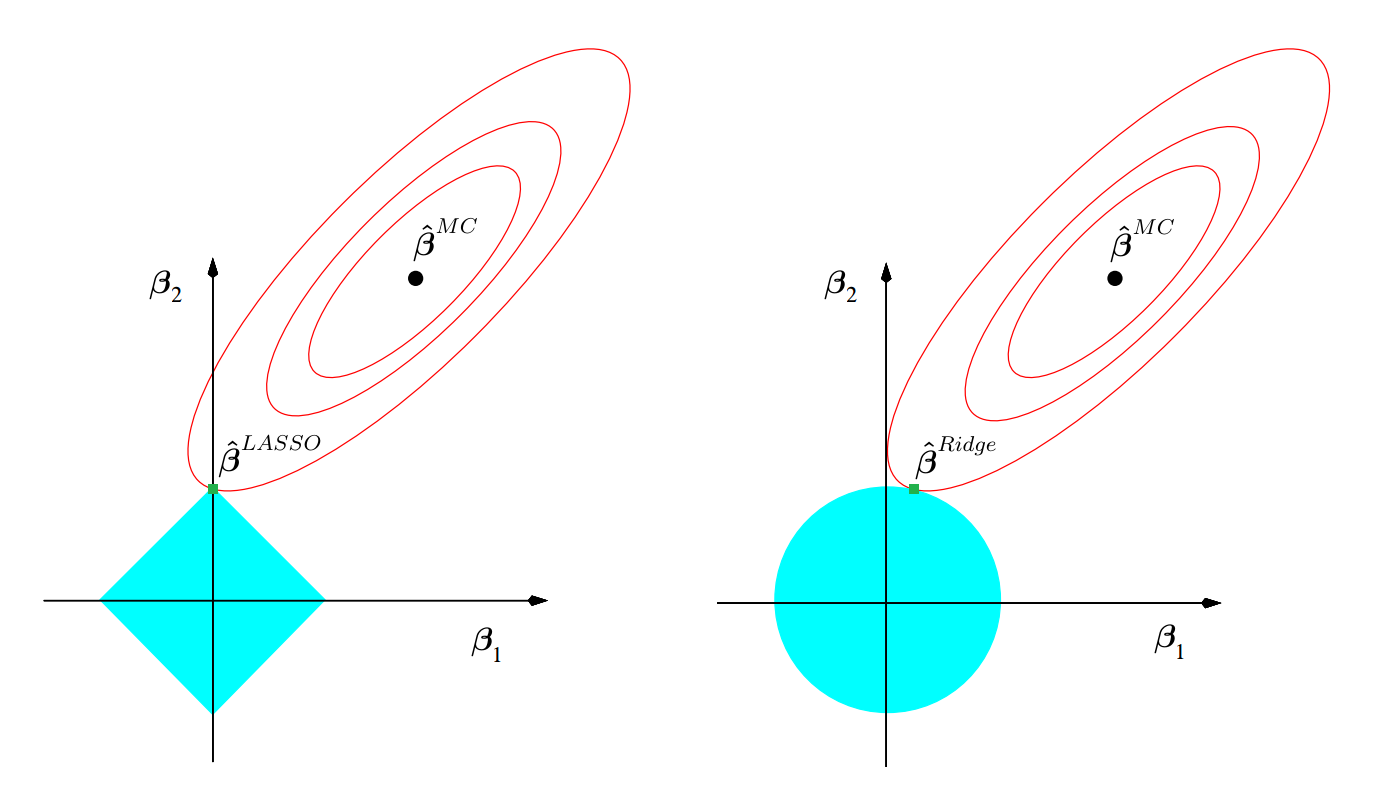
\includegraphics[height=3in]{2}
	\captionsetup{justification=justified}
	\caption{Representación geométrica de las condiciones para encontrar los estimadores LASSO (izquierda) y \textit{Ridge} (derecha) cuando $p=2$. Las áreas sólidas son las regiones de restricción ${|\beta_1|+|\beta_2| \leq t}$ (LASSO) y $\beta_1^2+\beta_2^2 \leq t$ (\textit{Ridge}), mientras que las elipses rojas son las curvas de nivel de la SCR. Figura adaptada de \textit{The Elements of Statistical Learning 2nd Edition} (p. 71), por Hastie, T., Tibshirani, R. y Friedman, J., 2009, New York, NY: Springer.}
	\label{fig: est_lasso_ridge_noorto}
\end{figure}

\section{Optimización Convexa}
Los estimadores en las regresiones \textit{Ridge} y LASSO plantean problemas de optimización convexos (ver Anexo I), mientras que la selección del mejor subconjunto es un problema de optimización no convexo de los más complejos.

La propiedad de convexidad es muy útil ya que asegura que el movimiento continuo que produce iterativamente un algoritmo en direcciones que disminuyen la función objetivo alcanzará eventualmente el mínimo global.

Asumiendo $\lambda > 0$, el problema de optimización \textit{Ridge} en (\ref{ridgePen}) es estrictamente convexo debido a la presencia de la penalidad $||\boldsymbol{\beta}||_2^2$. Esto es cierto para cualquier matriz de predictores $\boldsymbol{X}$, por lo que la solución \textit{Ridge} siempre está bien definida y, de hecho, está dada en forma cerrada por $\boldsymbol{\hat{\beta}}^{Ridge}=(\boldsymbol{X}^T\boldsymbol{X}+2\lambda \boldsymbol{I})^{-1}\boldsymbol{X}^T\boldsymbol{y}$.

Por el contrario, debido a la presencia de la penalidad $||\boldsymbol{\beta}||_1$, el problema LASSO en (\ref{lassoPen}) no siempre es estrictamente convexo y por lo tanto, no necesariamente tiene solución única. Es posible definir un problema modificado que siempre es estrictamente convexo, a través de la \textit{red elástica} \citep{zou2005regularization}:
\begin{equation}
\label{ElasticNet}
\operatornamewithlimits{min}\limits_{\boldsymbol{\beta} \in \mathbb{R}^p} \frac{1}{2}||\boldsymbol{y}-\boldsymbol{X}\boldsymbol{\beta}||_2^2+\lambda ||\boldsymbol{\beta}||_1+\delta ||\boldsymbol{\beta}||_2^2,
\end{equation}
donde ahora ambos $\lambda$, $\delta > 0$ son parámetros de suavizado. Además de garantizar unicidad para cualquier matriz $\boldsymbol{X}$, la \textit{red elástica} combina algunas de las propiedades predictivas deseables de la regresión \textit{Ridge} con las propiedades de dispersión de la regresión LASSO.

\section{Camino de Soluciones LASSO}
Usando las condiciones KKT (\ref{KKT}) y (\ref{Subgradiente}), es posible calcular la solución LASSO como función de $\lambda$, para todos los valores del parámetro de suavizado $\lambda \in [0,\infty)$. El conjunto de estimadores $\boldsymbol{\hat{\beta}}^{LASSO}(\lambda)$ recibe el nombre de camino de regularización o camino de soluciones del problema (\ref{lassoPen}). En otras palabras, el camino de regularización $\{\boldsymbol{\hat{\beta}}^{LASSO}(\lambda):\lambda\in [0,\infty)\}$ describe las soluciones LASSO a medida que varía el parámetro de suavizado $\lambda$.

Este camino de soluciones es una función continua lineal por tramos en $\lambda$. La continuidad del camino de soluciones permite que sólo sea necesario calcular y almacenar ciertos nodos ($\lambda_1 \geq \lambda_2 \geq ... \geq \lambda_r \geq 0$) y la solución LASSO en los mismos, a partir de los cuales por interpolación lineal pueden calcularse las soluciones para cualquier $\lambda \geq 0$.

Los nodos $\lambda_1 \geq \lambda_2 \geq ... \geq \lambda_r$ del camino de soluciones corresponden a valores de $\lambda$ en los que el conjunto activo $A(\lambda)=sop\left(\boldsymbol{\hat{\beta}}^{LASSO}(\lambda)\right)$ cambia. A medida que $\lambda$ disminuye desde $\infty$ a $0$, los nodos usualmente corresponderán a puntos en los que una variable ingresa al conjunto activo. Sin embargo, a medida que $\lambda$ disminuye, un nodo del camino LASSO puede también corresponder a un punto en el cual una variable abandona el conjunto activo, siendo este el motivo por el cual la regresión LASSO no produce modelos anidados y el número de nodos $r$ puede ser mucho mayor que $p$. En la Figura \ref{fig: LassoPath} se presenta un ejemplo del camino LASSO. Cada línea coloreada representa una componente de la solución LASSO $\hat{\beta}_j^{LASSO}(\lambda)$, $j=1, ..., p$ como función de $\lambda$. Las líneas de puntos verticales de color gris marcan los nodos $\lambda_1 \geq \lambda_2 \geq ... \geq \lambda_{11}$.

\begin{figure}[H]
	\centering
	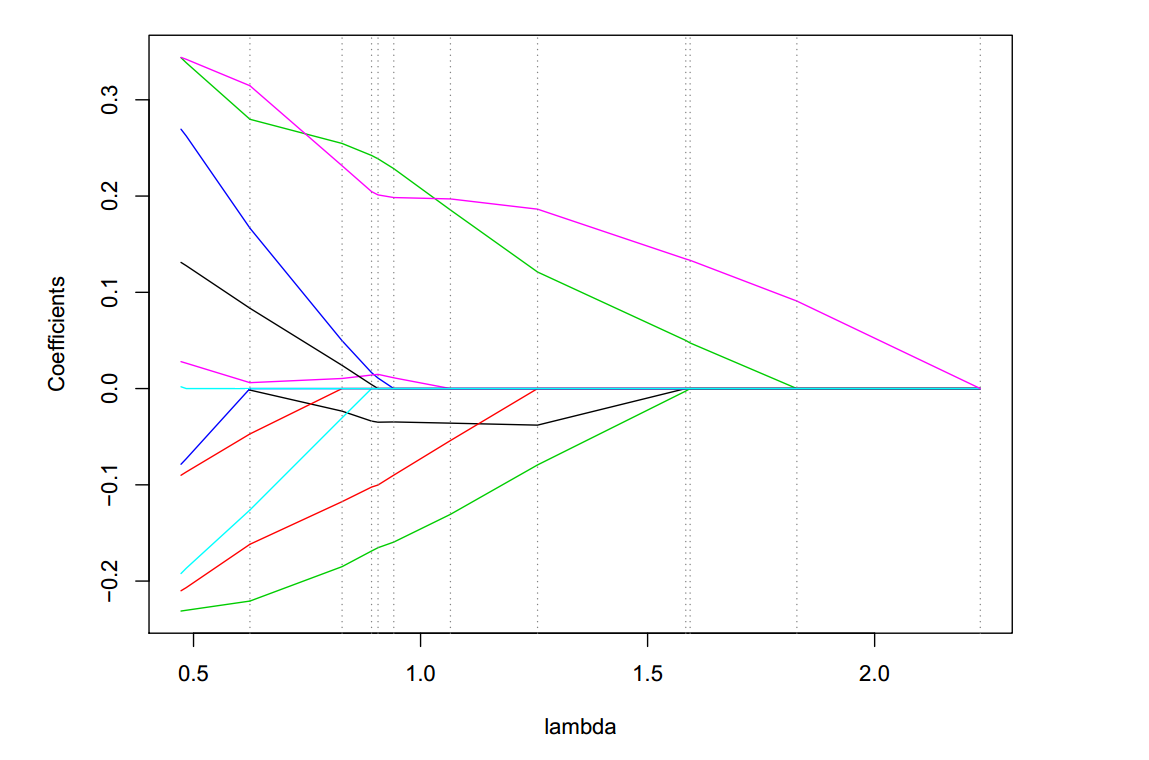
\includegraphics[height=3.75in]{6}
	\caption{Ejemplo de un camino de soluciones LASSO con 11 nodos}
	\label{fig: LassoPath}
	\end{figure}
	
El camino de soluciones LASSO fue descripto por \citet{osborne2000new} y \citet{efron2004least} y se construye a partir de la verificación iterativa de las condiciones KKT. 

Inicialmente se considera que $\lambda$ decrece desde $\infty$ y se define $\boldsymbol{\hat{\beta}}^{LASSO}(\lambda)=\boldsymbol{0}$. Para que efectivamente esta sea una solución LASSO válida, debe verificar la condición (\ref{KKT}), es decir, debe existir algún subgradiente $\boldsymbol{s}$ válido para esa solución. Luego de reemplazar $\boldsymbol{\hat{\beta}}^{LASSO}(\lambda)=\boldsymbol{0}$ en (\ref{KKT}), resulta $\boldsymbol{X}^T\boldsymbol{y}=\lambda \boldsymbol{s}$, donde $\boldsymbol{s}$ es un subgradiente de la norma $\ell_1$ evaluada en $\boldsymbol{\hat{\beta}}^{LASSO}(\lambda)=\boldsymbol{0}$, es decir, $s_j \in [-1,1]$ para todo $j=1, ...,p$. Para valores de $\lambda$ lo suficientemente grandes, esta implicación es cierta, ya que se puede elegir $\boldsymbol{s}=\boldsymbol{X}^T\boldsymbol{y}/\lambda$. Sin embargo, cuando $\lambda$ disminuye habiendo pasado el punto en el que $\lambda=|\boldsymbol{X}_j^T\boldsymbol{y}|$ para algún $j=1, ...,p$, $\boldsymbol{s}$ deja de ser un subgradiente válido para ese $j$, ya que $s_j > 1$ para $\hat{\beta}_j^{LASSO}=0$, lo cual no verifica las condiciones KKT. Resumiendo, $\boldsymbol{\hat{\beta}}^{LASSO}(\lambda)=\boldsymbol{0}$ es la solución LASSO para todo $\lambda\geq \lambda_1$, donde 
\begin{equation}
\label{Lambda1}
\lambda_1=\operatornamewithlimits{max}\limits_{j=1, ...,p} |\boldsymbol{X}_j^T\boldsymbol{y}|.
\end{equation}

Una vez alcanzado el primer nodo $\lambda_1$, cuando $\lambda$ decrece desde ese valor resulta necesario modificar $\boldsymbol{\hat{\beta}}^{LASSO}(\lambda)$ para que las condiciones KKT permanezcan satisfechas. Sea $j_1$ el índice de la variable que alcanza el máximo en (\ref{Lambda1}). Dado que el subgradiente tiene $|s_{j_1}|=1$ en $\lambda=\lambda_1$, se tiene ``permitido'' hacer que $\hat{\beta}_{j_1}$ sea distinto de cero. Entonces, a medida que $\lambda$ decrece desde $\lambda_1$, se considera fijar
\begin{equation}
\label{BJ1}
\begin{aligned}
\hat{\beta}_{j_1}^{LASSO}(\lambda)&=(\boldsymbol{X}_{j_1}^T\boldsymbol{X}_{j_1})^{-1}(\boldsymbol{X}_{j_1}^T\boldsymbol{y}-\lambda s_{j_1}), \\ \hat{\beta}_j^{LASSO}(\lambda)&=0,\text{ para todo } j\neq j_1,
\end{aligned}
\end{equation}
donde $s_{j_1}=sign(\boldsymbol{X}_{j_1}^T\boldsymbol{y})$. Esta consideración hace que $\boldsymbol{\hat{\beta}}^{LASSO}(\lambda)$ sea una función lineal por tramos continua en $\lambda$. El conjunto activo $A$ en este momento resulta $A=\{j_1\}$, mientras que $\boldsymbol{s}_A$, el conjunto que contiene los signos de los coeficientes estimados de las variables en $A$, también denominado conjunto de signos activos, resulta $\boldsymbol{s}_A=(s_{j_1})$.

Debido a que $\boldsymbol{X}\boldsymbol{\hat{\beta}}^{LASSO}=\boldsymbol{X}_{j_1}\hat{\beta}_{j_1}^{LASSO}$ por ser $\hat{\beta}_j^{LASSO}=0$ para todo $j \neq j_1$, las condiciones KKT para la variable $j_1$ son 
\begin{equation}
\boldsymbol{X}_{j_1}^T\left(\boldsymbol{y}-\boldsymbol{X}_{j_1}(\boldsymbol{X}_{j_1}^T\boldsymbol{X}_{j_1})^{-1}(\boldsymbol{X}_{j_1}\boldsymbol{y}-\lambda s_{j_1})\right)=\lambda s_{j_1},
\end{equation}
y para todo $j \neq j_1$
\begin{equation}
\label{Ineq1}
|\boldsymbol{X}_{j}^T\left(\boldsymbol{y}-\boldsymbol{X}_{j_1}(\boldsymbol{X}_{j_1}^T\boldsymbol{X}_{j_1})^{-1}(\boldsymbol{X}_{j_1}\boldsymbol{y}-\lambda s_{j_1})\right)| \leq \lambda.
\end{equation}
En (\ref{Ineq1}) se mantiene una desigualdad estricta cuando $\lambda=\lambda_1$ para todo $j \neq j_1$ y, por la continuidad de la solución $\boldsymbol{\hat{\beta}}^{LASSO}(\lambda)$ construida, esto se mantendrá cierto hasta que uno de los tramos lineales $\boldsymbol{X}_j^T(\boldsymbol{y}-\boldsymbol{X}_{j_1}(\boldsymbol{X}_{j_1}^T\boldsymbol{X}_{j_1})^{-1}(\boldsymbol{X}_{j_1}^T\boldsymbol{y}-\lambda s_{j_1}))$, con $j\neq j_1$, resulte igual a $\pm \lambda$, punto en el cual se deberá modificar nuevamente la solución, ya que de otro modo el gradiente implícito $s_j=\dfrac{\boldsymbol{X}_j^T(\boldsymbol{y}-\boldsymbol{X}_{j_1}(\boldsymbol{X}_{j_1}^T\boldsymbol{X}_{j_1})^{-1}(\boldsymbol{X}_{j_1}^T\boldsymbol{y}-\lambda s_{j_1}))}{\lambda}$ dejará de pertenecer al intervalo $[-1,1]$.

La linealidad del camino de soluciones permite calcular explícitamente el momento en el que uno de los tramos lineales se resulta igual a $\pm\lambda$, el cual recibe el nombre de \textit{hitting time}. A la variable que produce esta igualdad se la denominará variable \textit{hitting}.

La solución LASSO se mantiene igual a (\ref{BJ1}) para todo $\lambda_1 \geq \lambda \geq \lambda_2$, donde
\begin{equation}
\label{MaxLamb2}
\lambda_2=\operatornamewithlimits{max^+}\limits_{j\neq j_1, s_j \in \{-1,1\}} \frac{\boldsymbol{X}_j^T(\boldsymbol{I}-\boldsymbol{X}_{j_1}(\boldsymbol{X}_{j_1}^T\boldsymbol{X}_{j_1})^{-1}\boldsymbol{X}_{j_1})\boldsymbol{y}}{s_j-\boldsymbol{X}_j^T\boldsymbol{X}_{j_1}(\boldsymbol{X}_{j_1}^T\boldsymbol{X}_{j_1})^{-1}s_{j_1}},
\end{equation}
siendo max$^+$ el máximo sobre todos los argumentos que son menores que $\lambda_1$.

Ahora bien, sean $A=\{j_1,j_2\}$ y $\boldsymbol{s}_A=(s_{j_1},s_{j_2})$, donde $j_2$ y $s_2$ son la variable y el signo que alcanzan el máximo en (\ref{MaxLamb2}). A medida que $\lambda$ decrece desde $\lambda_2$, se considera fijar
\begin{equation}
\label{BAkkt}
\begin{aligned}
\boldsymbol{\hat{\beta}}_A^{LASSO}(\lambda)&=(\boldsymbol{X}_A^T\boldsymbol{X}_A)^{-1}(\boldsymbol{X}_A^T\boldsymbol{y}-\lambda \boldsymbol{s}_A), \\ \boldsymbol{\hat{\beta}}_{-A}^{LASSO}(\lambda)&=\boldsymbol{0},
\end{aligned}
\end{equation}
donde $\boldsymbol{\hat{\beta}}_A^{LASSO}$ se refiere a los coeficientes estimados de las variables del conjunto activo, mientras que $\boldsymbol{\hat{\beta}}_{-A}^{LASSO}$ se refiere a los de las variables que no forman parte de dicho conjunto.

Nuevamente, las condiciones KKT se verificarán para un conjunto de valores de $\lambda$, pero cuando uno de los $\boldsymbol{X}_j^T(\boldsymbol{y}-\boldsymbol{X}_A(\boldsymbol{X}_A^T\boldsymbol{X}_A)^{-1}(\boldsymbol{X}_A^T\boldsymbol{y}-\lambda \boldsymbol{s}_A)), \hspace{0.2cm} j \notin A$, resulte igual a $\pm \lambda$, se deberá volver a modificar el estimador $\boldsymbol{\hat{\beta}}^{LASSO}$ para que se satisfagan dichas condiciones.

Al disminuir $\lambda$ cuando el conjunto activo está formado por dos o más variables, además de tener en cuenta el siguiente \textit{hitting time}, es necesario verificar que ninguna de las componentes activas de la solución calculada en (\ref{BAkkt}) cruce el valor cero, porque pasado ese punto, $\boldsymbol{s}_A$ dejará de ser un subgradiente válido para esas componentes activas. A modo de ejemplo, si $\hat{\beta}_{j}^{LASSO}$ pasa de positivo a negativo, $s_j=1$ dejará de ser un subgradiente válido para ese $j$.

El momento en el que una componente $\hat{\beta}_j^{LASSO}$ cambia de signo recibe el nombre de \textit{crossing time}, y también puede ser calculado explícitamente debido a la linealidad del camino de soluciones. A la variable cuya componente cambia de signo se la denominará variable \textit{crossing}. 

Por lo tanto, se sostiene que (\ref{BAkkt}) es la solución LASSO para todo $\lambda_2 \geq \lambda \geq \lambda_3$, donde $\lambda_3$ es el máximo entre el siguiente \textit{hitting time} y \textit{crossing time}. Si $\lambda_3$ corresponde a un \textit{hitting time}, la variable \textit{hitting} se agrega al conjunto activo. Por el contrario, si corresponde a un \textit{crossing time}, se remueve la variable \textit{crossing} de dicho conjunto. Cualquiera sea el caso, es necesario volver a calcular la solución LASSO usando (\ref{BAkkt}) de modo que se verifiquen las condiciones KKT. Luego, se calculan los siguientes \textit{hitting} y \textit{crossing times}, se verifica si es necesario agregar o eliminar una variable al conjunto activo y vuelve a calcularse la solución LASSO. Este procedimiento se repite mientras $\lambda > 0$. El algoritmo del camino LASSO se resume a continuación:

{\setstretch{1.0}
\subsection*{Algoritmo 1. Algoritmo del Camino de Soluciones LASSO}
Dados $\boldsymbol{X}$ e $\boldsymbol{y}$
\begin{itemize}
\item Comenzar con el contador de iteración $k=0$, parámetro de regularización $\lambda_0=\infty$, conjunto activo $A=\emptyset$ y signos activos $\boldsymbol{s}_A=\emptyset$.
\item Mientras $\lambda_k > 0$:
\begin{enumerate}
\item Calcular la solución LASSO a medida que $\lambda$ decrece desde $\lambda_k$ a través de
\begin{equation*}
\begin{aligned}
\boldsymbol{\hat{\beta}}_A(\lambda)&=(\boldsymbol{X}_A^T\boldsymbol{X}_A)^{-1}(\boldsymbol{X}_A^T\boldsymbol{y}-\lambda \boldsymbol{s}_A), \\ \boldsymbol{\hat{\beta}}_{-A}(\lambda)&=\boldsymbol{0},
\end{aligned}
\end{equation*}
\item Calcular el siguiente \textit{hitting time}
\begin{equation*}
\lambda_{k+1}^{hit}=\operatornamewithlimits{max^+}\limits_{j\neq A, s_j \in \{-1,1\}} \frac{\boldsymbol{X}_j^T(\boldsymbol{I}-\boldsymbol{X}_A(\boldsymbol{X}_A^T\boldsymbol{X}_A)^{-1}\boldsymbol{X}_A)\boldsymbol{y}}{s_j-\boldsymbol{X}_j^T\boldsymbol{X}_A(\boldsymbol{X}_A^T\boldsymbol{X}_A)^{-1}\boldsymbol{s}_A},
\end{equation*}
donde max$^+$ denota el máximo de los argumentos menores que $\lambda_k$.
\item Calcular el siguiente \textit{crossing time}
\begin{equation*}
\lambda_{k+1}^{cross}=\operatornamewithlimits{max^+}\limits_{j \in A} \frac{[(\boldsymbol{X}_A^T\boldsymbol{X}_A)^{-1}\boldsymbol{X}_A)\boldsymbol{y}]_j}{[(\boldsymbol{X}_A^T\boldsymbol{X}_A)^{-1}\boldsymbol{s}_A]_j},
\end{equation*}
\item Decrecer $\lambda$ hasta $\lambda_{k+1}$, definido por
\begin{equation*}
\lambda_{k+1}=\text{max}\{\lambda_{k+1}^{hit},\lambda_{k+1}^{cross}\}
\end{equation*}
\item Si $\lambda_{k+1}^{hit} > \lambda_{k+1}^{cross}$ agregar la variable \textit{hitting} al conjunto $A$ y su signo a $\boldsymbol{s}_A$; caso contrario, remover la variable \textit{crossing} de $A$ y su signo de $\boldsymbol{s}_A$. Actualizar $k=k+1$. 
\end{enumerate}
\end{itemize}
}

\vspace{0.8cm}

El algoritmo del camino de soluciones LASSO presentado en el Algoritmo 1 también es llamado Regresión del Menor Ángulo en modo LASSO debido a su estrecha relación con otro algoritmo conocido como Regresión del Menor Ángulo o LARS (\textit{Least Angle Regression}), el cual fue presentado por \citet{efron2004least} y también es utilizado para el ajuste de modelos lineales en grandes dimensiones. La única diferencia radica en que LARS no evita que las componentes de las soluciones crucen el cero.

Otro algoritmo que puede ser utilizado como alternativa para el cálculo del camino de soluciones LASSO es el denominado \textit{Coordinate Descent} \citep{friedman2007pathwise} \citep{friedman2010regularization}. Este algoritmo mantiene fijo el parámetro de penalidad $\lambda$ en (\ref{BETA_LASSO}) y optimiza sucesivamente sobre cada parámetro $\beta_j$ $j=1,...,p$ hasta lograr la convergencia del proceso. Esto se repite para distintos valores de $\lambda$, obteniendo el camino de soluciones LASSO. \textit{Coordinate Descent} es más rápido que LARS, especialmente en problemas de gran magnitud. Además, puede proporcionar soluciones para un conjunto determinado de valores de $\lambda$, a diferencia de LARS que necesariamente calcula todo el camino de soluciones.

Este algoritmo se encuentra disponible en forma gratuita en el paquete \textbf{glmnet} de MATLAB o R \citep{friedman2009glmnet} y es el que ha sido utilizado en esta tesina. En el Anexo II se describe el uso del paquete en R, con algunas instrucciones y particularidades del mismo. 

En el Anexo III se presentan programas disponibles para la obtención de los estimadores de los métodos estudiados.

\chapter{Resultados}
En este capítulo se presentan los resultados de un estudio por simulación para comparar las propiedades de los estimadores \textit{Ridge} y LASSO en diferentes escenarios. Los estimadores mínimo-cuadráticos son incluidos en la comparación sólo en los casos donde existen estimaciones únicas.

Dado que los métodos \textit{Ridge} y LASSO mejoran las estimaciones obtenidas en presencia de muchos parámetros no significativos en un modelo de regresión lineal, los escenarios previstos consideran la situación extrema de existencia de parámetros nulos, para identificar si el método de estimación los reconoce como tal.

La eficiencia de los modelos se evalúa a través del Error Cuadrático Medio (ECM) y las propiedades de los estimadores a través de su distribución empírica.

Para las simulaciones se utiliza el paquete \textbf{simulator} del software R. Este es un paquete que agiliza el proceso de realizar simulaciones al crear una infraestructura común que puede usarse y reutilizarse fácilmente \citep{bien2016simulator}. El \textbf{simulator} divide la simulación en cuatro componentes:
\begin{enumerate}
\item \textbf{Modelo}: el modelo estadístico que determina cómo se generan los datos.
\item \textbf{Métodos}: los procedimientos estadísticos que se desean comparar. Dados los datos, cada método produce una salida en forma de estimador, predicción o decisión.
\item \textbf{Métricas}: medidas que evalúan el desempeño de los métodos utilizando las salidas obtenidas a partir de los datos.
\item \textbf{Gráficos}: representación gráfica de las métricas evaluadas para los distintos métodos bajo los distintos escenarios simulados.
\end{enumerate}
El paquete utiliza el código de las primeras tres componentes para realizar la simulación, mientras que la cuarta componente permite presentar los resultados del estudio. En particular, siguiendo el ejemplo ``\textit{Betting on sparsity with the LASSO}'' \citep{bien2016simulator}, en este trabajo se adoptó un modelo lineal esparcido y se calcularon los estimadores LASSO (a través del paquete \textbf{glmnet}) y los estimadores \textit{Ridge} (a través de la codificación de (\ref{Ridge_estimator_DVS})). Los estimadores MC también se obtuvieron utilizando el paquete \textbf{glmnet}.

En la Sección 4.1 se explicita el diseño del estudio por simulación. En la Sección 4.2 se compara la capacidad predictiva de los estimadores. En las Secciones 4.3 y 4.4 se estudian las propiedades distribucionales de los estimadores de parámetros no nulos y nulos respectivamente. Finalmente, en la Sección 4.5 se estudia la capacidad del método LASSO de obtener estimaciones nulas, tanto cuando $\beta=0$ (situación deseable) como cuando $\beta=1$ (situación no deseable).

\section{Diseño del Estudio por Simulación}
Se plantearon tres situaciones variando el número de variables explicativas en función del tamaño de muestra, el cual fue fijado en $n = 100$. Las variantes elegidas para el número de predictores fueron $p = n = 100$ (Situación 1), $p = 2n = 200$ (Situación 2) y $p = 4n = 400$ (Situación 3). Para cada combinación de $n$ y $p$ se consideraron modelos lineales múltiples esparcidos, es decir, modelos con gran cantidad de parámetros iguales a cero, a partir de los cuales se simularon valores de una variable respuesta $y$. El modelo supuesto es:
\begin{equation}
\boldsymbol{y} = \boldsymbol{X}\boldsymbol{\beta}_{npk} + \phi \boldsymbol{\epsilon},
\end{equation} 
siendo,

\begin{itemize}
\item $\boldsymbol{y}$ el vector de respuestas de dimensión $100 \times 1$

\item $\boldsymbol{X}$ una matriz de predictores de dimensión $100 \times p$ cuyos elementos fueron simulados de una distribución $N(0,1)$

\item $\boldsymbol{\beta}_{npk} = \boldsymbol{\beta}_\gamma$ un vector de parámetros de dimensión $p \times 1$, a cuyas $k$ primeras componentes se les asignó un valor igual a uno, y a las $p - k$ restantes el valor cero. El valor de $k$ refleja el grado de esparcimiento del modelo

\item $\boldsymbol{\epsilon}$ un vector de errores aleatorios de dimensión $100 \times 1$ cuyas componentes fueron simuladas de una distribución $N(0,1)$

\item $\phi$ un parámetro de variabilidad que se supuso $\phi = \sqrt{\dfrac{\sum_{i=1}^{100} \left(\boldsymbol{X}\boldsymbol{\beta}_{npk}\right)_i^2}{snr \times 100}}$, tomando el \textit{signal-to-noise-ratio} ($snr$) igual a 2. La elección de este parámetro de variabilidad permite conseguir variantes asociadas al grado de esparcimiento \citep{bien2016simulator}
\end{itemize}

La matriz de predictores $\boldsymbol{X}$ utilizada en la simulación de valores de la respuesta $\boldsymbol{y}$ se mantuvo invariante para los distintos modelos dentro de cada una de las tres situaciones.

Se consideran variantes para $k$ desde 2 hasta $\dfrac{p}{2}$, donde a medida que $k$ aumenta, se tiene un mayor número de parámetros distintos de cero, lo que disminuye el grado de esparcimiento del modelo.

En la Situación 1 se construyeron un total de 13 modelos, eligiendo los siguientes valores no equidistantes de $k$: 2, 4, 6, 8, 10, 15, 20, 25, 30, 35, 40, 45 y 50.

En la Situación 2 se construyeron un total de 18 modelos, tomando como valores de $k$ a las 13 variantes de la Situación 1 y agregando los valores 60, 70, 80, 90 y 100.

En la Situación 3, se construyeron un total de 11 modelos, eligiendo los siguientes valores para $k$: 2, 5, 10, 20, 30, 40, 50, 75, 100, 150 y 200.

Cada combinación de $n$, $p$ y $k$ se considera como un escenario donde se compara la eficiencia de los métodos ($\gamma=1,...,42$).

En cada uno de los 42 escenarios definidos se realizaron 1.000 simulaciones de $\boldsymbol{y}$ con los que se obtuvieron los estimadores de $\boldsymbol{\beta}$ correspondientes a las regresiones \textit{Ridge} y LASSO para 50 valores diferentes del parámetro de suavizado $\lambda$, reteniendo en cada método aquella solución $\boldsymbol{\hat{\beta}}_\lambda$ que produjera el menor ECM. 

En los 13 escenarios de la Situación 1, donde el número de observaciones es igual al número de variables explicativas, también se obtuvo el estimador mínimo-cuadrático. En los otros casos no existe solución única al problema de optimización mínimo-cuadrático, por lo cual no tiene sentido incluirlos en la comparación.

\subsection{Criterios de Comparación entre Modelos}
Para comparar los modelos se tuvieron en cuenta dos criterios: la capacidad predictiva y las propiedades de los estimadores. Para el estudio de las propiedades de los estimadores se construyeron las distribuciones empíricas agrupando aquéllos que estiman parámetros $\beta=0$ ($\hat{\beta}^{(0)}$) y los que estiman parámetros $\beta=1$ ($\hat{\beta}^{(1)}$).

Dado que los estimadores LASSO son conocidos por su capacidad de estimar como nulos a una gran cantidad de los parámetros del modelo, lo cual es deseable en el contexto de grandes dimensiones donde el número de variables explicativas puede ser excesivo, se enfoca como medida de eficiencia a las probabilidades que estos estimadores nulos estén reconociendo efectivamente o no a un parámetro sin efecto. En particular, se proponen dos medidas específicas que reflejan la capacidad del método LASSO de obtener estimaciones nulas, tanto para el caso $\beta = 1$ (situación no deseable) como $\beta = 0$ (situación deseable).

Las medidas consideradas en las comparaciones son:
\begin{enumerate}
\item Promedio de Errores Cuadráticos Medios ($\overline{ECM}$)

Para cada combinación de $n$, $p$ y $k$ ($\gamma$), se calcula para cada método $q$, $q \in $ \{MC, \textit{Ridge}, LASSO\} o \{\textit{Ridge}, LASSO\} según el escenario, el promedio de los ECM entre las 1.000 simulaciones.
\begin{equation}
\overline{ECM}_{q\gamma}=\dfrac{1}{1000}\sum_{i=1}^{1000} ECM_{q\gamma i}=\dfrac{1}{1000}\sum_{i=1}^{1000} \dfrac{||\boldsymbol{\hat{\beta}}_{q\gamma i}-\boldsymbol{\beta}_{\gamma}||_2^2}{p}
\end{equation}
\item Promedio de los estimadores de parámetros $\beta = 1$ y $\beta = 0$

Para cada método $q \in $ \{MC, \textit{Ridge}, LASSO\} se define el promedio de los estimadores $\hat{\beta}^{(1)}$ como
\begin{equation}
\overline{\hat{\beta}}_{q\gamma}^{(1)}=\dfrac{1}{k \times 1000} \sum_{i=1}^{1000} \sum_{l=1}^k \hat{\beta}_{q\gamma li}
\end{equation}

mientras que el promedio de los estimadores $\hat{\beta}^{(0)}$ resulta
\begin{equation}
\overline{\hat{\beta}}_{q\gamma}^{(0)}=\dfrac{1}{(p-k) \times 1000} \sum_{i=1}^{1000} \sum_{l=k+1}^p \hat{\beta}_{q\gamma li}
\end{equation}
\item Variabilidad de las distribuciones muestrales de los estimadores de $\beta = 1$ y $\beta = 0$

Para cada método $q \in $ \{MC, \textit{Ridge}, LASSO\} se define el desvío estándar de los estimadores $\hat{\beta}^{(1)}$ como
\begin{equation}
S_{\hat{\beta}_{q\gamma}}^{(1)}=\sqrt{\dfrac{1}{k \times 1000-1} \sum_{i=1}^{1000} \sum_{l=1}^k \left(\hat{\beta}_{q\gamma li}-\overline{\hat{\beta}}_{q\gamma}^{(1)}\right)^2},
\end{equation}
mientras que el desvío estándar de los estimadores de parámetros $\beta = 0$ resulta
\begin{equation}
S_{\hat{\beta}_{q\gamma}}^{(0)}=\sqrt{\dfrac{1}{(p-k) \times 1000-1} \sum_{i=1}^{1000} \sum_{l=k+1}^p \left(\hat{\beta}_{q\gamma li}-\overline{\hat{\beta}}_{q\gamma}^{(0)}\right)^2}
\end{equation}
\item Porcentaje de parámetros nulos estimados por cero por el método LASSO

Esta medida se calcula multiplicando por 100 al cociente entre el número de estimadores de $\beta=0$ que son 0 y el número de parámetros $\beta=0$. En símbolos:
\begin{equation}
\label{eq: ptj 0 bien}
\left(\dfrac{1}{(p-k) \times 1000}\sum_{i=1}^{1000}\sum_{l=k+1}^p I(\hat{\beta}_{q\gamma li} = 0)\right)\times 100,
\end{equation}
donde $q = LASSO$. La expresión \ref{eq: ptj 0 bien} se puede asimilar al concepto de una sensibilidad de los estimadores LASSO para detectar los parámetros no significativos del modelo.

\item Porcentaje de parámetros no nulos estimados por cero por el método LASSO 

Esta medida se calcula multiplicando por 100 al cociente entre el número de estimadores de $\beta=1$ que son 0 y el número de parámetros $\beta=1$. En símbolos:
\begin{equation}
\label{eq: ptj 1 mal}
\left(\dfrac{1}{k \times 1000}\sum_{i=1}^{1000}\sum_{l=1}^k I(\hat{\beta}_{q\gamma li} = 0)\right)\times 100,
\end{equation}
donde $q=LASSO$. La expresión \ref{eq: ptj 1 mal} puede asimilarse a una probabilidad de error de la regresión LASSO en el sentido de un falso positivo.
\end{enumerate}

\newpage

{\setstretch{1.5}
\section[Capacidad Predictiva de los Estimadores. Comparación del $\overline{ECM}$]{Capacidad Predictiva de los Estimadores. \\ Comparación del $\overline{ECM}$.}
}

En esta Sección se evalúa, para cada combinación de $n$ y $p$, cómo se comportan los $\overline{ECM}$ de cada método a medida que varía el grado de esparcimiento ($k$).

\subsection*{Situación 1 ($p=n=100$)}

\begin{figure}[H]
	\centering
	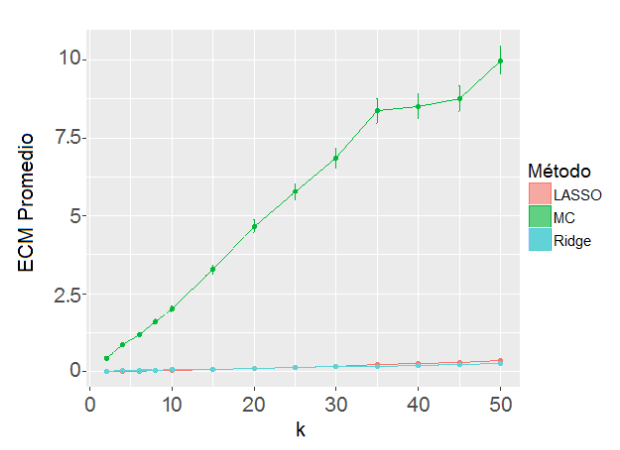
\includegraphics[height=3in]{ECM P 100 MC}
	\caption{$\overline{ECM}$ de los métodos MC, \textit{Ridge} y LASSO \\ para variantes de $k$. Caso $p=n=100$}
	\label{fig: ECM P100 MC}
\end{figure}

El $\overline{ECM}$ de los estimadores mínimo-cuadráticos aumenta en forma severa a medida que $k$ crece, mientras que el de los métodos de regularización presenta la misma tendencia pero con un crecimiento mucho más lento (Figura \ref{fig: ECM P100 MC}). Esta figura, debido a las dimensiones de las escalas, no muestra diferencias entre los $\overline{ECM}$ de los estimadores \textit{Ridge} y LASSO, sin embargo, no son iguales. Para poder comparar estos dos métodos, se presenta la Figura \ref{fig: ECM P100} que no considera al método de mínimos cuadrados y se concentra en los valores más pequeños del eje de las ordenadas, evidenciándose las diferencias en el comportamiento de los métodos de regularización.

\begin{figure}[H]
	\centering
	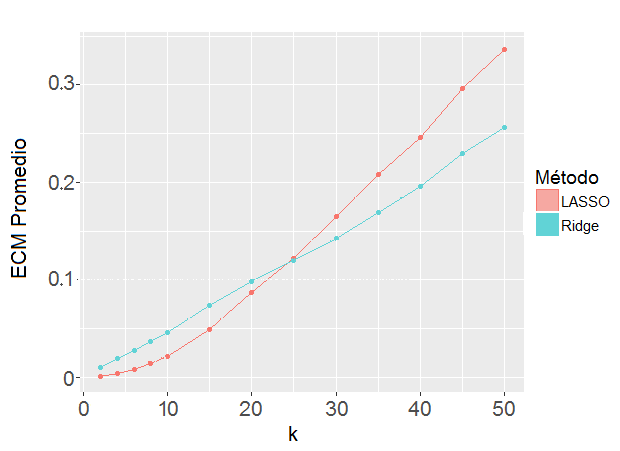
\includegraphics[height=3in]{ECM P 100}
	\caption{$\overline{ECM}$ de los métodos \textit{Ridge} y LASSO \\ para variantes de $k$. Caso $p=n=100$}
	\label{fig: ECM P100}
\end{figure}

Para valores de $k$ pequeños, menores que $25$, el $\overline{ECM}$ de los estimadores LASSO es menor que el de los estimadores \textit{Ridge} (Figura \ref{fig: ECM P100}). Sin embargo, a medida que $k$ se acerca a 25, la diferencia entre los métodos disminuye. A partir de este valor, el $\overline{ECM}$ de los estimadores \textit{Ridge} es menor que el de los LASSO, y la diferencia entre ellos aumenta con $k$. De todos modos, con valores de $k$ grandes ambos métodos empeoran su desempeño con respecto a los resultados obtenidos para valores de $k$ pequeños.

\subsection*{Situación 2 ($p=2n=200$)}
En la Figura \ref{fig: ECM P200} se observa nuevamente que LASSO tiene un mejor desempeño que \textit{Ridge} en cuanto al $\overline{ECM}$ para modelos con mayor grado de esparcimiento, y que esta relación se revierte en problemas más densos. Del mismo modo, con valores de $k$ grandes ambos métodos empeoran su desempeño con respecto a los resultados obtenidos para valores de $k$ pequeños. En este caso, en $k=\dfrac{p}{2}$ se observan $\overline{ECM}$ mayores que los observados para esa misma proporción de $k$ en la Situación 1 (Figura \ref{fig: ECM P100}). 

\begin{figure}[H]
	\centering
	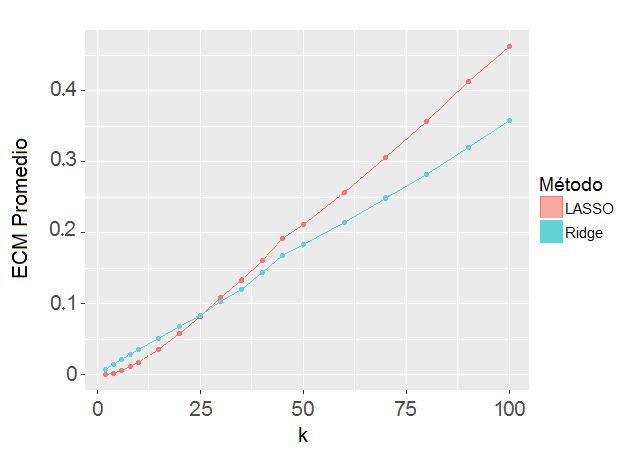
\includegraphics[height=3in]{ECM P 200}
	\caption{$\overline{ECM}$ de los métodos \textit{Ridge} y LASSO \\ para variantes de $k$. Caso $p=2n=200$}
	\label{fig: ECM P200}
\end{figure}

\subsection*{Situación 3 ($p=4n=400$)}

\begin{figure}[H]
	\centering
	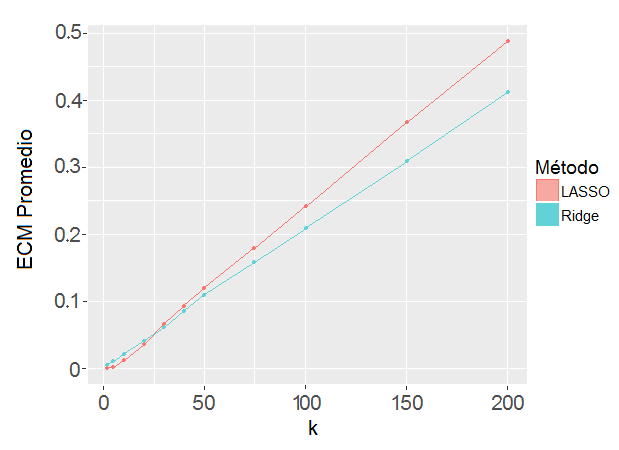
\includegraphics[height=3in]{ECM P 400}
	\caption{$\overline{ECM}$ de los métodos \textit{Ridge} y LASSO \\ para variantes de $k$. Caso $p=4n=400$}
	\label{fig: ECM P400}
\end{figure}

En la Situación 3, el comportamiento respecto de la capacidad predictiva de \textit{Ridge} y LASSO  (Figura \ref{fig: ECM P400}) repite lo observado en las Situaciones 1 y 2. Los $\overline{ECM}$ aumentan con $k$ y las curvas se cruzan nuevamente aproximadamente en el valor $k=25$.

{\setstretch{1.5}
\section{Propiedades Distribucionales de Estimadores $\hat{\beta}^{(1)}$}}
En esta Sección se comparan los promedios y coeficientes de variación de los estimadores de los parámetros $\beta=1$ para cada método en cada escenario, separando nuevamente los resultados por situación. El cálculo de los coeficientes de variación es necesario para comparar las variabilidades de las distribuciones frente a promedios diferentes. Además, para completar la descripción del comportamiento aleatorio de los estimadores, se muestran gráficamente sus distribuciones empíricas para cada método. Se han seleccionado sólo algunos escenarios debido a la regularidad de los resultados encontrados. Los casos restantes pueden consultarse en el Anexo IV.

\subsection*{Situación 1 ($p=n=100$)}
\begin{table}[H]
\centering
\caption{Medidas características de las distribuciones de los estimadores $\hat{\beta}^{(1)}$ para cada método y variantes de $k$. Caso $p=n=100$.}
\label{tab: sit 1 B 1 med std}
\footnotesize
\begin{tabular}{c|ccc|ccc|ccc}
 \multirow{3}{*}[-2em]{\textbf{k}} & \multicolumn{9}{c}{\textbf{Método}} \\[2ex]
 & \multicolumn{3}{c}{\textbf{MC}} & \multicolumn{3}{c}{\textbf{Ridge}} & \multicolumn{3}{c}{\textbf{LASSO}} \\[2ex]
 & \scriptsize\makecell{\textbf{Promedio} \\ $\overline{\hat{\beta}}_{MC \hspace{0.05cm} \gamma}^{(1)}$} & \scriptsize\makecell{\textbf{Desvío} \\ \textbf{Estándar} \\ $S_{\hat{\beta}_{MC \hspace{0.05cm} \gamma}}^{(1)}$} & \scriptsize\textbf{CV(\%)} & \scriptsize\makecell{\textbf{Promedio} \\ $\overline{\hat{\beta}}_{Ridge \hspace{0.05cm} \gamma}^{(1)}$} & \scriptsize\makecell{\textbf{Desvío} \\ \textbf{Estándar} \\ $S_{\hat{\beta}_{Ridge \hspace{0.05cm} \gamma}}^{(1)}$} & \scriptsize\textbf{CV(\%)} & \scriptsize\makecell{\textbf{Promedio} \\ $\overline{\hat{\beta}}_{LASSO \hspace{0.05cm} \gamma}^{(1)}$} & \scriptsize\makecell{\textbf{Desvío} \\ \textbf{Estándar} \\ $S_{\hat{\beta}_{LASSO \hspace{0.05cm} \gamma}}^{(1)}$} & \scriptsize\textbf{CV(\%)} \\ \hline
\textbf{2} & 0,9928 & 0,6744 & \hspace{0.05cm} 67,93 & 0,5122 & 0,0739 & 14,43 & 0,8197 & 0,0908 & \hspace{0.05cm} 11,08 \\
\textbf{4} & 1,0057 & 0,9940 & \hspace{0.05cm} 98,84 & 0,5160 & 0,1020 & 19,77 & 0,7704 & 0,1427 & \hspace{0.05cm} 18,52 \\
\textbf{6} & 1,0089 & 1,0369 & 102,78 & 0,5437 & 0,1229 & 22,60 & 0,7480 & 0,1711 & \hspace{0.05cm} 22,87 \\
\textbf{8} & 1,0043 & 1,1528 & 114,79 & 0,5430 & 0,1525 & 28,08 & 0,7209 & 0,2091 & \hspace{0.05cm} 29,01 \\
\textbf{10} & 0,9958 & 1,4126 & 141,86 & 0,5346 & 0,1595 & 29,84 & 0,7052 & 0,2371 & \hspace{0.05cm} 33,62 \\
\textbf{15} & 0,9828 & 1,7178 & 174,79 & 0,5007 & 0,1863 & 37,21 & 0,6515 & 0,3269 & \hspace{0.05cm} 50,18 \\
\textbf{20} & 0,9890 & 1,9890 & 201,11 & 0,4970 & 0,2184 & 43,94 & 0,6077 & 0,3978 & \hspace{0.05cm} 65,46 \\
\textbf{25} & 0,9981 & 2,2679 & 227,22 & 0,5241 & 0,2469 & 47,11 & 0,5969 & 0,4375 & \hspace{0.05cm} 73,30 \\
\textbf{30} & 0,9942 & 2,6416 & 265,70 & 0,5268 & 0,2701 & 51,27 & 0,5686 & 0,4775 & \hspace{0.05cm} 83,98 \\
\textbf{35} & 0,9922 & 2,8652 & 288,77 & 0,5171 & 0,2966 & 57,36 & 0,5381 & 0,5032 & \hspace{0.05cm} 93,51 \\
\textbf{40} & 0,9786 & 2,9323 & 299,64 & 0,5151 & 0,3192 & 61,97 & 0,5178 & 0,5111 & \hspace{0.05cm} 98,71 \\
\textbf{45} & 0,9792 & 3,0316 & 309,60 & 0,5022 & 0,3452 & 68,74 & 0,4925 & 0,5245 & 106,50 \\
\textbf{50} & 0,9804 & 3,2023 & 326,63 & 0,4965 & 0,3587 & 72,25 & 0,4707 & 0,5288 & 112,34
\end{tabular}
\end{table}

Respecto de la propiedad de insesgamiento, la Tabla \ref{tab: sit 1 B 1 med std} corrobora que los estimadores MC tienen promedios muy cercanos a 1, el verdadero valor del parámetro, mientras que los estimadores \textit{Ridge} son sesgados, con promedios cercanos a 0,50 para todo $k$. Los estimadores LASSO también son sesgados, pero el sesgo aumenta con $k$. Cuando $k$ es pequeño, los promedios de estos últimos son cercanos al valor 1 (alrededor de 0,75), siendo comparativamente mejores que los \textit{Ridge} en modelos con ese grado de esparcimiento.

La variabilidad de los estimadores MC es mucho mayor que la de los métodos de regularización para todo $k$. Al comparar los coeficientes de variación de los estimadores \textit{Ridge} y LASSO, se observa que los de LASSO son menores que los de \textit{Ridge} en los modelos más esparcidos y que esta relación se revierte a medida que aumenta $k$. Para todos los métodos, los coeficientes de variación aumentan con $k$.

En la Figura \ref{fig: P100 B1 MC} se comparan las distribuciones de los estimadores de $\beta=1$ para los tres métodos de estimación, evidenciando algunas características adicionales a las señaladas a partir del análisis de la Tabla \ref{tab: sit 1 B 1 med std}. Las distribuciones de los estimadores presentan un contorno totalmente distinto según el método aplicado. Las diferencias más notables se dan entre MC y los dos métodos de regularización. La distribución de los estimadores MC se asemeja a la distribución Normal y es mucho más dispersa. Para captar con mayor detalle las diferencias entre las regresiones \textit{Ridge} y LASSO, la Figura \ref{fig: P100 B1} repite las distribuciones de los estimadores $\hat{\beta}^{(1)}$ omitiendo los obtenidos por MC.

Los estimadores \textit{Ridge} muestran distribuciones empíricas con forma campanular para todo $k$, evidenciando su distribución teórica Normal, con menor dispersión para $k$ pequeños. A medida que $k$ crece, la distribución se achata y se expande su variabilidad (Figura \ref{fig: P100 B1}). Para valores de $k$ pequeños, los estimadores LASSO también muestran una distribución de frecuencias campanular, pero para $k \geq 20$ (aproximadamente) se encuentra un gran porcentaje de estimadores nulos aún cuando el parámetro a estimar es igual a 1. Esta característica es la que empeora el sesgo evidenciado en la Tabla \ref{tab: sit 1 B 1 med std}.

\begin{figure}[H]
\centering
\subfloat[$k = 2$]{
  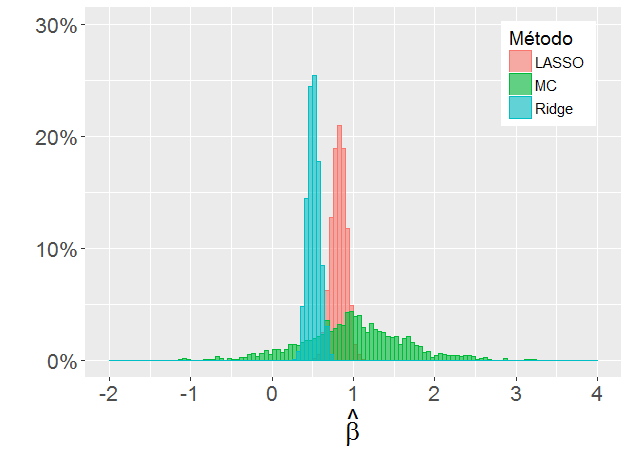
\includegraphics[width=7.95cm]{P 100 K 02 B1 MC}
}
\subfloat[$k = 10$]{
  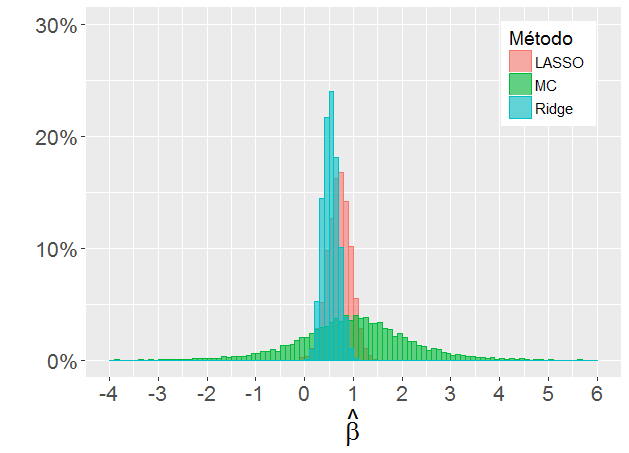
\includegraphics[width=7.95cm]{P 100 K 10 B1 MC}
}
\hspace{0mm}
\subfloat[$k = 20$]{
  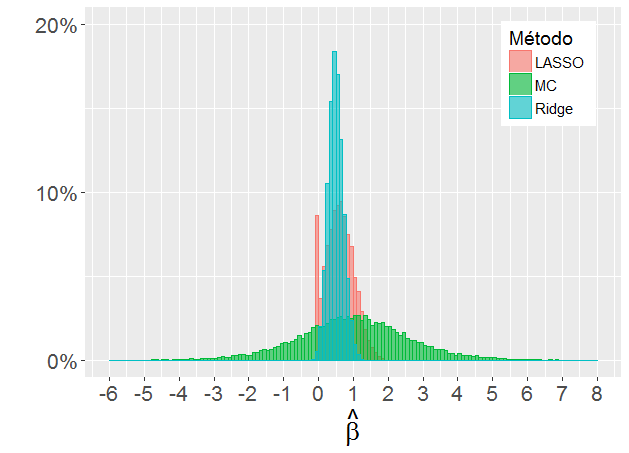
\includegraphics[width=7.95cm]{P 100 K 20 B1 MC}
}
\subfloat[$k = 30 $]{
  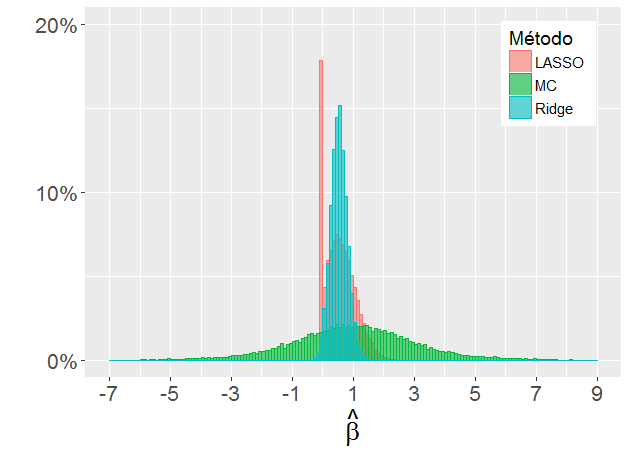
\includegraphics[width=7.95cm]{P 100 K 30 B1 MC}
}
\hspace{0mm}
\subfloat[$k = 40$]{
  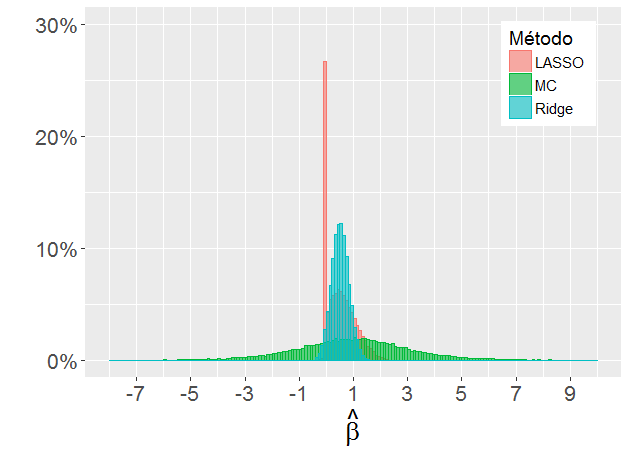
\includegraphics[width=7.95cm]{P 100 K 40 B1 MC}
}
\subfloat[$k = 50$]{
  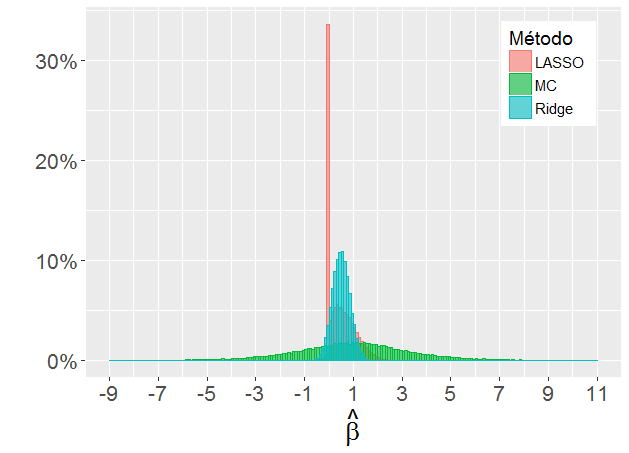
\includegraphics[width=7.95cm]{P 100 K 50 B1 MC}
}
\caption{Distribución empírica de los estimadores $\hat{\beta}^{(1)}$ para variantes de $k$ \\ cuando $p=n=100$. Métodos MC, \textit{Ridge} y LASSO}
\label{fig: P100 B1 MC}
\end{figure}

\begin{figure}[H]
\centering
\subfloat[$k = 2$]{
  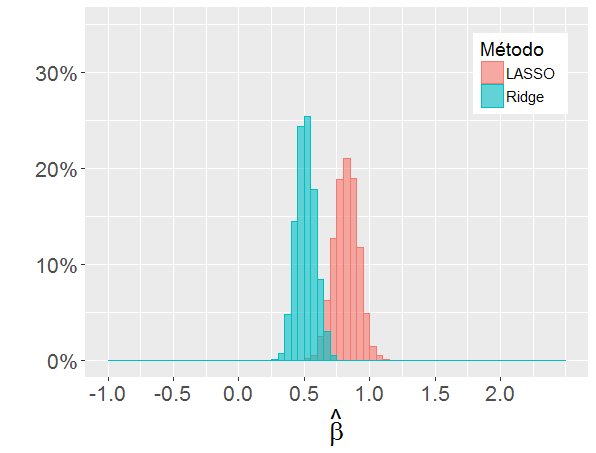
\includegraphics[width=7.95cm]{P 100 K 02 B1}
}
\subfloat[$k = 10$]{
  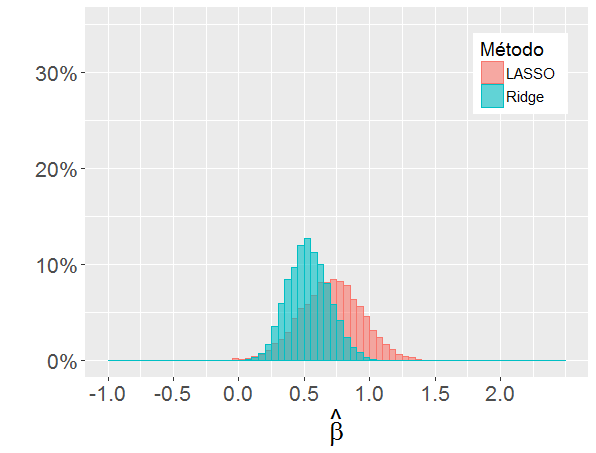
\includegraphics[width=7.95cm]{P 100 K 10 B1}
}
\hspace{0mm}
\subfloat[$k = 20$]{
  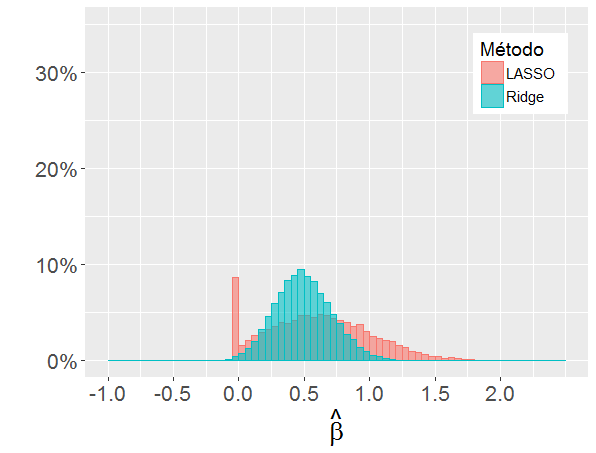
\includegraphics[width=7.95cm]{P 100 K 20 B1}
}
\subfloat[$k = 30 $]{
  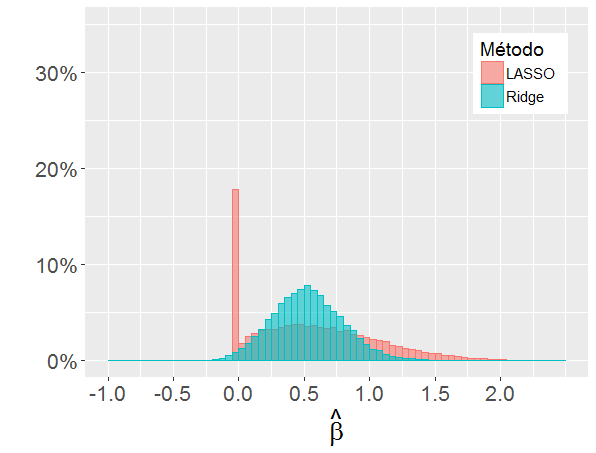
\includegraphics[width=7.95cm]{P 100 K 30 B1}
}
\hspace{0mm}
\subfloat[$k = 40$]{
  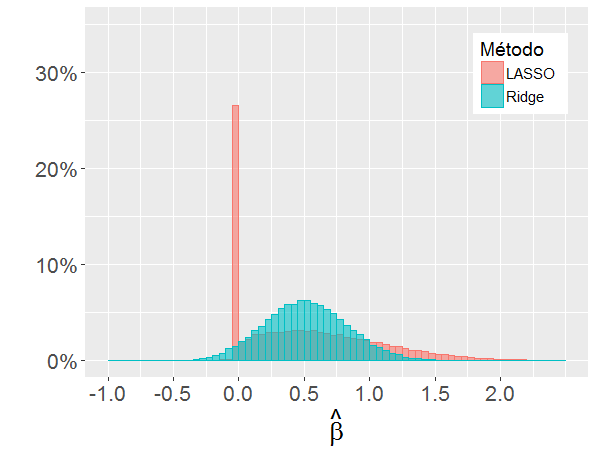
\includegraphics[width=7.95cm]{P 100 K 40 B1}
}
\subfloat[$k = 50$]{
  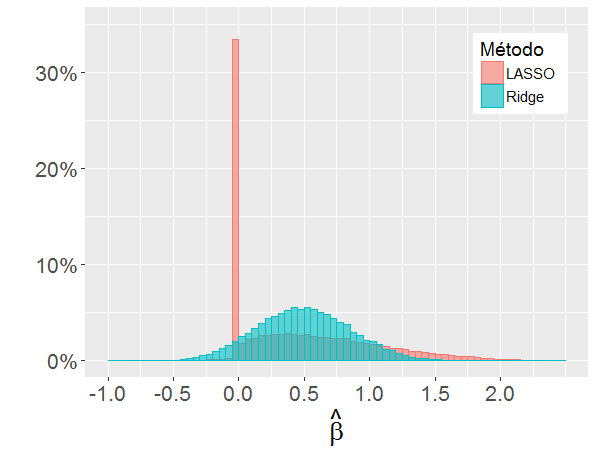
\includegraphics[width=7.95cm]{P 100 K 50 B1}
}
\caption{Distribución empírica de los estimadores $\hat{\beta}^{(1)}$ para variantes de $k$ \\ cuando $p=n=100$. Métodos \textit{Ridge} y LASSO}
\label{fig: P100 B1}
\end{figure}

\subsection*{Situación 2 ($p=2n=200$)}
En esta situación se restringe la comparación a los métodos \textit{Ridge} y LASSO por las propiedades de los estimadores MC señaladas en capítulos anteriores. En la Tabla \ref{tab: sit 2 B 1 med std} se muestran los promedios, desvíos estándares y coeficientes de variación a través de las 1.000 repeticiones.

\begin{table}[H]
\centering
\caption{Medidas características de las distribuciones de los estimadores $\hat{\beta}^{(1)}$ de cada método para variantes de $k$. Caso $p=2n=200$.}
\label{tab: sit 2 B 1 med std}
\footnotesize
\begin{tabular}{c|ccc|ccc}
 \multirow{3}{*}[-2em]{\textbf{k}} & \multicolumn{6}{c}{\textbf{Método}} \\[2ex]
 & \multicolumn{3}{c}{\textbf{Ridge}} & \multicolumn{3}{c}{\textbf{LASSO}} \\[2ex]
 & \scriptsize\makecell{\textbf{Promedio} \\ $\overline{\hat{\beta}}_{Ridge \hspace{0.05cm} \gamma}^{(1)}$} & \scriptsize\makecell{\textbf{Desvío} \\ \textbf{Estándar} \\ $S_{\hat{\beta}_{Ridge \hspace{0.05cm} \gamma}}^{(1)}$} & \scriptsize\textbf{CV(\%)} & \scriptsize\makecell{\textbf{Promedio} \\ $\overline{\hat{\beta}}_{LASSO \hspace{0.05cm} \gamma}^{(1)}$} & \scriptsize\makecell{\textbf{Desvío} \\ \textbf{Estándar} \\ $S_{\hat{\beta}_{LASSO \hspace{0.05cm} \gamma}}^{(1)}$} & \scriptsize\textbf{CV(\%)} \\ \hline
\textbf{2}   & 0,3152 & 0,0420 & \hspace{0.05cm} 13,32  & 0,7938 & 0,0937 & \hspace{0.05cm} 11,80  \\
\textbf{4}   & 0,2971 & 0,0657 & \hspace{0.05cm} 22,11  & 0,7242 & 0,1469 & \hspace{0.05cm} 20,28  \\
\textbf{6}   & 0,2911 & 0,0712 & \hspace{0.05cm} 24,46  & 0,6677 & 0,1795 & \hspace{0.05cm} 26,88  \\
\textbf{8}   & 0,3040 & 0,1108 & \hspace{0.05cm} 36,45  & 0,6146 & 0,2296 & \hspace{0.05cm} 37,36  \\
\textbf{10}  & 0,2944 & 0,1093 & \hspace{0.05cm} 37,13  & 0,5847 & 0,2570 & \hspace{0.05cm} 43,95  \\
\textbf{15}  & 0,3143 & 0,1294 & \hspace{0.05cm} 41,17  & 0,5265 & 0,3409 & \hspace{0.05cm} 64,75  \\
\textbf{20}  & 0,3228 & 0,1500 & \hspace{0.05cm} 46,47  & 0,4688 & 0,3714 & \hspace{0.05cm} 79,22  \\
\textbf{25}  & 0,3382 & 0,1653 & \hspace{0.05cm} 48,88  & 0,4377 & 0,4211 & \hspace{0.05cm} 96,21  \\
\textbf{30}  & 0,3229 & 0,1725 & \hspace{0.05cm} 53,42  & 0,3762 & 0,4345 & 115,50 \\
\textbf{35}  & 0,3202 & 0,1948 & \hspace{0.05cm} 60,84  & 0,3267 & 0,4338 & 132,78 \\
\textbf{40}  & 0,2818 & 0,2016 & \hspace{0.05cm} 71,54  & 0,2717 & 0,3975 & 146,30 \\
\textbf{45}  & 0,2580 & 0,2108 & \hspace{0.05cm} 81,71  & 0,2192 & 0,3676 & 167,70 \\
\textbf{50}  & 0,2632 & 0,2189 & \hspace{0.05cm} 83,17  & 0,2076 & 0,3642 & 175,43 \\
\textbf{60}  & 0,2851 & 0,2505 & \hspace{0.05cm} 87,86  & 0,2067 & 0,3815 & 184,57 \\
\textbf{70}  & 0,2927 & 0,2690 & \hspace{0.05cm} 91,90  & 0,2034 & 0,4006 & 196,95 \\
\textbf{80}  & 0,2911 & 0,2794 & \hspace{0.05cm} 95,98  & 0,1967 & 0,4117 & 209,30 \\
\textbf{90}  & 0,2872 & 0,2925 & 101,85 & 0,1721 & 0,4052 & 235,44 \\
\textbf{100} & 0,2835 & 0,3077 & 108,54 & 0,1625 & 0,4018 & 247,26
\end{tabular}
\end{table}

Al igual que en la Situación 1, los estimadores \textit{Ridge} son sesgados (Tabla \ref{tab: sit 2 B 1 med std}). Sin embargo, en este caso el sesgo es mayor, dado que los promedios son cercanos a 0,30 para todo $k$. Por otro lado, el sesgo de los estimadores LASSO nuevamente aumenta con $k$, observando sesgos mayores que en la Situación 1, sobre todo para valores de $k \geq 20$ aproximadamente.

Nuevamente, la variabilidad de los estimadores \textit{Ridge} y LASSO aumenta con $k$, observando que los coeficientes de variación LASSO son menores que los \textit{Ridge} cuando $k$ es pequeño y que esta relación se invierte cuando $k$ aumenta. 

Los coeficientes de variación LASSO de la Situación 2 son mucho mayores que los de la Situación 1 (Tabla \ref{tab: sit 1 B 1 med std}), sobre todo a partir de $k \geq 30$.

\begin{figure}[H]
\centering
\subfloat[$k = 2$]{
  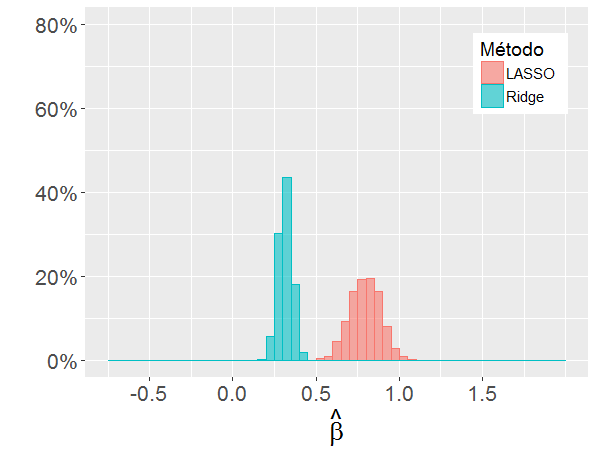
\includegraphics[width=7.95cm]{P 200 K 002 B1}
}
\subfloat[$k = 10$]{
  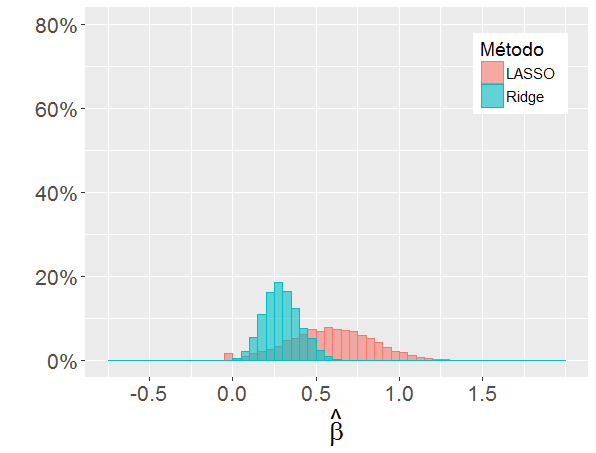
\includegraphics[width=7.95cm]{P 200 K 010 B1}
}
\hspace{0mm}
\subfloat[$k = 30$]{
  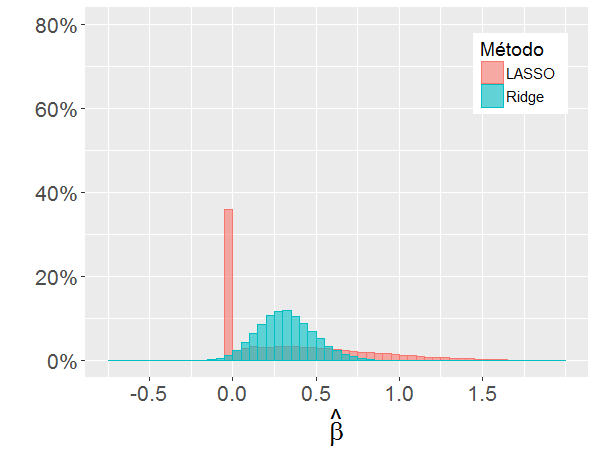
\includegraphics[width=7.95cm]{P 200 K 030 B1}
}
\subfloat[$k = 50 $]{
  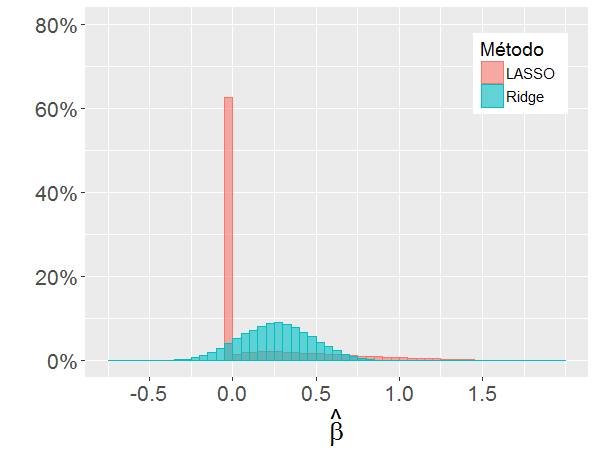
\includegraphics[width=7.95cm]{P 200 K 050 B1}
}
\hspace{0mm}
\subfloat[$k = 70$]{
  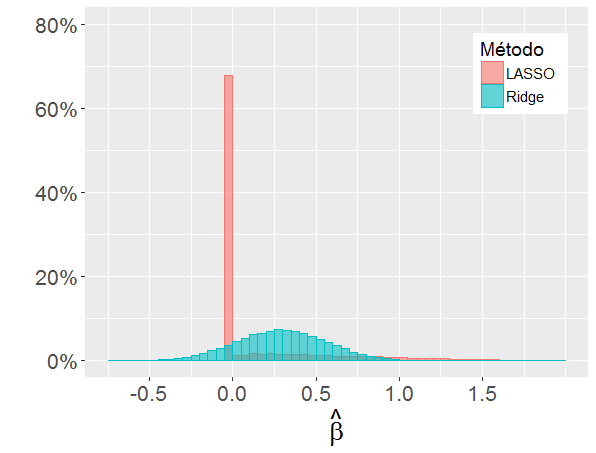
\includegraphics[width=7.95cm]{P 200 K 070 B1}
}
\subfloat[$k = 100$]{
  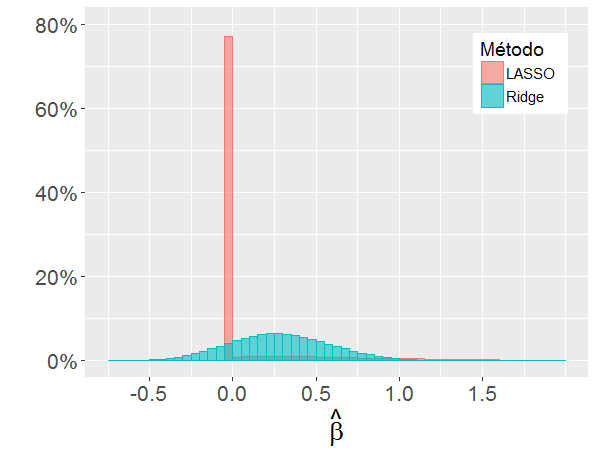
\includegraphics[width=7.95cm]{P 200 K 100 B1}
}
\caption{Distribución empírica de los estimadores $\hat{\beta}^{(1)}$ para variantes de $k$ \\ cuando $p=2n=200$}
\label{fig: P200 B1}
\end{figure}

En la Figura \ref{fig: P200 B1} se comparan las distribuciones de los estimadores $\hat{\beta}^{(1)}$ de los métodos \textit{Ridge} y LASSO. En esta figura vuelve a evidenciarse el comportamiento campanular de las distribuciones de los estimadores \textit{Ridge} para todo $k$. Este mismo comportamiento se observa para LASSO cuando $k$ es pequeño, pero a medida que $k$ aumenta, también lo hace la proporción de estimadores nulos, hecho que empeora el desempeño de este método.

\subsection*{Situación 3 ($p=4n=400$)}

\begin{table}[H]
\centering
\caption{Medidas características de las distribuciones de los estimadores $\hat{\beta}^{(1)}$ de cada método para variantes de $k$. Caso $p=4n=400$.}
\label{tab: sit 3 B 1 med std}
\footnotesize
\begin{tabular}{c|ccc|ccc}
 \multirow{3}{*}[-2em]{\textbf{k}} & \multicolumn{6}{c}{\textbf{Método}} \\[2ex]
 & \multicolumn{3}{c}{\textbf{Ridge}} & \multicolumn{3}{c}{\textbf{LASSO}} \\[2ex]
 & \scriptsize\makecell{\textbf{Promedio} \\ $\overline{\hat{\beta}}_{Ridge \hspace{0.05cm} \gamma}^{(1)}$} & \scriptsize\makecell{\textbf{Desvío} \\ \textbf{Estándar} \\ $S_{\hat{\beta}_{Ridge \hspace{0.05cm} \gamma}}^{(1)}$} & \scriptsize\textbf{CV(\%)} & \scriptsize\makecell{\textbf{Promedio} \\ $\overline{\hat{\beta}}_{LASSO \hspace{0.05cm} \gamma}^{(1)}$} & \scriptsize\makecell{\textbf{Desvío} \\ \textbf{Estándar} \\ $S_{\hat{\beta}_{LASSO \hspace{0.05cm} \gamma}}^{(1)}$} & \scriptsize\textbf{CV(\%)} \\ \hline
\textbf{2}   & 0,1444 & 0,0181 & \hspace{0.05cm} 12,53  & 0,7641 & 0,0951 & \hspace{0.05cm} 12,45 \\
\textbf{5}   & 0,1516 & 0,0355 & \hspace{0.05cm} 23,42 & 0,6402 & 0,1706 & \hspace{0.05cm} 26,65 \\
\textbf{10}  & 0,1497 & 0,0586 & \hspace{0.05cm} 39,14 & 0,4644 & 0,2688 & \hspace{0.05cm} 57,88  \\
\textbf{20}  & 0,1819 & 0,0874 & \hspace{0.05cm} 48,05 & 0,3109 & 0,3606 & 115,99 \\
\textbf{30}  & 0,1651 & 0,0950 & \hspace{0.05cm} 57,54 & 0,1871 & 0,3336 & 178,30 \\
\textbf{40}  & 0,1394 & 0,1080 & \hspace{0.05cm} 77,47 & 0,1042 & 0,2472 & 237,24 \\
\textbf{50}  & 0,1300 & 0,1143 & \hspace{0.05cm} 87,92 & 0,0732 & 0,2076 & 283,61 \\
\textbf{75}  & 0,1479 & 0,1420 & \hspace{0.05cm} 96,01 & 0,0643 & 0,2155 & 335,15 \\
\textbf{100} & 0,1603 & 0,1796 & 112,04 & 0,0503 & 0,2137 & 424,85 \\
\textbf{150} & 0,1730 & 0,2277 & 131,62 & 0,0405 & 0,2082 & 514,07 \\
\textbf{200} & 0,1764 & 0,2726 & 154,54 & 0,0419 & 0,2223 & 530,55
\end{tabular}
\end{table}

Nuevamente, los estimadores \textit{Ridge} son sesgados, en este caso con promedios cercanos a 0,15 para todo $k$ (Tabla \ref{tab: sit 3 B 1 med std}). La variabilidad de estos estimadores aumenta con $k$, siendo mayor que la observada en las Situaciones 1 y 2.

En la Situación 3, el sesgo de los estimadores LASSO es mayor que en las situaciones anteriores, y aumenta con mayor rapidez. A partir de $k\geq 50$ aproximadamente, se estabiliza. Al igual que lo observado para los estimadores \textit{Ridge}, los coeficientes de variación crecen con $k$, observándose valores mucho mayores que en los casos $p=n=100$ y $p=2n=200$.

A partir de $k=5$ aproximadamente, los coeficientes de variación de los estimadores \textit{Ridge} son menores que los de LASSO.

\begin{figure}[H]
\centering
\subfloat[$k = 2$]{
  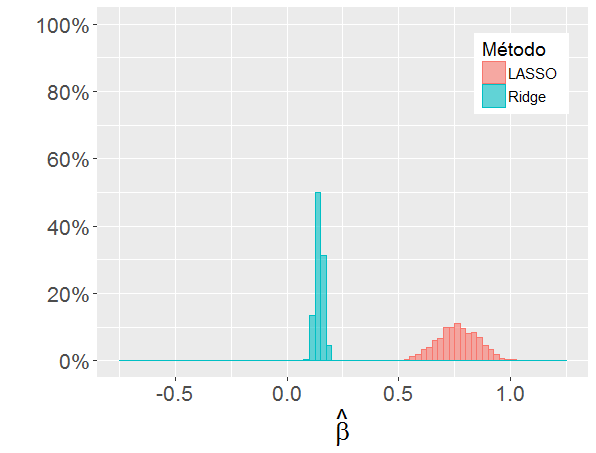
\includegraphics[width=7.95cm]{P 400 K 002 B1}
}
\subfloat[$k = 10$]{
  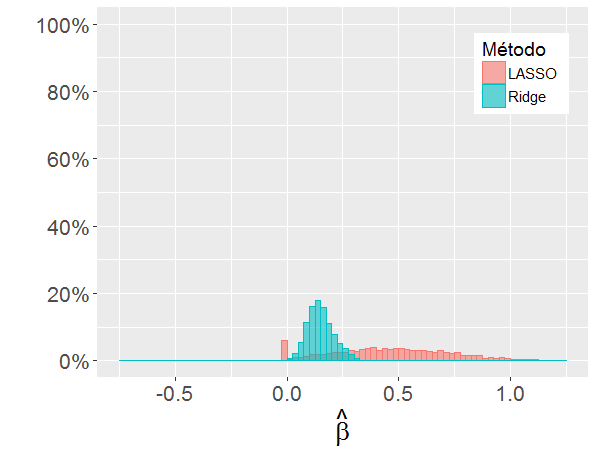
\includegraphics[width=7.95cm]{P 400 K 010 B1}
}
\hspace{0mm}
\subfloat[$k = 30$]{
  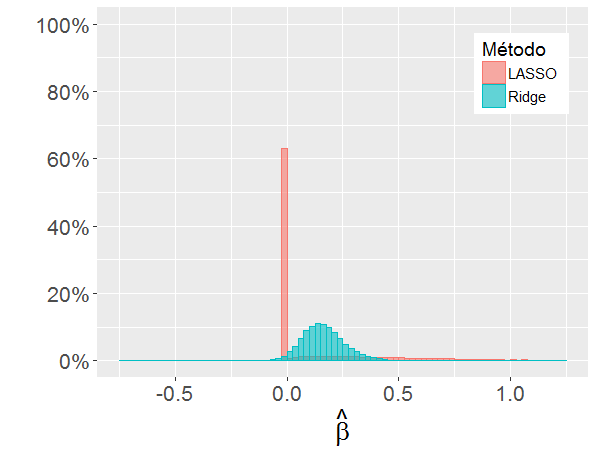
\includegraphics[width=7.95cm]{P 400 K 030 B1}
}
\subfloat[$k = 50 $]{
  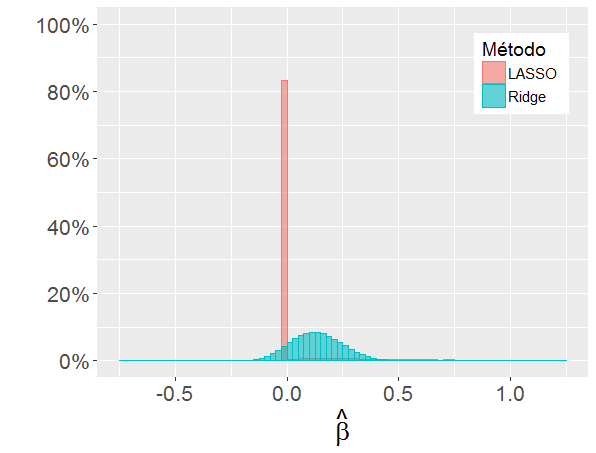
\includegraphics[width=7.95cm]{P 400 K 050 B1}
}
\hspace{0mm}
\subfloat[$k = 100$]{
  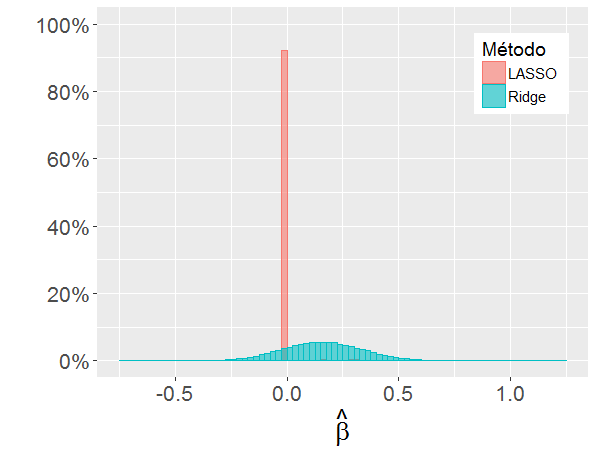
\includegraphics[width=7.95cm]{P 400 K 100 B1}
}
\subfloat[$k = 200$]{
  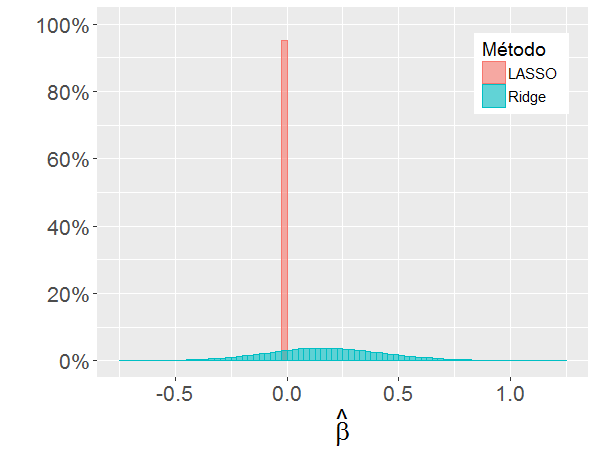
\includegraphics[width=7.95cm]{P 400 K 200 B1}
}
\caption{Distribución empírica de los estimadores $\hat{\beta}^{(1)}$ para variantes de $k$ \\ cuando $p=4n=400$}
\label{fig: P400 B1}
\end{figure}

En la Figura \ref{fig: P400 B1}, donde se comparan las distribuciones empíricas de los estimadores de $\beta=1$ de los métodos \textit{Ridge} y LASSO, se observan comportamientos idénticos a los observados en las Situaciones 1 y 2. Los estimadores \textit{Ridge} evidencian su conocida distribución Normal, y los LASSO presentan forma campanular hasta el momento en el que comienza a aumentar la proporción de estimaciones nulas. A partir de $k=30$ aproximadamente, la mayoría de las estimaciones LASSO son nulas, y este es el motivo por el cual disminuyen los desvíos estándares para este método en la Tabla \ref{tab: sit 3 B 1 med std}.

\section{Propiedades Distribucionales de Estimadores $\hat{\beta}^{(0)}$}
En esta Sección se comparan los promedios y desvíos estándares de los estimadores de los parámetros $\beta=0$ para cada método en cada escenario, agrupando escenarios por situación. A su vez, debido a la regularidad de los resultados obtenidos, se muestran gráficamente las distribuciones empíricas de los estimadores $\hat{\beta}^{(0)}$ para cada método sólo en algunos escenarios seleccionados. Los restantes pueden consultarse en el Anexo V.

\subsection*{Situación 1 ($p=n=100$)}
Con respecto a la propiedad de insesgamiento, la Tabla \ref{tab: sit 1 B 0 med std} corrobora que los estimadores MC tienen promedios muy cercanos a 0 para todo $k$. Lo mismo se observa para los estimadores de los métodos de regularización.

Las diferencias entre los métodos se observan en la variabilidad de sus estimaciones. Los desvíos estándares de los estimadores MC son severamente mayores que los de los métodos de regularización. Al comparar los desvíos de los estimadores \textit{Ridge} y LASSO, se observa que los de LASSO son siempre menores que los de \textit{Ridge}, y que esta diferencia disminuye a medida que $k$ aumenta.

\begin{table}[H]
\centering
\caption{Medidas características de las distribuciones de los estimadores $\hat{\beta}^{(0)}$ de cada método para variantes de $k$. Caso $p=n=100$.}
\label{tab: sit 1 B 0 med std}
\footnotesize
\begin{tabular}{c|cc|cc|cc}
\multirow{3}{*}[-2em]{\textbf{k}} & \multicolumn{6}{c}{\textbf{Método}} \\[2ex]
 & \multicolumn{2}{c}{\textbf{MC}} & \multicolumn{2}{c}{\textbf{Ridge}} & \multicolumn{2}{c}{\textbf{LASSO}} \\[2ex]
 & \scriptsize\makecell{\textbf{Promedio} \\ $\overline{\hat{\beta}}_{MC \hspace{0.05cm} \gamma}^{(0)}$} & \scriptsize\makecell{\textbf{Desvío} \\ \textbf{Estándar} \\ $S_{\hat{\beta}_{MC \hspace{0.05cm} \gamma}}^{(0)}$} & \scriptsize\makecell{\textbf{Promedio} \\ $\overline{\hat{\beta}}_{Ridge \hspace{0.05cm} \gamma}^{(0)}$} & \scriptsize\makecell{\textbf{Desvío} \\ \textbf{Estándar} \\ $S_{\hat{\beta}_{Ridge \hspace{0.05cm} \gamma}}^{(0)}$} & \scriptsize\makecell{\textbf{Promedio} \\ $\overline{\hat{\beta}}_{LASSO \hspace{0.05cm} \gamma}^{(0)}$} & \scriptsize\makecell{\textbf{Desvío} \\ \textbf{Estándar} \\ $S_{\hat{\beta}_{LASSO \hspace{0.05cm} \gamma}}^{(0)}$} \\ \hline
\textbf{2} & \hspace{0.005cm} 0,0008 & 0,6161 & -0,0063 & 0,0701 & -0,0005 & 0,0165 \\
\textbf{4} & \hspace{0.005cm} 0,0004 & 0,9163 & -0,0062 & 0,0997 & -0,0006 & 0,0337 \\
\textbf{6} & -0,0003 & 1,0949 & -0,0036 & 0,1230 & -0,0004 & 0,0516 \\
\textbf{8} & -0,0002 & 1,2753 & -0,0098 & 0,1410 & -0,0026 & 0,0729 \\
\textbf{10} & \hspace{0.005cm} 0,0007 & 1,4148 & -0,0133 & 0,1562 & -0,0034 & 0,0883 \\
\textbf{15} & \hspace{0.005cm} 0,0037 & 1,8268 & -0,0143 & 0,1909 & -0,0061 & 0,1330 \\
\textbf{20} & \hspace{0.005cm} 0,0048 & 2,1981 & -0,0207 & 0,2186 & -0,0109 & 0,1743 \\
\textbf{25} & \hspace{0.005cm} 0,0027 & 2,4424 & -0,0049 & 0,2530 & -0,0038 & 0,2126 \\
\textbf{30} & \hspace{0.005cm} 0,0035 & 2,6054 & -0,0140 & 0,2757 & -0,0119 & 0,2409 \\
\textbf{35} & \hspace{0.005cm} 0,0054 & 2,9075 & -0,0052 & 0,2957 & -0,0069 & 0,2637 \\
\textbf{40} & \hspace{0.005cm} 0,0119 & 2,9093 & \hspace{0.005cm} 0,0027 & 0,3188 & \hspace{0.005cm} 0,0003 & 0,2852 \\
\textbf{45} & \hspace{0.005cm} 0,0118 & 2,9018 & \hspace{0.005cm} 0,0259 & 0,3428 & \hspace{0.005cm} 0,0169 & 0,3219 \\
\textbf{50} & \hspace{0.005cm} 0,0135 & 3,1190 & \hspace{0.005cm} 0,0180 & 0,3600 & \hspace{0.005cm} 0,0076 & 0,3356
\end{tabular}
\end{table}

En la Figura \ref{fig: P100 B0 MC}, donde se comparan las distribuciones de los estimadores de los parámetros $\beta=0$ obtenidos por el ajuste mínimo-cuadrático, regresión \textit{Ridge} y regresión LASSO, se evidencia lo explicitado a partir de los desvíos estándares (Tabla \ref{tab: sit 1 B 0 med std}). La distribución de los estimadores MC es mucho más dispersa que la de los métodos de regularización. En esta figura se observa que los estimadores \textit{Ridge} muestran distribuciones campanulares para todo $k$.

Dada la gran variabilidad de los estimadores MC en relación a la de los métodos de regularización, la Figura \ref{fig: P100 B0} repite estas distribuciones sólo para los estimadores de los métodos \textit{Ridge} y LASSO. En ella se observa mejor cómo la variabilidad de ambos métodos aumenta con $k$. Una consecuencia de esto es la disminución de la proporción de estimadores LASSO que son nulos a medida que $k$ aumenta.

\begin{figure}[H]
\centering
\subfloat[$k = 2$]{
  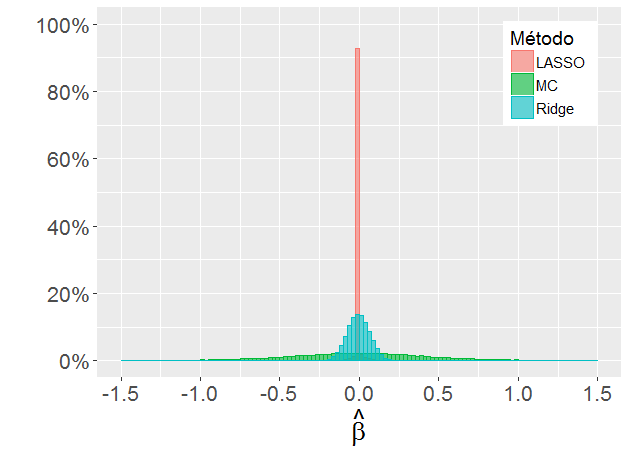
\includegraphics[width=7.95cm]{P 100 K 02 B0 MC}
}
\subfloat[$k = 10$]{
  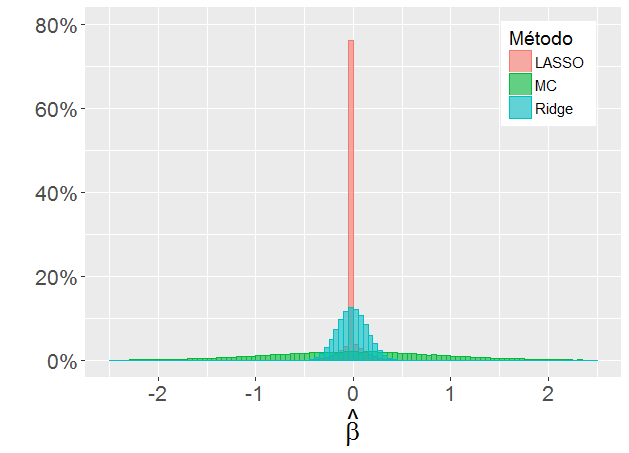
\includegraphics[width=7.95cm]{P 100 K 10 B0 MC}
}
\hspace{0mm}
\subfloat[$k = 20$]{
  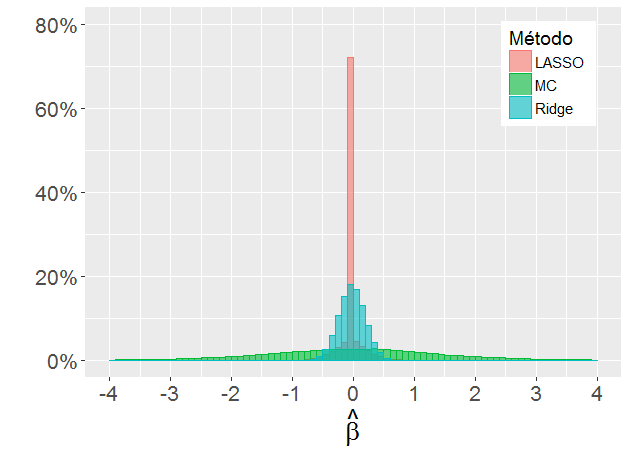
\includegraphics[width=7.95cm]{P 100 K 20 B0 MC}
}
\subfloat[$k = 30 $]{
  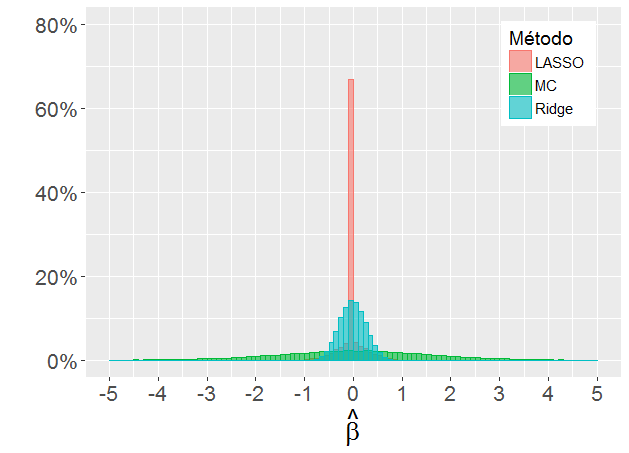
\includegraphics[width=7.95cm]{P 100 K 30 B0 MC}
}
\hspace{0mm}
\subfloat[$k = 40$]{
  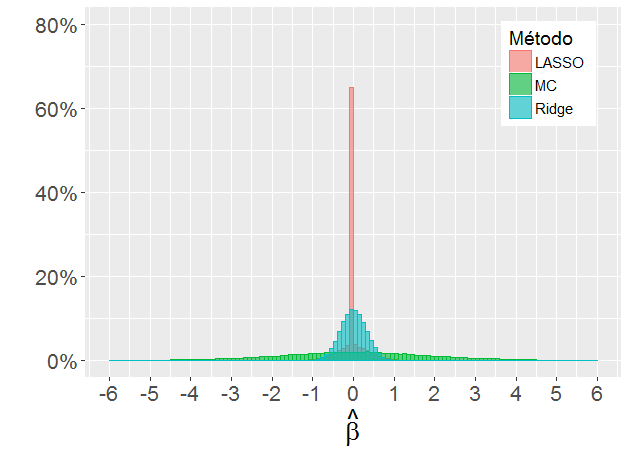
\includegraphics[width=7.95cm]{P 100 K 40 B0 MC}
}
\subfloat[$k = 50$]{
  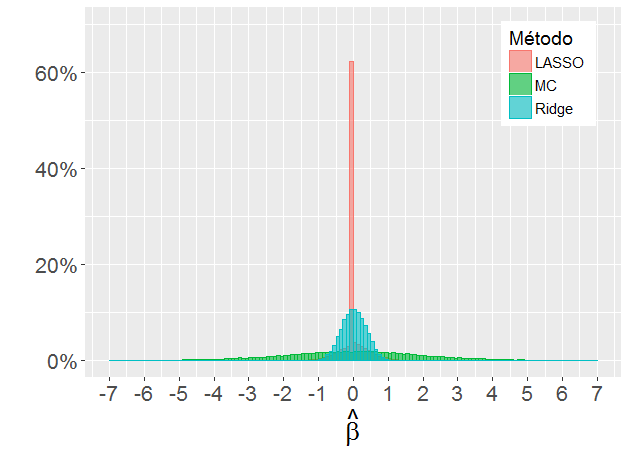
\includegraphics[width=7.95cm]{P 100 K 50 B0 MC}
}
\caption{Distribución empírica de los estimadores $\hat{\beta}^{(0)}$ para variantes de $k$ \\ cuando $p=n=100$. Métodos MC, \textit{Ridge} y LASSO}
\label{fig: P100 B0 MC}
\end{figure}

\begin{figure}[H]
\centering
\subfloat[$k = 2$]{
  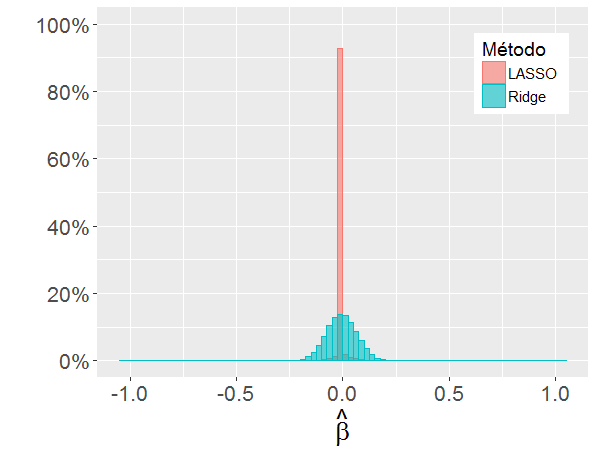
\includegraphics[width=7.95cm]{P 100 K 02 B0}
}
\subfloat[$k = 10$]{
  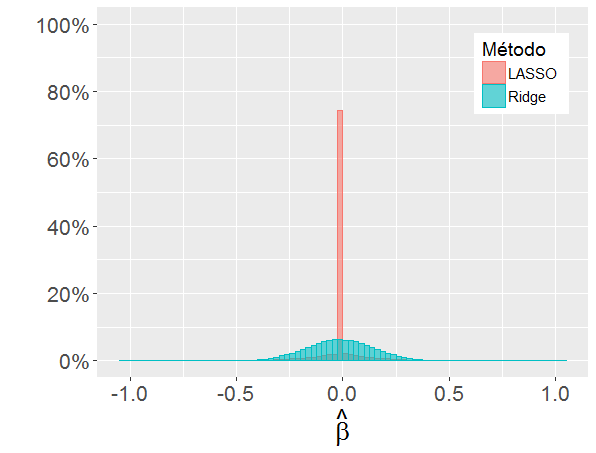
\includegraphics[width=7.95cm]{P 100 K 10 B0}
}
\hspace{0mm}
\subfloat[$k = 20$]{
  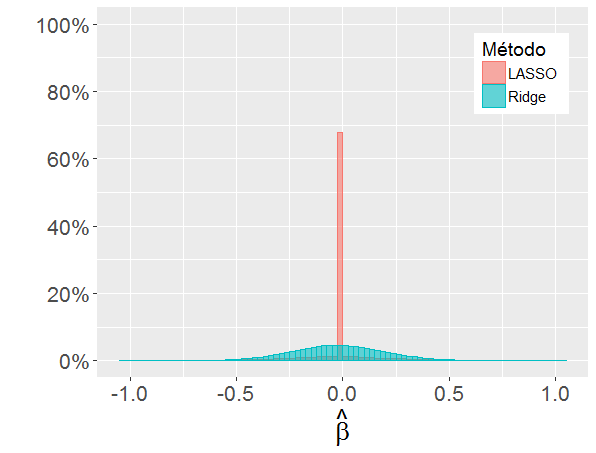
\includegraphics[width=7.95cm]{P 100 K 20 B0}
}
\subfloat[$k = 30 $]{
  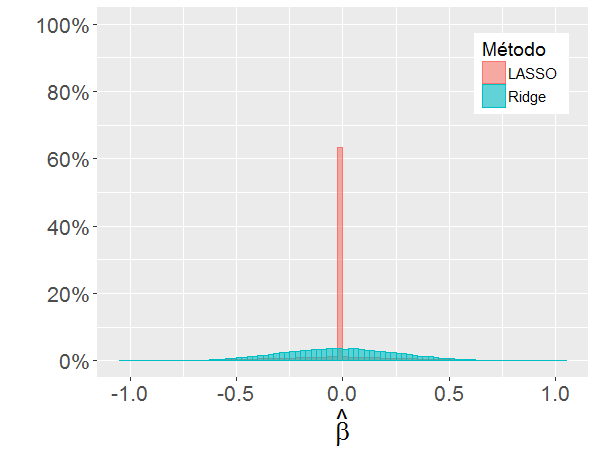
\includegraphics[width=7.95cm]{P 100 K 30 B0}
}
\hspace{0mm}
\subfloat[$k = 40$]{
  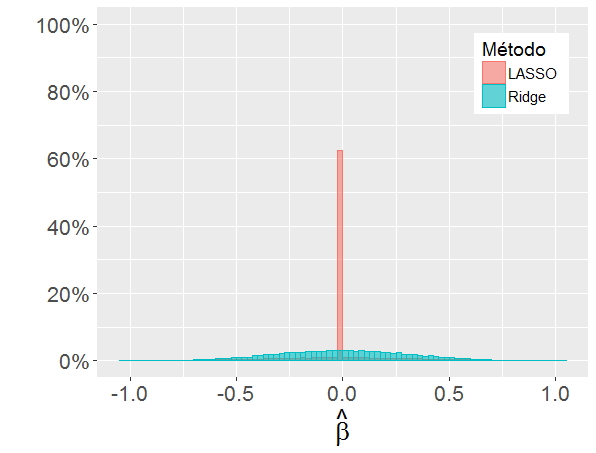
\includegraphics[width=7.95cm]{P 100 K 40 B0}
}
\subfloat[$k = 50$]{
  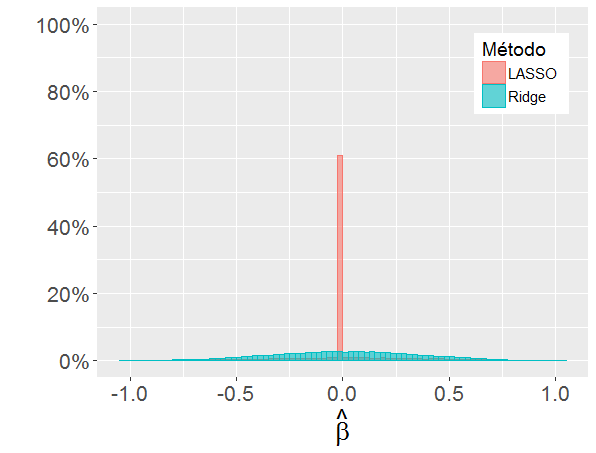
\includegraphics[width=7.95cm]{P 100 K 50 B0}
}
\caption{Distribución empírica de los estimadores $\hat{\beta}^{(0)}$ para variantes de $k$ \\ cuando $p=n=100$. Métodos \textit{Ridge} y LASSO}
\label{fig: P100 B0}
\end{figure}


\subsection*{Situación 2 ($p=2n=200$)}

\begin{table}[H]
\centering
\caption{Medidas características de las distribuciones de los estimadores $\hat{\beta}^{(0)}$ de cada método para variantes de $k$. Caso $p=2n=200$.}
\label{tab: sit 2 B 0 med std}
\footnotesize
\begin{tabular}{c|cc|cc}
\multirow{3}{*}[-2em]{\textbf{k}} & \multicolumn{4}{c}{\textbf{Método}} \\[2ex]
 & \multicolumn{2}{c}{\textbf{Ridge}} & \multicolumn{2}{c}{\textbf{LASSO}} \\[2ex]
 & \scriptsize\makecell{\textbf{Promedio} \\ $\overline{\hat{\beta}}_{Ridge \hspace{0.05cm} \gamma}^{(0)}$} & \scriptsize\makecell{\textbf{Desvío} \\ \textbf{Estándar} \\ $S_{\hat{\beta}_{Ridge \hspace{0.05cm} \gamma}}^{(0)}$} & \scriptsize\makecell{\textbf{Promedio} \\ $\overline{\hat{\beta}}_{LASSO \hspace{0.05cm} \gamma}^{(0)}$} & \scriptsize\makecell{\textbf{Desvío} \\ \textbf{Estándar} \\ $S_{\hat{\beta}_{LASSO \hspace{0.05cm} \gamma}}^{(0)}$} \\ \hline
\textbf{2} & -0,0011 & 0,0471 & -0,0001 & 0,0121 \\
\textbf{4} & \hspace{0.005cm} 0,0001 & 0,0652 & \hspace{0.005cm} 0,0000 & 0,0248 \\
\textbf{6} & \hspace{0.005cm} 0,0018 & 0,0801 & \hspace{0.005cm} 0,0004 & 0,0415 \\
\textbf{8} & \hspace{0.005cm} 0,0023 & 0,0931 & \hspace{0.005cm} 0,0009 & 0,0622 \\
\textbf{10} & -0,0010 & 0,1026 & \hspace{0.005cm} 0,0005 & 0,0734 \\
\textbf{15} & -0,0021 & 0,1279 & \hspace{0.005cm} 0,0000 & 0,1041 \\
\textbf{20} & \hspace{0.005cm} 0,0023 & 0,1482 & \hspace{0.005cm} 0,0014 & 0,1264 \\
\textbf{25} & \hspace{0.005cm} 0,0066 & 0,1719 & \hspace{0.005cm} 0,0041 & 0,1549 \\
\textbf{30} & \hspace{0.005cm} 0,0036 & 0,1868 & -0,0008 & 0,1612 \\
\textbf{35} & -0,0004 & 0,1975 & -0,0035 & 0,1575 \\
\textbf{40} & \hspace{0.005cm} 0,0051 & 0,2012 & -0,0037 & 0,1680 \\
\textbf{45} & \hspace{0.005cm} 0,0124 & 0,2071 & -0,0012 & 0,1775 \\
\textbf{50} & \hspace{0.005cm} 0,0059 & 0,2198 & -0,0055 & 0,1715 \\
\textbf{60} & \hspace{0.005cm} 0,0136 & 0,2473 & -0,0011 & 0,1872 \\
\textbf{70} & \hspace{0.005cm} 0,0109 & 0,2719 & -0,0066 & 0,2055 \\
\textbf{80} & \hspace{0.005cm} 0,0127 & 0,2894 & -0,0041 & 0,2239 \\
\textbf{90} & \hspace{0.005cm} 0,0158 & 0,3087 & -0,0033 & 0,2341 \\
\textbf{100} & \hspace{0.005cm} 0,0225 & 0,3260 & \hspace{0.005cm} 0,0018 & 0,2451
\end{tabular}
\end{table}

Al igual que en el caso $p=n=100$, los promedios de los estimadores \textit{Ridge} y LASSO son cercanos a 0 (Tabla \ref{tab: sit 2 B 0 med std}). Los desvíos estándares de los estimadores \textit{Ridge} son siempre mayores que los de LASSO, y esta diferencia disminuye a medida que $k$ aumenta.

En la Figura \ref{fig: P200 B0} se comparan las distribuciones de los estimadores $\hat{\beta}^{(0)}$ de los métodos \textit{Ridge} y LASSO. En ella se observa el comportamiento campanular de la distribución de los estimadores \textit{Ridge}, el cual se hace menos visible para valores de $k$ grandes debido al aumento de su variabilidad y por haber mantenido la escala para dibujar simultáneamente las distribuciones para ambos métodos. Con respecto a estos últimos, se observa que el porcentaje de estimaciones nulas disminuye con $k$ hasta $k=30$ aproximadamente, y a partir de ese valor el mismo aumenta levemente con $k$. De todos modos, esta proporción se mantiene alrededor del $85\%$ en todo momento.

\begin{figure}[H]
\centering
\subfloat[$k = 2$]{
  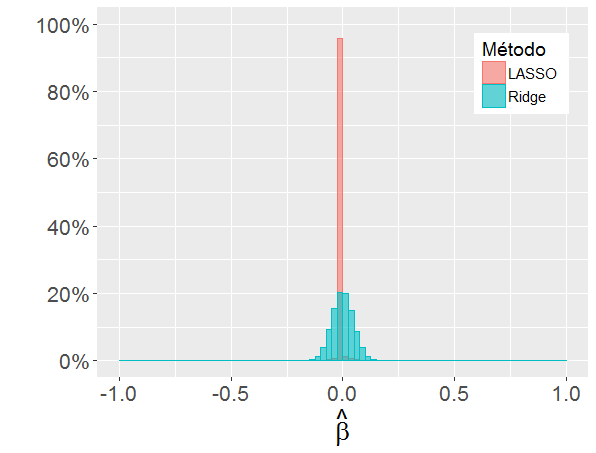
\includegraphics[width=7.95cm]{P 200 K 002 B0}
}
\subfloat[$k = 10$]{
  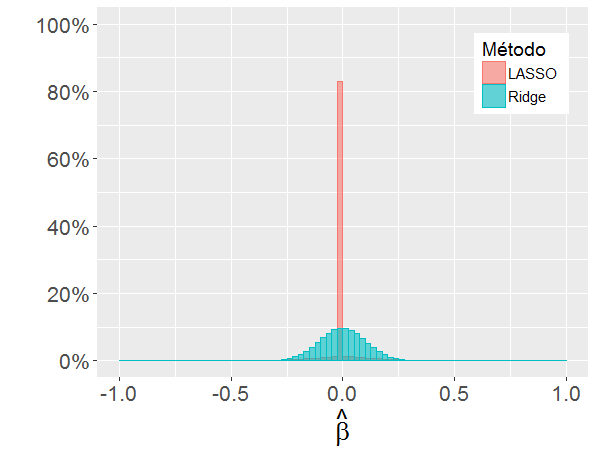
\includegraphics[width=7.95cm]{P 200 K 010 B0}
}
\hspace{0mm}
\subfloat[$k = 30$]{
  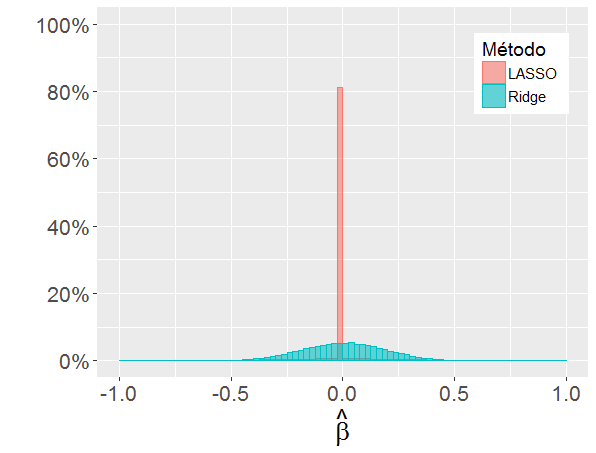
\includegraphics[width=7.95cm]{P 200 K 030 B0}
}
\subfloat[$k = 50 $]{
  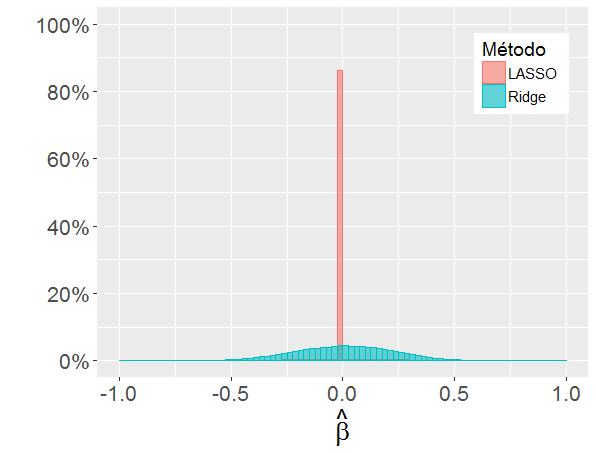
\includegraphics[width=7.95cm]{P 200 K 050 B0}
}
\hspace{0mm}
\subfloat[$k = 70$]{
  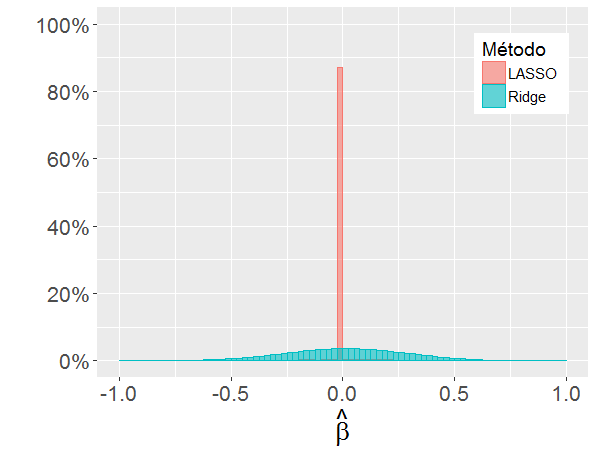
\includegraphics[width=7.95cm]{P 200 K 070 B0}
}
\subfloat[$k = 100$]{
  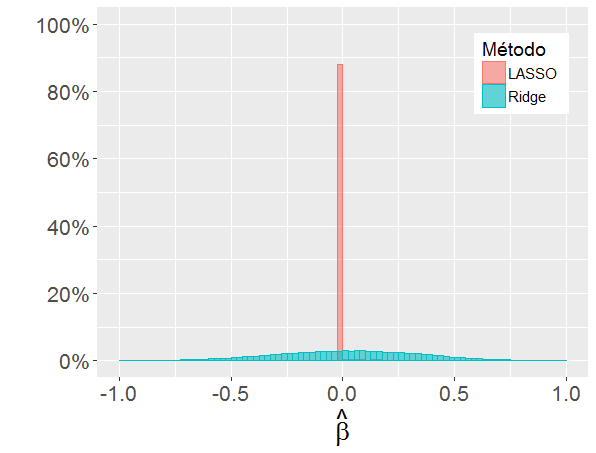
\includegraphics[width=7.95cm]{P 200 K 100 B0}
}
\caption{Distribución empírica de los estimadores $\hat{\beta}^{(0)}$ para variantes de $k$ \\ cuando $p=2n=200$}
\label{fig: P200 B0}
\end{figure}

\subsection*{Situación 3 ($p=4n=400$)}

\begin{table}[H]
\centering
\caption{Promedio y desvío estándar de las distribuciones de los estimadores de parámetros $\beta=0$ para cada método en cada escenario de la Situación 3}
\label{tab: sit 3 B 0 med std}
\footnotesize
\begin{tabular}{c|cc|cc}
\multirow{3}{*}[-2em]{\textbf{k}} & \multicolumn{4}{c}{\textbf{Método}} \\[2ex]
 & \multicolumn{2}{c}{\textbf{Ridge}} & \multicolumn{2}{c}{\textbf{LASSO}} \\[2ex]
 & \scriptsize\makecell{\textbf{Promedio} \\ $\overline{\hat{\beta}}_{Ridge \hspace{0.05cm} \gamma}^{(0)}$} & \scriptsize\makecell{\textbf{Desvío} \\ \textbf{Estándar} \\ $S_{\hat{\beta}_{Ridge \hspace{0.05cm} \gamma}}^{(0)}$} & \scriptsize\makecell{\textbf{Promedio} \\ $\overline{\hat{\beta}}_{LASSO \hspace{0.05cm} \gamma}^{(0)}$} & \scriptsize\makecell{\textbf{Desvío} \\ \textbf{Estándar} \\ $S_{\hat{\beta}_{LASSO \hspace{0.05cm} \gamma}}^{(0)}$} \\ \hline
\textbf{2} & -0,0001 & 0,0247 & \hspace{0.005cm} 0,0001 & 0,0087 \\
\textbf{5} & \hspace{0.005cm} 0,0019 & 0,0402 & \hspace{0.005cm} 0,0004 & 0,0251 \\
\textbf{10} & \hspace{0.005cm} 0,0001 & 0,0564 & \hspace{0.005cm} 0,0011 & 0,0567 \\
\textbf{20} & \hspace{0.005cm} 0,0012 & 0,0871 & \hspace{0.005cm} 0,0024 & 0,0806 \\
\textbf{30} & \hspace{0.005cm} 0,0010 & 0,1030 & \hspace{0.005cm} 0,0002 & 0,0832 \\
\textbf{40} & \hspace{0.005cm} 0,0002 & 0,1091 & -0,0015 & 0,0876 \\
\textbf{50} & -0,0006 & 0,1184 & -0,0018 & 0,0854 \\
\textbf{75} & -0,0014 & 0,1543 & -0,0028 & 0,0973 \\
\textbf{100} & -0,0022 & 0,1841 & -0,0027 & 0,0898 \\
\textbf{150} & -0,0040 & 0,2328 & -0,0011 & 0,0946 \\
\textbf{200} & -0,0104 & 0,2668 & -0,0005 & 0,0926
\end{tabular}
\end{table}

Nuevamente, los promedios de los estimadores \textit{Ridge} y LASSO son cercanos a 0 para todo valor de $k$ (Tabla \ref{tab: sit 3 B 1 med std}). Los desvíos estándares de los estimadores \textit{Ridge} aumentan con $k$, mientras que los de LASSO aumentan hasta $k=20$ aproximadamente, manteniéndose relativamente constantes a partir de dicho valor. Se observa que la variabilidad de los estimadores LASSO es siempre menor que la de los \textit{Ridge}, repitiendo el comportamiento de las Situaciones 1 y 2.

En la Figura \ref{fig: P400 B0}, donde se presentan las distribuciones de los estimadores $\hat{\beta}^{(0)}$ para cada método, se observa que los estimadores \textit{Ridge} se comportan igual que en el caso $p=2n=200$. En la Situación 3, la proporción de estimaciones LASSO nulas disminuye hasta $k=10$ aproximadamente, y luego aumenta con $k$, manteniendo proporciones cercanas a 1, siendo este el motivo por el cual la variabilidad de las estimaciones LASSO se estabiliza para valores de $k$ grandes. 

\begin{figure}[H]
\centering
\subfloat[$k = 2$]{
  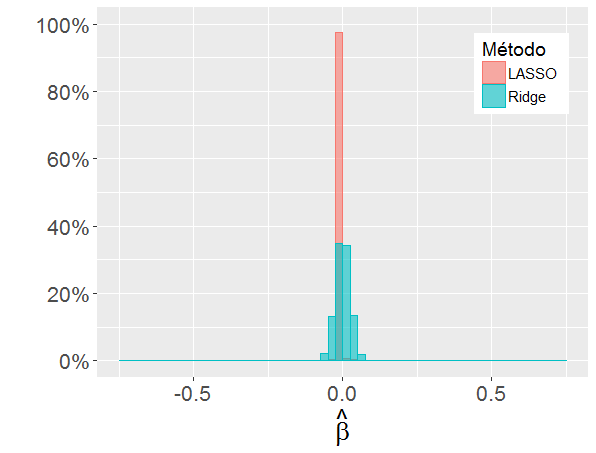
\includegraphics[width=7.95cm]{P 400 K 002 B0}
}
\subfloat[$k = 10$]{
  \includegraphics[width=7.95cm]{P 400 K 010 B0}
}
\hspace{0mm}
\subfloat[$k = 30$]{
  \includegraphics[width=7.95cm]{P 400 K 030 B0}
}
\subfloat[$k = 50 $]{
  \includegraphics[width=7.95cm]{P 400 K 050 B0}
}
\hspace{0mm}
\subfloat[$k = 100$]{
  \includegraphics[width=7.95cm]{P 400 K 100 B0}
}
\subfloat[$k = 200$]{
  \includegraphics[width=7.95cm]{P 400 K 200 B0}
}
\caption{Distribución empírica de los estimadores $\hat{\beta}^{(0)}$ para variantes de $k$ \\ cuando $p=4n=400$}
\label{fig: P400 B0}
\end{figure}

\section{Medidas Específicas de Estimadores LASSO}
En esta Sección se estudia la capacidad de los estimadores LASSO de obtener estimaciones nulas, tanto para la situación no deseable donde el parámetro a estimar es $\beta = 1$, como para la situación deseable donde $\beta = 0$. Los resultados se presentan para las variantes de $k$, separados por situación. 

\subsection*{Situación 1 ($p=n=100$)}

\begin{table}[H]
\centering
\caption{Medidas específicas calculadas para los estimadores LASSO. \\ Caso $p=n=100$.}
\label{tab: sit 1 lasso measures}
\footnotesize
\begin{tabular}{c|c|c}
\textbf{k} & $\hat{\beta}^{(0)} = 0$ (\%) & $\hat{\beta}^{(1)} = 0$ (\%) \\
\hline
\textbf{2} & 90,59 & \hspace{0.07cm} 0,00 \\
\textbf{4} & 85,03 & \hspace{0.07cm} 0,00 \\
\textbf{6} & 79,34 & \hspace{0.07cm} 0,00 \\
\textbf{8} & 74,23 & \hspace{0.07cm} 0,01 \\
\textbf{10} & 71,95 & \hspace{0.07cm} 0,27 \\
\textbf{15} & 68,20 & \hspace{0.07cm} 2,87 \\
\textbf{20} & 66,25 & \hspace{0.07cm} 8,65 \\
\textbf{25} & 62,83 & 12,33 \\
\textbf{30} & 61,86 & 17,76 \\
\textbf{35} & 62,66 & 23,79 \\
\textbf{40} & 60,76 & 26,36 \\
\textbf{45} & 56,61 & 29,77 \\
\textbf{50} & 58,57 & 33,04
\end{tabular}
\end{table}

El porcentaje de $\hat{\beta}^{(0)}$ que son nulos disminuye a medida que $k$ aumenta (Tabla \ref{tab: sit 1 lasso measures}). Esto está relacionado con el aumento en la variabilidad de las estimaciones presente en los resultados de la Tabla \ref{tab: sit 1 B 0 med std}. Por otro lado, el porcentaje de $\hat{\beta}^{(1)}$ que son nulos aumenta con $k$, lo cual muestra un mal desempeño de los estimadores LASSO cuando $k$ es grande.

\subsection*{Situación 2 ($p=2n=200$)}

\begin{table}[H]
\centering
\caption{Medidas específicas calculadas para los estimadores LASSO. \\ Caso $p=2n=200$.}
\label{tab: sit 2 lasso measures}
\footnotesize
\begin{tabular}{c|c|c}
\textbf{k} & $\hat{\beta}^{(0)} = 0$ (\%) & $\hat{\beta}^{(1)} = 0$ (\%) \\
\hline
\textbf{2} & 94,45 & \hspace{0.07cm} 0,00 \\
\textbf{4} & 91,10 & \hspace{0.07cm} 0,00 \\
\textbf{6} & 86,83 & \hspace{0.07cm} 0,02 \\
\textbf{8} & 82,49 & \hspace{0.07cm} 0,73 \\
\textbf{10} & 81,54 & \hspace{0.07cm} 1,80 \\
\textbf{15} & 80,17 & \hspace{0.07cm} 8,66 \\
\textbf{20} & 80,55 & 19,21 \\
\textbf{25} & 78,70 & 25,43 \\
\textbf{30} & 80,30 & 35,77 \\
\textbf{35} & 83,40 & 45,14 \\
\textbf{40} & 83,39 & 51,29 \\
\textbf{45} & 83,46 & 59,00 \\
\textbf{50} & 85,32 & 62,30 \\
\textbf{60} & 85,87 & 64,45 \\
\textbf{70} & 85,96 & 67,33 \\
\textbf{80} & 86,35 & 70,01 \\
\textbf{90} & 86,81 & 75,06 \\
\textbf{100} & 86,22 & 76,47
\end{tabular}
\end{table}

En este caso, el porcentaje de parámetros nulos estimados por cero por LASSO disminuye hasta $k=25$ y luego aumenta con $k$, manteniéndose siempre en valores altos (\ref{tab: sit 2 lasso measures}). Por otro lado, el porcentaje de parámetros $\beta=1$ cuyas estimaciones son nulas aumenta con $k$, observando porcentajes mucho mayores que en el caso $p=n=100$.

\subsection*{Situación 3 ($p=4n=400$)}

\begin{table}[H]
\centering
\caption{Medidas específicas calculadas para los estimadores LASSO. \\ Caso $p=4n=400$.}
\label{tab: sit 3 lasso measures}
\footnotesize
\begin{tabular}{c|c|c}
\textbf{k} & $\hat{\beta}^{(0)} = 0$ (\%) & $\hat{\beta}^{(1)} = 0$ (\%) \\
\hline
\textbf{2} & 96,90 & \hspace{0.07cm} 0,00 \\
\textbf{5} & 93,23 & \hspace{0.07cm} 0,02 \\
\textbf{10} & 89,04 & \hspace{0.07cm} 6,14 \\
\textbf{20} & 91,07 & 37,58 \\
\textbf{30} & 92,92 & 61,83 \\
\textbf{40} & 94,59 & 76,43 \\
\textbf{50} & 95,37 & 83,01 \\
\textbf{75} & 95,78 & 87,15 \\
\textbf{100} & 96,90 & 91,33 \\
\textbf{150} & 97,65 & 94,14 \\
\textbf{200} & 97,92 & 94,20
\end{tabular}
\end{table}

Nuevamente, se observa que el porcentaje de $\hat{\beta}^{(0)} = 0$ disminuye con $k$ para valores de $k$ pequeños, en este caso hasta $k=10$ aproximadamente, y partir de dicho valor ese porcentaje aumenta con $k$ (Tabla \ref{tab: sit 3 lasso measures}). Se observan porcentajes muy altos en todo momento, mayores que los de la Tabla \ref{tab: sit 2 lasso measures}. Como en las Situaciones 1 y 2, el porcentaje de $\hat{\beta}^{(1)} = 0$ aumenta con $k$, observando en este caso porcentajes mucho más elevados que en las otras dos situaciones. A partir de $k=50$ aproximadamente, casi la totalidad de las estimaciones LASSO son nulas, tanto aquellas que estiman parámetros nulos como las que estiman parámetros no nulos.

\chapter{Conclusiones}
El trabajo desarrollado se aboca a una problemática frecuente en el contexto actual del análisis de datos, estudiando modelos estimados a partir de bases de datos de grandes dimensiones. El uso de modelos en estadística es una herramienta utilizada con mucha frecuencia por la riqueza que brinda al analizar relaciones entre variables y la posibilidad de predecir ciertas variables de interés bajo condiciones particulares. Clásicamente, cuando se plantean modelos lineales, la estimación de sus parámetros se hace bajo el método de mínimos cuadrados, el cual tiene excelentes propiedades cuando el número de observaciones es considerablemente mayor que el de parámetros a estimar. Las actuales condiciones de recolección de datos, facilitada por el uso de mecanismos automatizados, implican frecuentemente que ésta condición no se verifique y aparezca la necesidad de estimar muchos parámetros con una cantidad pequeña de observaciones. Para estas situaciones se han propuesto métodos alternativos de estimación, dos de los cuales son objeto de un análisis más profundo en esta tesina: las regresiones \textit{Ridge} y LASSO. Estas técnicas son métodos de regularización que imponen restricciones adicionales para la estimación de los parámetros.

En este trabajo se hace una síntesis de los métodos de estimación de los parámetros de los modelos lineales tanto en el contexto clásico (mínimos cuadrados) como los métodos más novedosos, aplicables en el contexto de grandes dimensiones (selección del mejor subconjunto, regresión \textit{Ridge}, regresión LASSO y red elástica). Sólo se considera la situación de variables predictivas y de respuesta continuas, señalando los criterios de optimización que requiere cada método, las propiedades de los estimadores, cómo obtener predicciones y su variabilidad, y algunos métodos computacionales imprescindibles para la aplicación de la regresión LASSO.
 
En particular, mínimos cuadrados no tiene solución única cuando el número de variables explicativas es mayor que el número de observaciones, motivo por el cual es necesario recurrir a métodos como los de regularización. En estos últimos, la solución depende de la elección de un parámetro de suavizado, dando lugar a un camino de soluciones. De todas las soluciones calculadas para algunas variantes de este parámetro previamente establecidas, se elige la mejor de acuerdo a algún criterio, como por ejemplo, minimización del ECM, recomendándose el uso de validación cruzada. Previo a la aplicación de los métodos de regularización resulta conveniente estandarizar los predictores, para evitar que la elección del parámetro de suavizado se vea influenciada por la escala de los mismos. El estimador \textit{Ridge} puede ser calculado unívocamente y siempre tiene una forma cerrada para su cálculo. LASSO admite solución en forma cerrada únicamente cuando la matriz de predictores es ortogonal. Cuando este no es el caso, obtener el estimador LASSO constituye un problema de programación cuadrático, cuya solución puede ser aproximada eficientemente. En este trabajo también se mencionan características particulares de los problemas de optimización planteados por los métodos \textit{Ridge} y LASSO y se hace una breve descripción de un software libre que puede ser utilizado para implementar la estimación del método LASSO, el cual es intensivo computacionalmente.

En esta tesina se plantea un estudio por simulación diseñado para mostrar las propiedades de estos métodos frente a distintos contextos de volumen de información disponible respecto de la cantidad de parámetros a estimar. Se definen tres situaciones distintas, una donde el número de observaciones es igual al número de parámetros y dos en las cuales hay el doble y el cuádruple de parámetros respecto del número de observaciones. En cada una de las situaciones se construyen distintos modelos variando el grado de esparcimiento ($k$) de los mismos, siendo $k$ el número de parámetros no nulos del modelo. Sin pérdida de generalidad, los parámetros no nulos se fijan en uno. A fin de establecer una comparación entre los métodos se identificaron medidas globales de eficiencia, a saber: ECM de los modelos, variabilidad y sesgo de los estimadores de los parámetros separando en dos casos, nulos y no nulos, forma de su distribución empírica y capacidad del método LASSO para identificar parámetros nulos y no nulos del modelo. Esta última medida de eficiencia se introduce debido a la particularidad que presentan los modelos ajustados por este método en tablas de grandes dimensiones, donde es frecuente que existan muchas variables explicativas que no tengan una influencia significativa sobre la respuesta.

Los resultados de estas simulaciones muestran que la capacidad predictiva de los estimadores mínimo-cuadráticos, medida en términos del ECM, resulta peor que la de los métodos de regularización. Si bien el ajuste mínimo-cuadrático provee estimadores insesgados tanto para los parámetros nulos como los no nulos, la variabilidad de los mismos es mucho mayor que la de las regresiones penalizadas.

En todas las situaciones, al comparar los $\overline{ECM}$ de los métodos de regularización, se observó que la regresión LASSO tiene mejor desempeño que \textit{Ridge} en los modelos más esparcidos y que esta relación se revierte en modelos densos. Resulta llamativo que en las tres situaciones, pese a que el número de predictores es diferente en cada caso, el cruce de las curvas de estos dos métodos se da en valores cercanos a $k=25$.

Con respecto a la estimación de parámetros no nulos, los estimadores \textit{Ridge} resultan sesgados en todas las situaciones, siendo el sesgo constante para los distintos niveles de esparcimiento dentro de cada situación. Se observan sesgos mayores frente a mayor cantidad de variables explicativas. El desempeño de LASSO en este sentido es similar, es decir, se observan en general resultados peores en las situaciones con mayor número de variables explicativas. Sin embargo, dentro de cada caso, LASSO presenta menor sesgo que \textit{Ridge} en los modelos más esparcidos y el mismo aumenta con $k$, llegando a ser mayor que el de \textit{Ridge} en los modelos más densos. La variabilidad de los estimadores LASSO es menor para valores de $k$ pequeños, y esta relación se revierte al aumentar $k$. En las tres situaciones este cambio se produce cerca del valor $k=5$.

Con respecto a la estimación de parámetros nulos, los estimadores de los métodos de regularización resultan insesgados en todas las situaciones. La variabilidad de los estimadores LASSO es siempre menor que la de los estimadores \textit{Ridge}, y dentro de cada situación esta diferencia disminuye a medida que aumenta $k$, a excepción de la Situación 3, donde la variabilidad de los estimadores LASSO se estabiliza.

La habilidad de LASSO para estimar con cero a parámetros nulos es muy buena en todas las situaciones, presentando mejor desempeño en aquellas donde el número de variables explicativas es mayor. Sin embargo, también tiende a estimar con cero muchos parámetros no nulos a medida que aumenta la cantidad de parámetros significativos. Este puede ser uno de los motivos por los cuales el desempeño de LASSO empeora a medida que aumenta $k$.

En general, todos los métodos empeoran su desempeño cuando el número de parámetros no nulos es grande. Esto se relaciona con el principio “\textit{bet on sparsity}” \citep{friedman2001elements}, que propone elegir aquel procedimiento que funcione bien en problemas esparcidos, ya que ningún método funciona bien en problemas densos.

A modo de recomendación final, y a partir de las propiedades estudiadas, puede enunciarse que, como con LASSO se obtienen mejores resultados en problemas esparcidos, sería preferible en lugar de \textit{Ridge} en contextos de grandes dimensiones de datos, mientras que mínimos cuadrados no es una alternativa admisible en estos escenarios.

\vspace{1cm}

Como líneas de investigación para futuros trabajos en temáticas vinculadas a la considerada en esta tesina, pero que no fueron tratadas, se pueden mencionar:

\begin{itemize}
\item El uso de variables explicativas discretas  
\item El uso de variables explicativas cualitativas
\item Empleo de distintas versiones de la regresión LASSO, como \textit{grouped} LASSO, \textit{relaxed} LASSO, \textit{adaptive} LASSO y \textit{bayesian} LASSO
\end{itemize}

También sería de interés profundizar en el estudio empírico y teórico de la forma distribucional de los estimadores LASSO dadas las características que se han observado en la presente tesina.

\renewcommand{\bibname}{Referencias}
\bibliographystyle{apalike}
\bibliography{Bibliografia}

\chapter*{Anexo I}
\addcontentsline{toc}{chapter}{Anexo I. Problemas de Optimización Convexos}{\textbf{\Large{Problemas de Optimización Convexos}}}

\newpage

Un \textbf{conjunto} $C \subseteq \mathbb{R}^n$ se denomina \textbf{convexo} si para cualquier $\boldsymbol{x}$, $\boldsymbol{y} \in C$ y $t \in [0,1]$ se verifica que
\begin{equation}
t\boldsymbol{x}+(1-t)\boldsymbol{y} \in C,
\end{equation}
es decir, si para cualquier $\boldsymbol{x}$, $\boldsymbol{y} \in C$ el segmento que une $\boldsymbol{x}$ e $\boldsymbol{y}$ se encuentra completamente dentro de $C$.

Una \textbf{función} $f:\mathbb{R}^n\rightarrow \mathbb{R}$ se denomina \textbf{convexa} si su dominio $Dom(f)$ es convexo, y para cualquier $\boldsymbol{x}$, $\boldsymbol{y} \in Dom(f)$ y $t \in [0,1]$ se verifica que
\begin{equation}
f(t\boldsymbol{x}+(1-t)\boldsymbol{y})\leq tf(\boldsymbol{x})+(1-t)f(\boldsymbol{y}),
\end{equation}
es decir, si para cualquier $\boldsymbol{x}$, $\boldsymbol{y} \in Dom(f)$ la función se encuentra debajo del segmento lineal que une la función evaluada en $\boldsymbol{x}$ e $\boldsymbol{y}$. Una función es estrictamente convexa si esta desigualdad se cumple estrictamente para $\boldsymbol{x} \neq \boldsymbol{y}$ y $t \in (0,1)$. La opuesta de una función convexa es una función cóncava.

Las funciones afines son las únicas funciones que son convexas y cóncavas simultáneamente \citep{boyd2004convex}. Una función $G:\mathbb{R}^m \rightarrow \mathbb{R}^n$ es \textbf{afín} si existen una función lineal $L:\mathbb{R}^m \rightarrow \mathbb{R}^n$ y un vector $\boldsymbol{b}$ en $\mathbb{R}^n$ tales que $G(\boldsymbol{x})=L(\boldsymbol{x})+\boldsymbol{b}$ para todo $\boldsymbol{x}$ en $\mathbb{R}^m$. Una función $L:\mathbb{R}^m \rightarrow \mathbb{R}^n$ es \textbf{lineal} si se verifica que para cualquier par de vectores $\boldsymbol{x}$ e $\boldsymbol{y}$ en $\mathbb{R}^m$, $L(\boldsymbol{x}+\boldsymbol{y})=L(\boldsymbol{x})+L(\boldsymbol{y})$, y que para cualquier vector $\boldsymbol{x}$ en $\mathbb{R}^m$ y escalar $a$, $L(a\boldsymbol{x})=aL(\boldsymbol{x})$. En otras palabras, una función afín es simplemente una función lineal más una traslación. 

Si $G:\mathbb{R}^m \rightarrow \mathbb{R}^n$ es afín, entonces existen una matriz $\boldsymbol{M}$ de dimensión $n \times m$ y un vector $\boldsymbol{b}$ en $\mathbb{R}^n$ tales que $A(\boldsymbol{x})=\boldsymbol{M}\boldsymbol{x}+\boldsymbol{b}$, para todo $\boldsymbol{x}$ en $\mathbb{R}^m$. En particular, si $f:\mathbb{R}\rightarrow\mathbb{R}$ es afín, entonces existen números reales $m$ y $b$ tales que $f(x)=mx+b$, para todo $x$ en $\mathbb{R}$.

Formalmente, un problema de minimización como los planteados para el cálculo de estimadores en problemas de regresión tiene la forma
\begin{align*}
\operatornamewithlimits{min}\limits_{\boldsymbol{x} \in D} \hspace{0.2cm} &f(\boldsymbol{x})\\
\text{sujeto a} \hspace{0.2cm} &h_i(\boldsymbol{x}) \leq 0, \hspace{0.2cm} i=1, ...,m\\
&\ell_j(\boldsymbol{x})=0, \hspace{0.2cm} j=1, ...,r,
\end{align*}
donde $D$ es el dominio común de todas las funciones. A $f$ se la llama función objetivo o criterio. Un punto factible $\boldsymbol{x}$ es un punto en $D$ que verifica todas las restricciones de igualdad y desigualdad. Una solución o minimizador $\boldsymbol{x}^*$ es un punto factible que alcanza el menor valor del criterio. Usualmente, al menor valor del criterio se lo denota con $f^*$.

Un problema de optimización \textbf{convexo} es aquel donde todas las funciones $f$, $h_1$, ..., $h_m$ son convexas, y todas las funciones $\ell_1$, ..., $\ell_r$ son afines, es decir, $\ell_j(\boldsymbol{x})=\boldsymbol{a}_j^T\boldsymbol{x}+b_j$.

En estos problemas de optimización se requiere que las funciones $\ell_j$ sean afines porque la igualdad $\ell_j(\boldsymbol{x})=0$ puede escribirse como un conjunto de dos desigualdades simultáneas ($\ell_j(\boldsymbol{x})\leq 0$ y $-\ell_j(\boldsymbol{x}) \leq 0$) y, como $\ell_j(\boldsymbol{x})$ y $-\ell_j(\boldsymbol{x})$ deben ser funciones convexas, $\ell_j$ debe ser convexa y cóncava simultáneamente, es decir, debe ser una función afín.

Un problema de optimización es \textbf{estrictamente convexo} cuando alguna de las funciones $f$, $h_1$, ..., $h_m$ es estrictamente convexa.

En los problemas de optimización convexos, un punto factible $\boldsymbol{x}$ es un minimizador local si para todo punto factible $\boldsymbol{y}$ tal que $||\boldsymbol{x}-\boldsymbol{y}||_2 \leq R$, con $R > 0$, se verifica que $f(\boldsymbol{x}) \leq f(\boldsymbol{y})$. 

Demostramos por el absurdo que en este tipo de problemas cualquier minimizador local es un minimizador global. Sea $\boldsymbol{x}$ un minimizador local de un problema de optimización convexo. Supóngase que $\boldsymbol{x}$ no es un minimizador global, es decir, existe algún punto factible $\boldsymbol{z}$ tal que $f(\boldsymbol{z})<f(\boldsymbol{x})$. La convexidad del dominio $D$ y de las restricciones del problema de optimización implican que el punto $t\boldsymbol{z}+(1-t)\boldsymbol{x}$ es factible para cualquier $0\leq t \leq 1$. Por ser $f$ convexa,
\begin{equation}
f(t\boldsymbol{z}+(1-t)\boldsymbol{x}) \leq tf(\boldsymbol{z})+(1-t)f(\boldsymbol{x}) < f(\boldsymbol{x})
\end{equation}
para cualquier $0\leq t \leq 1$. Entonces, se puede elegir $t>0$ lo suficientemente pequeño de modo que $||\boldsymbol{x}-(t\boldsymbol{z}+(1-t)\boldsymbol{x})||_2=t||\boldsymbol{x}-\boldsymbol{z}||_2 \leq R$, lo cual es absurdo, ya que $\boldsymbol{x}$ es un minimizador local.

\chapter*{Anexo II}
\addcontentsline{toc}{chapter}{Anexo II. Ajuste LASSO usando el paquete glmnet de R}
{\textbf{\Large{Ajuste LASSO usando el paquete glmnet de R}}}

\newpage

El paquete \textbf{glmnet} ajusta modelos lineales generalizados a través de máxima verosimilitud penalizada. El algoritmo es extremadamente rápido, y puede trabajar con matrices de predictores esparcidas. Puede ajustar modelos de regresión lineal, logísticos, multinomiales, Poisson y de Cox. Por defecto, el paquete ajusta el modelo lineal (\texttt{family=gaussian} en la función \texttt{glmnet}), siendo el que es utilizado en esta tesina.

Al ajustar modelos lineales, \textbf{glmnet} resuelve el siguiente problema de minimización
$$
\min_{(\beta_0, \boldsymbol{\beta}) \in \mathbb{R}^{p+1}}\frac{1}{2n} \sum_{i=1}^n (y_i -\beta_0-x_i^T \boldsymbol{\beta})^2+\lambda^* \left[ (1-\alpha)||\boldsymbol{\beta}||_2^2/2 + \alpha||\boldsymbol{\beta}||_1\right],
$$
donde \(\lambda^* \geq 0\) es el parámetro de suavizado y \(0 \leq \alpha \leq 1\) es la penalidad de la red elástica. Un valor \(\alpha = 0\) equivale a ajustar una regresión \textit{Ridge}, mientras que con \(\alpha = 1\) se ajusta una regresión LASSO. En este trabajo se utilizó únicamente $\alpha=1$, ya que el camino de soluciones \textit{Ridge} es calculado a través de la programación de (\ref{Ridge_estimator_DVS}), aprovechando el hecho que la solución de este método de regularización se puede expresar en forma cerrada. Para LASSO, la relación que existe entre $\lambda^*$ y $\lambda$ en (\ref{LASSO_Matricial}) es $\lambda^*=\dfrac{\lambda}{n}$.

Las soluciones se calculan para distintos valores predeterminados de \(\lambda^*\) que cubren todo su rango de variación $[0, \infty)$.

El algoritmo que se utiliza para calcular la solución en \textbf{glmnet} es \textit{coordinate descent}, el cual optimiza sucesivamente la función objetivo sobre cada parámetro manteniendo a los demás fijos hasta lograr convergencia. Este algortimo calcula el camino de soluciones rápidamente al usar técnicas como \textit{warm starts}. 

El paquete incluye métodos para realizar predicciones y gráficos, así como una función para realizar validación cruzada.

Para instalar el paquete, puede escribirse el siguiente comando en la consola de R: \\ \texttt{install.packages(``glmnet'', repos = ``http://cran.us.r-project.org'')}.


Para utilizar el paquete, es necesario cargar la librería con el comando: \\
\texttt{library(glmnet)}.

Para ajustar un modelo, se utiliza la función \texttt{glmnet}: \\
\texttt{fit = glmnet(x, y)}.

\texttt{fit} es un objeto de clase glmnet que contiene toda la información relevante del modelo ajustado, \texttt{x} es la matriz de predictores e \texttt{y} es el vector de respuestas. Previo a ajustar el modelo, la matriz de predictores es estandarizada por defecto. Los coeficientes siempre se devuelven en la escala original. Diferentes funciones pueden usarse para ejecutar diferentes tareas, entre ellas:

\begin{itemize}
\item \texttt{plot(fit)}: presenta un gráfico con el camino de soluciones.
\item \texttt{print(fit)}: presenta un resumen con la cantidad de coeficientes distintos de cero, el porcentaje de la deviance explicada y el valor de $\lambda^*$ en los distintos pasos del camino de soluciones.
\item \texttt{coef(fit, s=$\lambda_0$)}: muestra los coeficientes de la solución correspondiente a ${\lambda^*=\lambda_0}$.
\item \texttt{predict(fit, newx=nx, s=$\lambda_0$)}: permite realizar predicciones sobre una nueva matriz de predictores \texttt{nx}, utilizando el ajuste correspondiente al valor de $\lambda^*=\lambda_0$. 
\end{itemize} 

El valor de $\lambda_0$ puede ser elegido por validación cruzada. Si bien no se utiliza en esta tesina, la función \texttt{cv.glmnet} realiza el ajuste aplicando validación cruzada. Al utilizar el comando \texttt{cvfit=cv.glmnet(x, y)}, \texttt{cvfit\$lambda.min} es el valor de $\lambda^*$ que produce el menor error al aplicar validación cruzada. Otro valor almacenado es \texttt{lambda.1se}, y es el $\lambda^*$ que produce el modelo más regularizado que se encuentra dentro de un error estándar del mínimo. Para utilizar esos valores, sólo es necesario escribir \texttt{s=lambda.min} o \texttt{s=lambda.1se} en las funciones \texttt{coef} o \texttt{predict}. 

\newpage

Otras opciones que provee \textbf{glmnet} son:

\begin{itemize}
\item \texttt{nlambda}: el número de valores de $\lambda^*$ en la secuencia. El valor por defecto es 100. En esta tesina, se calculó el camino LASSO para \texttt{nlambda=50}.

\item \texttt{lambda}: permite calcular la solución para un valor determinado, aunque por lo general no se utiliza y el programa calcula las soluciones para una secuencia de valores. En esta tesina esta opción se usó para calcular los estimadores MC, fijando \texttt{lambda=0}.
\end{itemize}

\chapter*{Anexo III}
\addcontentsline{toc}{chapter}{Anexo III. Programas disponibles para la obtención de los estimadores de los métodos estudiados}
{\textbf{\Large{Programas disponibles para la obtención de los estimadores de los métodos estudiados}}}

\newpage

En este Anexo se presentan diferentes paquetes y funciones de R para ajustar las regresiones \textit{Ridge} y LASSO, así como las instrucciones necesarias para obtener los mismos resultados con cada uno de ellos. También se incluyen comentarios del ajuste mínimo-cuadrático utilizando el paquete \textbf{glmnet}. 

El conjunto de datos (data set) utilizado para realizar los ajustes contiene la siguiente información sobre 128 deportistas de diferentes divisiones de un importante club de fútbol de Argentina:   

\begin{itemize}
\item Identificación de cada jugador (\texttt{jugador}).
\item División a la que pertenece el jugador (\texttt{div}).
\item Peso del jugador expresado en kg (\texttt{peso}).
\item ``Diámetro biacromial", mide la distancia en cm de un lado al otro, entre los procesos acromiales derecho e izquierdo de la escápula. Provee una indicación del diámetro de los hombros (\texttt{biacro}).
\item ``Diámetro biileocrestídeo", mide la distancia en cm de un lado al otro, entre las partes más laterales de las crestas ilíacas. Provee una indicación del ancho de la cadera (\texttt{biilio}).
\item ``Diámetro transverso del tórax", mide la distancia expresada en cm de los puntos más laterales del tórax, a nivel de la cuarta costilla (\texttt{toraxt}).
\item ``Perímetro de brazo relajado", mide la distancia perimetral en cm del brazo derecho en ángulo recto al eje longitudinal del húmero (\texttt{brazorel}).
\item ``Perímetro de muslo superior", es el perímetro expresado en cm del muslo derecho (\texttt{muslosup}).
\item ``Perímetro de muslo medial", es la medición en cm del perímetro del muslo derecho tomada perpendicular al eje longitudinal del muslo (\texttt{muslomed}).
\item ``Perímetro de pantorrilla", es el máximo perímetro de la pantorrilla. En este caso la medición ha sido dicotomizada. Si el diámetro es menor a 36 cm, toma el valor 0, caso contrario toma el valor 1 (\texttt{panto}).
\end{itemize}

La variable respuesta es el peso del jugador. Las mediciones antropométricas fueron realizadas en el año 2012 durante una consulta con un nutricionista. Se trabaja únicamente con las variables continuas, es decir, se excluyen del análisis tanto la variable que indica la división a la que pertenece el jugador como la variable dicotomizada.

\underline{Lectura del data set.} \\
\texttt{DATA = read.csv(``Ruta/Datos Jugadores.csv'')}

\underline{Creación de la matriz de predictores $\boldsymbol{X}$, sólo con las variables cuantitativas continuas.}

{\setstretch{1.5}
\begin{verbatim}
X <- model.matrix(peso ~ biacro + biilio + toraxt + brazorel + muslosup + 
muslomed, DATA)
\end{verbatim}
}

Observación: la primer columna de $\boldsymbol{X}$ tiene todos 1.

\underline{Estandarización de la matriz $\boldsymbol{X}$.}

Se elimina la columna de 1.\\
\texttt{X\_AUX <- X[,-1]}

Se estandariza la matriz. \\
\texttt{n <- nrow(DATA)}\\
\texttt{XEST <- scale(X\_AUX) * sqrt(n/(n-1))}

Observación: \texttt{scale} utiliza el desvío dividiendo por $n-1$. La función \texttt{lm.ridge} que se utiliza más adelante estandariza usando el desvío dividiendo por $n$. Por este motivo, para obtener los mismos estimadores \textit{Ridge} a través del desarrollo teórico (multiplicación de matrices) y usando la función \texttt{lm.ridge}, se multiplica el resultado obtenido en \texttt{scale()} por \texttt{sqrt(n/(n-1))}.

\underline{Definición del vector de respuestas.}\\
\texttt{Y = as.matrix(DATA[,3])}

\vspace{1cm}

{\large\textbf{Cálculo del estimador \textit{Ridge}}}


\textbullet\ Cálculo teórico a través de la multiplicación de matrices en (\ref{RIDGE_ESTIMATOR}), usando la matriz $\boldsymbol{X}$ estandarizada.
\vspace{0.4cm}

Se fija un $\lambda$ para comparar los resultados de los distintos paquetes y funciones.\\
\texttt{lambda = 2}

Se calcula el vector de parámetros estimados.\\
\texttt{BRTeo=solve(t(XEST)\%*\% XEST + lambda * diag(ncol(XEST)))\%*\% t(XEST)\%*\% Y}

{\setstretch{1}
\begin{verbatim}
BRTeo
              [,1]
biacro   1.0070282
biilio   1.1268322
toraxt   2.5149678
brazorel 0.8454394
muslosup 2.7207090
muslomed 1.6791891
\end{verbatim}
}

Cuando se estandarizan los predictores de la matriz $\boldsymbol{X}$, $\hat{\beta}_0$ es la media de la variable respuesta. Observación: $\beta_0$ no se penaliza. De este modo:\\
\texttt{B0 = mean(DATA\$peso)}

Se calcula el vector de respuestas estimadas.\\
\texttt{YestRidgeTeo = B0 + XEST \%*\% BRTeo}

\newpage

\textbullet\ Cálculo con la función \texttt{lm.ridge}, usando la matriz $\boldsymbol{X}$ sin estandarizar.
\vspace{0.4cm}

Se carga la librería MASS.\\
\texttt{library(MASS)}

Se calcula el estimador usando la función \texttt{lm.ridge}.

{\setstretch{1.5}
\begin{verbatim}
lm.ridgeDATA = lm.ridge(peso ~ biacro + biilio + toraxt + brazorel + 
muslosup + muslomed, DATA, lambda = 2)
\end{verbatim}
}

Se almacena el estimador y se calculan los valores predichos.\\
\texttt{Blm.ridgeDATA = lm.ridgeDATA\$coef}

{\setstretch{1}
\begin{verbatim}
Blm.ridgeDATA
   biacro    biilio    toraxt  brazorel  muslosup  muslomed 
1.0070282 1.1268322 2.5149678 0.8454394 2.7207090 1.6791891
\end{verbatim}
}

{\setstretch{1.5}
\begin{verbatim}
Yestlm.ridgeDATA = scale(DATA[,c(4:9)], center = lm.ridgeDATA$xm, 
scale = lm.ridgeDATA$scales) %*% lm.ridgeDATA$coef + lm.ridgeDATA$ym
\end{verbatim}
}

Para estimar la respuesta con nuevas observaciones, se usan los valores \texttt{center} y \texttt{scale} del conjunto de datos de entrenamiento. La función que hay que utilizar para una matriz de predictores de datos de test previamente definida (\texttt{data.test}) es:

{\setstretch{1.5}
\begin{verbatim}
y.pred.ridge = scale(data.test, center = lm.ridgeDATA$xm, 
scale = lm.ridgeDATA$scales) %*% lm.ridgeDATA$coef + lm.ridgeDATA$ym
\end{verbatim}
}

\textbullet\ Cálculo de los valores predichos usando la DVS de la matriz $\boldsymbol{X}$ estandarizada.
\vspace{0.4cm}
\\
\texttt{DVS = svd(XEST)}

{\setstretch{1.5}
\begin{verbatim}
YestDVSRidge=B0 + DVS$u%*% diag(DVS$d)%*% solve(diag(DVS$d)%*% diag(DVS$d) +
lambda * diag(nrow(diag(DVS$d)))) %*% diag(DVS$d) %*% t(DVS$u) %*% Y
\end{verbatim}
}

\newpage

\underline{Comparación de los valores predichos con estos tres enfoques.}\\
\texttt{Yest = cbind(YestRidgeTeo, Yestlm.ridgeDATA, YestDVSRidge)}\\
\texttt{head(Yest)}

{\setstretch{1}
\begin{verbatim}
      [,1]     [,2]     [,3]
1 65.16657 65.16657 65.16657
2 66.18151 66.18151 66.18151
3 66.61484 66.61484 66.61484
4 50.59120 50.59120 50.59120
5 72.14322 72.14322 72.14322
6 53.14305 53.14305 53.14305
\end{verbatim}
}
Observación: con los tres enfoques se obtienen los mismos valores predichos.

\vspace{0.5cm}

\textbullet\ Cálculo usando la programación de (\ref{Ridge_estimator_DVS}) que se presenta en \citet{bien2016simulator}, sobre la matriz $\boldsymbol{X}$ estandarizada.
\vspace{0.4cm}

\underline{Definición de la función para obtener el estimador \textit{Ridge}.}

{\setstretch{1.5}
\begin{verbatim}
ridge <- function(XEST, Y, lambda = NULL) {
                      sv <- svd(XEST)
                      df_fun <- function(lam) {
                        # degrees of freedom when tuning param is lam
                        sum(sv$d^2 / (sv$d^2 + lam))
                      }
                       df <- sapply(lambda, df_fun)
                      beta <- sapply(lambda, function(r) {
                        d <- sv$d / (sv$d^2 + r)
                        return(sv$v %*% (d * crossprod(sv$u, Y)))
                      })
                      list(beta = beta, yhat = XEST %*% beta,
                           lambda = lambda, df = df)
}
\end{verbatim}
}

Se obtiene el estimador.\\
\texttt{RidgeSimR <- ridge(XEST = XEST, Y = Y, lambda = 2)}

{\setstretch{1}
\begin{verbatim}
RidgeSimR$beta
          [,1]
[1,] 1.0070282
[2,] 1.1268322
[3,] 2.5149678
[4,] 0.8454394
[5,] 2.7207090
[6,] 1.6791891
\end{verbatim}
}

Observación: el vector de parámetros estimados obtenido es idéntico al de los procedimientos anteriores. Esta función también calcula los grados de libertad efectivos del ajuste, y es posible acceder a esta cantidad a través de \texttt{RidgeSimR\$df}.

\vspace{0.4cm}
$\diamond$ Análisis de las funciones \texttt{df\_fun} y \texttt{get\_lam}.

Primero se calcula la DVS de la matriz de predictores estandarizada, y luego se recuerda cómo están programadas estas funciones.

{\setstretch{1.5}
\begin{verbatim}
sv <- svd(XEST)

df_fun <- function(lam) {
  sum(sv$d^2 / (sv$d^2 + lam))
}

get_lam <- function(target_df) {
  f <- function(lam) df_fun(lam) - target_df
  uniroot(f, c(0, 100 * max(sv$d^2)))$root
}
\end{verbatim}
}

Se calcula la función \texttt{get\_lam} para un valor igual a $5.659621$.\\
\texttt{get\_lam(5.659621)}

Observación: la función \texttt{get\_lam} devuelve el valor de $\lambda$ para el cual se tienen los grados de libertad (DF) indicados en la función. En este caso, el resultado es 2, lo que tiene sentido ya que $5.659621$ son los DF con $\lambda=2$.

El resultado de \texttt{get\_lam(6)} es 0, lo cual tiene sentido ya que con 6 DF no hay penalización (en este ejemplo en el que hay 6 variables explicativas).

\vspace{0.4cm}
$\diamond$ En \texttt{lambda <- sapply(seq(1,nrow(model\$x),length=nlambda), get\_lam)} los DF (primer término de la función \texttt{sapply}) llegan hasta el número de filas de la matriz $\boldsymbol{X}$ porque en las simulaciones se usan matrices esparcidas $(n <<p)$. Esta función hace que se calcule el camino de soluciones para todo el rango de variación de $\lambda$.

\vspace{0.4cm}
$\diamond$ Comentarios sobre la función usada para el cálculo del estimador de $\beta$.

{\setstretch{1.5}
\begin{verbatim}
#Beta Ridge usando DVS
beta=solve(sv$v %*%diag(sv$d)^2 %*% t(sv$v) + lambda *diag(ncol(XEST)))
%*% sv$v %*% diag(sv$d) %*% t(sv$u) %*% Y

#En la función que se presenta en Bien (2016)
beta = sv$v %*% ((sv$d / (sv$d^2 + lambda)) * crossprod(sv$u, Y))

#Observación: en R, multiplicar (sv$d / (sv$d^2 + lambda)) -Vector- 
usando "*" multiplica "1 a 1", lo cual equivale a multiplicar 
diag(sv$d / (sv$d^2 + lambda)) -Matriz Diagonal- usando "%*%"

Es decir:
     sv=svd(XEST)
     d = sv$d / sv$d^2
          d * t(sv$u)%*%Y     =     diag(d) %*% t(sv$u)%*%Y
\end{verbatim}
}

\vspace{0.4cm}
\textbullet\ Cálculo usando el paquete \textbf{glmnet}.
\vspace{0.4cm}

Cuando se calcula el estimador \textit{Ridge} usando el paquete \textbf{glmnet}, hay que tener en cuenta la relación que existe entre el $\lambda$ teórico utilizado hasta el momento y el $\lambda$ del paquete, para lo cual es necesario el cálculo del desvío de la variable respuesta dividiendo por $n$:\\
\texttt{\# lambda\_glmnet =  sd\_y * lambda / N}\\
\texttt{\# Calculo Desvío de Y\\
sd\_y <- sqrt(var(Y)*(n-1)/n)[1,1]}

\vspace{1cm}

$\diamond$ Cálculo del estimador usando la matriz de predictores sin estandarizar. Comparación con el estimador teórico utilizando la misma matriz.

{\setstretch{1.5}
\begin{verbatim}
#Beta Ridge - Matrices Sin Estandarizar -

#Teórico
BR_NoEstTeo <- solve(t(X_AUX)%*%X_AUX+lambda*diag(ncol(X_AUX)))%*%
t(X_AUX)%*%(Y)
\end{verbatim}
}

{\setstretch{1}
\begin{verbatim}
BR_NoEstTeo
                [,1]
biacro    0.05211576
biilio   -0.77370896
toraxt    0.88926071
brazorel  0.90417845
muslosup  1.30429250
muslomed -0.70749276
\end{verbatim}
}

{\setstretch{1.5}
\begin{verbatim}
#Paquete glmnet
glmnet_BR_NoEst <- glmnet(X_AUX, Y, alpha = 0, standardize = F, 
intercept = F, thresh = 1e-30, lambda = sd_y * lambda / n)
\end{verbatim}
}

{\setstretch{1}
\begin{verbatim}
glmnet_BR_NoEst$beta
6 x 1 sparse Matrix of class "dgCMatrix"
                  s0
biacro    0.05211576
biilio   -0.77370896
toraxt    0.88926071
brazorel  0.90417845
muslosup  1.30429250
muslomed -0.70749276
\end{verbatim}
}

Observación: se obtiene el mismo estimador.

\newpage

$\diamond$ Cálculo del estimador usando la matriz de predictores estandarizada. Comparación con el estimador teórico utilizando la misma matriz.

{\setstretch{1.5}
\begin{verbatim}
#Beta Ridge - Matriz X Estandarizada -

#Teórico
BR_XEstTeo = solve(t(XEST) %*% XEST + lambda * diag(ncol(XEST))) %*% 
t(XEST) %*% Y
\end{verbatim}
}

{\setstretch{1}
\begin{verbatim}
BR_XEstTeo
              [,1]
biacro   1.0070282
biilio   1.1268322
toraxt   2.5149678
brazorel 0.8454394
muslosup 2.7207090
muslomed 1.6791891
\end{verbatim}
}

{\setstretch{1.5}
\begin{verbatim}
#Paquete glmnet
glmnet_BR_XEst <- glmnet(XEST, Y, alpha = 0, standardize = F, 
intercept = F, thresh = 1e-30, lambda = sd_y * lambda / n)
\end{verbatim}
}

{\setstretch{1}
\begin{verbatim}
glmnet_BR_XEst$beta
6 x 1 sparse Matrix of class "dgCMatrix"
                s0
biacro   1.0070282
biilio   1.1268322
toraxt   2.5149678
brazorel 0.8454394
muslosup 2.7207090
muslomed 1.6791891
\end{verbatim}
}

Observación: se obtiene el mismo estimador. Resulta necesario fijar\\
\texttt{x = XEST, standardize = F, intercept = F}\\
es decir, usar de input la matriz estandarizada ``a mano'', no usar la opción \texttt{standardize}.

\vspace{1cm}
Las comparaciones realizadas fueron para mostrar cómo obtener los mismos resultados para las distintas matrices. Como ya se mencionó en este trabajo, se recomienda el uso de la matriz estandarizada.

{\large\textbf{Cálculo del estimador LASSO}}

\textbullet\ Cálculo usando la función \texttt{lars} sobre la matriz de predictores estandarizada.
\vspace{0.4cm}

Se carga la librería.\\
\texttt{library(lars)}

\vspace{0.3cm}

Se realiza el ajuste LASSO.
{\setstretch{1.5}
\begin{verbatim}
lasso_lars <- lars(x = XEST, y=Y, normalize = FALSE, 
max.steps=1000, use.Gram=FALSE)
\end{verbatim}
}

Algunas opciones que ofrece el paquete:
{\setstretch{1.5}
\begin{verbatim}
lasso_lars$beta #El último Renglón es el estimador MC!
lasso_lars$lambda
lasso_lars$df
summary(lasso_lars)
plot(lasso_lars, breaks = F)
\end{verbatim}
}

\textbullet\ Cálculo usando la función \texttt{glmnet} sobre la matriz de predictores estandarizada.
\vspace{0.4cm}

Se carga la librería.\\
\texttt{library(glmnet)}

Se realiza el ajuste LASSO.\\
\texttt{lasso\_glmnet <- glmnet(x = XEST, y=Y, standardize = FALSE, thresh=1e-30))}

\vspace{0.3cm}

Algunas opciones que ofrece el paquete:
{\setstretch{1.5}
\begin{verbatim}
lasso_glmnet$beta
lasso_glmnet$lambda
lasso_glmnet$df
plot(lasso_glmnet, "lambda")
\end{verbatim}
}

Observación: ambos métodos normalizan los datos de forma diferente, por lo que esta opción no debe ser usada para obtener los mismos resultados. Estos métodos no tienen opción para que el eje x del \texttt{plot} sea el mismo.

{\large\textbf{Verificación que con $\lambda=0$ se obtiene el estimador MC}}

Se calcula el estimador \textit{Ridge} cuando $\lambda=0$ (sólo con uno de los métodos, ya que se mostró que con todos se obtienen los mismos resultados).

\texttt{\#Ridge con lambda = 0}\\
\texttt{library(MASS)}

{\setstretch{1.5}
\begin{verbatim}
lm.ridgeDATA = lm.ridge(peso ~ biacro + biilio + toraxt + brazorel + 
muslosup + muslomed, DATA, lambda = 0)
\end{verbatim}
}

\texttt{\#Beta Estimado (lambda = 0)}\\
\texttt{Blm.ridgeDATA = lm.ridgeDATA\$coef}

{\setstretch{1}
\begin{verbatim}
Blm.ridgeDATA
   biacro    biilio    toraxt  brazorel  muslosup  muslomed 
1.0157179 1.1085396 2.5539849 0.7845708 2.8811019 1.5910966 
\end{verbatim}
}

Se calcula el estimador MC sobre la matriz de predictores estandarizada y los valores predichos.

{\setstretch{1.5}
\begin{verbatim}
#Regresión Lineal Sobre X Estandarizada
DATA2 = as.data.frame(cbind(XEST, DATA[,3]))
lmDATA2 = lm(V7 ~ biacro + biilio + toraxt + brazorel + 
muslosup + muslomed, DATA2)
BlmDATA2 = lmDATA2$coefficients
\end{verbatim}
}

{\setstretch{1}
\begin{verbatim}
BlmDATA2 
(Intercept)     
 67.0609375 
   biacro      biilio      toraxt    brazorel    muslosup    muslomed 
1.0157179   1.1085396   2.5539849   0.7845708   2.8811019   1.5910966 
\end{verbatim}
}

{\setstretch{1.5}
\begin{verbatim}
YestlmDATA2 = lmDATA2$fitted.values
\end{verbatim}
}

Observación: el estimador obtenido es el mismo.

\newpage

Por otro lado, a continuación se muestra que cuando se utiliza la matriz de predictores sin estandarizar, el vector de parámetros estimados es diferente, pero se obtienen los mismos valores predichos.

{\setstretch{1.5}
\begin{verbatim}
#Regresión Lineal Sobre X (Sin Estandarizar)
DATA3 = as.data.frame(cbind(X[,-1], DATA[,3]))
lmDATA3 = lm(V7 ~ biacro + biilio + toraxt + brazorel +
muslosup + muslomed, DATA3)
BlmDATA3 = lmDATA3$coefficients
\end{verbatim}
}

{\setstretch{1}
\begin{verbatim}
BlmDATA3
(Intercept)    
-73.0234190
   biacro      biilio      toraxt    brazorel    muslosup    muslomed 
0.2916258   0.7119128   1.2405998   0.3312642   0.7224330   0.4654235 
\end{verbatim}
}

{\setstretch{1.5}
\begin{verbatim}
YestlmDATA3 = lmDATA3$fitted.values
\end{verbatim}
}

{\setstretch{1}
\begin{verbatim}
head(YestlmDATA2)
       1        2        3        4        5        6 
65.20412 66.17082 66.64260 50.50507 72.24517 53.10333 

head(YestlmDATA3)
       1        2        3        4        5        6 
65.20412 66.17082 66.64260 50.50507 72.24517 53.10333
\end{verbatim}
}

Por último, con el paquete \textbf{glmnet} también se puede obtener el estimador MC fijando $\lambda=0$ y utilizando la matriz de predictores estandarizada:

\begin{verbatim}
### Paquete glmnet con lambda = 0 sobre matriz X estandarizada -> MC!
library(glmnet)
LMglmnet = glmnet(x=XEST, y=Y, lambda=0, thresh = 1e-20)
\end{verbatim}

{\setstretch{1}
\begin{verbatim}
LMglmnet$beta
6 x 1 sparse Matrix of class "dgCMatrix"
                s0
biacro   1.0157179
biilio   1.1085396
toraxt   2.5539849
brazorel 0.7845708
muslosup 2.8811019
muslomed 1.5910966
\end{verbatim}
}

Observación: se obtiene el mismo estimador que al aplicar MC sobre la matriz de predictores estandarizada. Para una rápida verificación, se presenta nuevamente dicho estimador.

{\setstretch{1}
\begin{verbatim}
BlmDATA2 
(Intercept)     
 67.0609375 
   biacro      biilio      toraxt    brazorel    muslosup    muslomed 
1.0157179   1.1085396   2.5539849   0.7845708   2.8811019   1.5910966 
\end{verbatim}
}

\chapter*{Anexo IV}
\addcontentsline{toc}{chapter}{Anexo IV. Distribución Empírica de Estimadores $\hat{\beta}^{(1)}$}
{\Large{\textbf{Distribución Empírica de Estimadores} $\hat{\beta}^{(1)}$}}

\newpage

\setcounter{subfigure}{0}

Caso $p=100$.

\begin{figure}[H]
\centering
\subfloat[$k = 2$]{
  \includegraphics[width=7.95cm]{P 100 K 02 B1}
}
\subfloat[$k = 4$]{
  \includegraphics[width=7.95cm]{P 100 K 04 B1}
}
\hspace{0mm}
\subfloat[$k = 6$]{
  \includegraphics[width=7.95cm]{P 100 K 06 B1}
}
\subfloat[$k = 8$]{
  \includegraphics[width=7.95cm]{P 100 K 08 B1}
}
\hspace{0mm}
\subfloat[$k = 10$]{
  \includegraphics[width=7.95cm]{P 100 K 10 B1}
}
\subfloat[$k = 15$]{
  \includegraphics[width=7.95cm]{P 100 K 15 B1}
}
\end{figure}

\newpage

\begin{figure}[H]
\ContinuedFloat
\centering
\subfloat[$k = 20$]{
  \includegraphics[width=7.95cm]{P 100 K 20 B1}
}
\subfloat[$k = 25$]{
  \includegraphics[width=7.95cm]{P 100 K 25 B1}
}
\hspace{0mm}
\subfloat[$k = 30$]{
  \includegraphics[width=7.95cm]{P 100 K 30 B1}
}
\subfloat[$k = 35$]{
  \includegraphics[width=7.95cm]{P 100 K 35 B1}
}
\hspace{0mm}
\subfloat[$k = 40$]{
  \includegraphics[width=7.95cm]{P 100 K 40 B1}
}
\subfloat[$k = 45$]{
  \includegraphics[width=7.95cm]{P 100 K 45 B1}
}
\end{figure}

\newpage

\begin{figure}[H]
\ContinuedFloat
\subfloat[$k = 50$]{
  \includegraphics[width=7.95cm]{P 100 K 50 B1}
}
\end{figure}

\newpage

\setcounter{subfigure}{0}

Caso $p=200$.

\begin{figure}[H]
\centering
\subfloat[$k = 2$]{
  \includegraphics[width=7.95cm]{P 200 K 002 B1}
}
\subfloat[$k = 4$]{
  \includegraphics[width=7.95cm]{P 200 K 004 B1}
}
\hspace{0mm}
\subfloat[$k = 6$]{
  \includegraphics[width=7.95cm]{P 200 K 006 B1}
}
\subfloat[$k = 8$]{
  \includegraphics[width=7.95cm]{P 200 K 008 B1}
}
\hspace{0mm}
\subfloat[$k = 10$]{
  \includegraphics[width=7.95cm]{P 200 K 010 B1}
}
\subfloat[$k = 15$]{
  \includegraphics[width=7.95cm]{P 200 K 015 B1}
}
\end{figure}

\newpage

\begin{figure}[H]
\ContinuedFloat
\centering
\subfloat[$k = 20$]{
  \includegraphics[width=7.95cm]{P 200 K 020 B1}
}
\subfloat[$k = 25$]{
  \includegraphics[width=7.95cm]{P 200 K 025 B1}
}
\hspace{0mm}
\subfloat[$k = 30$]{
  \includegraphics[width=7.95cm]{P 200 K 030 B1}
}
\subfloat[$k = 35$]{
  \includegraphics[width=7.95cm]{P 200 K 035 B1}
}
\hspace{0mm}
\subfloat[$k = 40$]{
  \includegraphics[width=7.95cm]{P 200 K 040 B1}
}
\subfloat[$k = 45$]{
  \includegraphics[width=7.95cm]{P 200 K 045 B1}
}
\end{figure}

\newpage

\begin{figure}[H]
\ContinuedFloat
\centering
\subfloat[$k = 50$]{
  \includegraphics[width=7.95cm]{P 200 K 050 B1}
}
\subfloat[$k = 60$]{
  \includegraphics[width=7.95cm]{P 200 K 060 B1}
}
\hspace{0mm}
\subfloat[$k = 70$]{
  \includegraphics[width=7.95cm]{P 200 K 070 B1}
}
\subfloat[$k = 80$]{
  \includegraphics[width=7.95cm]{P 200 K 080 B1}
}
\hspace{0mm}
\subfloat[$k = 90$]{
  \includegraphics[width=7.95cm]{P 200 K 090 B1}
}
\subfloat[$k = 100$]{
  \includegraphics[width=7.95cm]{P 200 K 100 B1}
}
\end{figure}

\newpage

\setcounter{subfigure}{0}

Caso $p=400$.

\begin{figure}[H]
\centering
\subfloat[$k = 2$]{
  \includegraphics[width=7.95cm]{P 400 K 002 B1}
}
\subfloat[$k = 5$]{
  \includegraphics[width=7.95cm]{P 400 K 005 B1}
}
\hspace{0mm}
\subfloat[$k = 10$]{
  \includegraphics[width=7.95cm]{P 400 K 010 B1}
}
\subfloat[$k = 20$]{
  \includegraphics[width=7.95cm]{P 400 K 020 B1}
}
\hspace{0mm}
\subfloat[$k = 30$]{
  \includegraphics[width=7.95cm]{P 400 K 030 B1}
}
\subfloat[$k = 40$]{
  \includegraphics[width=7.95cm]{P 400 K 040 B1}
}
\end{figure}

\newpage

\begin{figure}[H]
\ContinuedFloat
\centering
\subfloat[$k = 50$]{
  \includegraphics[width=7.95cm]{P 400 K 050 B1}
}
\subfloat[$k = 75$]{
  \includegraphics[width=7.95cm]{P 400 K 075 B1}
}
\hspace{0mm}
\subfloat[$k = 100$]{
  \includegraphics[width=7.95cm]{P 400 K 100 B1}
}
\subfloat[$k = 150$]{
  \includegraphics[width=7.95cm]{P 400 K 150 B1}
}
\hspace{0mm}
\raggedright
\subfloat[$k = 200$]{
  \includegraphics[width=7.95cm]{P 400 K 200 B1}
}
\end{figure}

\setcounter{subfigure}{0}

\chapter*{Anexo V}
\addcontentsline{toc}{chapter}{Anexo V. Distribución Empírica de Estimadores $\hat{\beta}^{(0)}$}
{\Large{\textbf{Distribución Empírica de Estimadores} $\hat{\beta}^{(0)}$}}

\newpage

Caso $p=100$.

\begin{figure}[H]
\centering
\subfloat[$k = 2$]{
  \includegraphics[width=7.95cm]{P 100 K 02 B0}
}
\subfloat[$k = 4$]{
  \includegraphics[width=7.95cm]{P 100 K 04 B0}
}
\hspace{0mm}
\subfloat[$k = 6$]{
  \includegraphics[width=7.95cm]{P 100 K 06 B0}
}
\subfloat[$k = 8$]{
  \includegraphics[width=7.95cm]{P 100 K 08 B0}
}
\hspace{0mm}
\subfloat[$k = 10$]{
  \includegraphics[width=7.95cm]{P 100 K 10 B0}
}
\subfloat[$k = 15$]{
  \includegraphics[width=7.95cm]{P 100 K 15 B0}
}
\end{figure}

\newpage

\begin{figure}[H]
\ContinuedFloat
\centering
\subfloat[$k = 20$]{
  \includegraphics[width=7.95cm]{P 100 K 20 B0}
}
\subfloat[$k = 25$]{
  \includegraphics[width=7.95cm]{P 100 K 25 B0}
}
\hspace{0mm}
\subfloat[$k = 30$]{
  \includegraphics[width=7.95cm]{P 100 K 30 B0}
}
\subfloat[$k = 35$]{
  \includegraphics[width=7.95cm]{P 100 K 35 B0}
}
\hspace{0mm}
\subfloat[$k = 40$]{
  \includegraphics[width=7.95cm]{P 100 K 40 B0}
}
\subfloat[$k = 45$]{
  \includegraphics[width=7.95cm]{P 100 K 45 B0}
}
\end{figure}

\newpage

\begin{figure}[H]
\ContinuedFloat
\subfloat[$k = 50$]{
  \includegraphics[width=7.95cm]{P 100 K 50 B0}
}
\end{figure}

\newpage

\setcounter{subfigure}{0}

Caso $p=200$.

\begin{figure}[H]
\centering
\subfloat[$k = 2$]{
  \includegraphics[width=7.95cm]{P 200 K 002 B0}
}
\subfloat[$k = 4$]{
  \includegraphics[width=7.95cm]{P 200 K 004 B0}
}
\hspace{0mm}
\subfloat[$k = 6$]{
  \includegraphics[width=7.95cm]{P 200 K 006 B0}
}
\subfloat[$k = 8$]{
  \includegraphics[width=7.95cm]{P 200 K 008 B0}
}
\hspace{0mm}
\subfloat[$k = 10$]{
  \includegraphics[width=7.95cm]{P 200 K 010 B0}
}
\subfloat[$k = 15$]{
  \includegraphics[width=7.95cm]{P 200 K 015 B0}
}
\end{figure}

\newpage

\begin{figure}[H]
\ContinuedFloat
\centering
\subfloat[$k = 20$]{
  \includegraphics[width=7.95cm]{P 200 K 020 B0}
}
\subfloat[$k = 25$]{
  \includegraphics[width=7.95cm]{P 200 K 025 B0}
}
\hspace{0mm}
\subfloat[$k = 30$]{
  \includegraphics[width=7.95cm]{P 200 K 030 B0}
}
\subfloat[$k = 35$]{
  \includegraphics[width=7.95cm]{P 200 K 035 B0}
}
\hspace{0mm}
\subfloat[$k = 40$]{
  \includegraphics[width=7.95cm]{P 200 K 040 B0}
}
\subfloat[$k = 45$]{
  \includegraphics[width=7.95cm]{P 200 K 045 B0}
}
\end{figure}

\newpage

\begin{figure}[H]
\ContinuedFloat
\centering
\subfloat[$k = 50$]{
  \includegraphics[width=7.95cm]{P 200 K 050 B0}
}
\subfloat[$k = 60$]{
  \includegraphics[width=7.95cm]{P 200 K 060 B0}
}
\hspace{0mm}
\subfloat[$k = 70$]{
  \includegraphics[width=7.95cm]{P 200 K 070 B0}
}
\subfloat[$k = 80$]{
  \includegraphics[width=7.95cm]{P 200 K 080 B0}
}
\hspace{0mm}
\subfloat[$k = 90$]{
  \includegraphics[width=7.95cm]{P 200 K 090 B0}
}
\subfloat[$k = 100$]{
  \includegraphics[width=7.95cm]{P 200 K 100 B0}
}
\end{figure}

\newpage

\setcounter{subfigure}{0}

Caso $p=400$.

\begin{figure}[H]
\centering
\subfloat[$k = 2$]{
  \includegraphics[width=7.95cm]{P 400 K 002 B0}
}
\subfloat[$k = 5$]{
  \includegraphics[width=7.95cm]{P 400 K 005 B0}
}
\hspace{0mm}
\subfloat[$k = 10$]{
  \includegraphics[width=7.95cm]{P 400 K 010 B0}
}
\subfloat[$k = 20$]{
  \includegraphics[width=7.95cm]{P 400 K 020 B0}
}
\hspace{0mm}
\subfloat[$k = 30$]{
  \includegraphics[width=7.95cm]{P 400 K 030 B0}
}
\subfloat[$k = 40$]{
  \includegraphics[width=7.95cm]{P 400 K 040 B0}
}
\end{figure}

\newpage

\begin{figure}[H]
\ContinuedFloat
\centering
\subfloat[$k = 50$]{
  \includegraphics[width=7.95cm]{P 400 K 050 B0}
}
\subfloat[$k = 75$]{
  \includegraphics[width=7.95cm]{P 400 K 075 B0}
}
\hspace{0mm}
\subfloat[$k = 100$]{
  \includegraphics[width=7.95cm]{P 400 K 100 B0}
}
\subfloat[$k = 150$]{
  \includegraphics[width=7.95cm]{P 400 K 150 B0}
}
\hspace{0mm}
\raggedright
\subfloat[$k = 200$]{
  \includegraphics[width=7.95cm]{P 400 K 200 B0}
}
\end{figure}

\setcounter{subfigure}{0}
\end{document}